\documentclass[12pt,a4paper]{report}
\usepackage[utf8]{inputenc}
\usepackage{graphicx}
\usepackage{indentfirst}
\usepackage[titletoc]{appendix}
\usepackage{amsmath}
\usepackage{amsbsy}
\usepackage{amsthm,amssymb}
\usepackage{enumerate}
\usepackage{nameref}
\usepackage{braket}
\usepackage{slashbox}
\usepackage{multirow}
\usepackage{breqn}
\usepackage{amssymb}
\usepackage{mathtools}
\usepackage{csquotes}
\usepackage{booktabs}
\usepackage{float}
\usepackage{setspace}
\usepackage[section]{placeins}
\usepackage{geometry}
\geometry{  
% showframe,
  a4paper,
  textwidth=14cm,
  textheight=21cm,
  heightrounded
}
\newcommand{\HRule}{\rule{\linewidth}{0.4mm}}

\bibliographystyle{unsrt} 

\makeatletter
\newcommand{\eqnum}{\leavevmode\hfill\refstepcounter{equation}\textup{\tagform@{\theequation}}}
\makeatother

\newtheorem{theorem}{Theorem}
\newtheorem{lemma}[theorem]{Lemma}
\newtheorem{property}{Property}[section]
\theoremstyle{definition}
\newtheorem{definition}{Definition}
\newtheorem{commutator}{Commutator}[section]
\newtheorem*{casimir}{Casimir operator}
\newtheorem*{casimirs}{Casimir operators}
\newenvironment{derivation}
  {\renewcommand\qedsymbol{$\square$}\begin{proof}[Derivation]}
  {\end{proof}}
\theoremstyle{remark}
\newtheorem*{remark}{Remark}
\theoremstyle{remark}
\newtheorem*{altform}{Alternative form}

\newcounter{mycounter}  
\newenvironment{noindlist}
 {\begin{list}{\roman{mycounter}.~~}{\usecounter{mycounter} \labelsep=0em \labelwidth=0em \leftmargin=0em \itemindent=0em}}
 {\end{list}}
 
\usepackage{hyperref}

\usepackage{xpatch}
\makeatletter
\AtBeginDocument{\xpatchcmd{\@thm}{\thm@headpunct{.}}{\thm@headpunct{}}{}{}}
\makeatother

\begin{document}
\newgeometry{margin=1in}
\begin{titlepage}
\begin{center}
\begin{tabular}{lcr}

\includegraphics[width=2.5cm]{unibuc.jpg} &
\begin{tabular}{c}
{\large \textsc{Universitatea din București}} \\
{ \large \text{Facultatea de Fizică}}\\
\\
\\
\\
\\
\\
\end{tabular}
& 
\includegraphics[width=3.3cm]{fizica}
\end{tabular}
\vspace{2cm}
{\Large Dana AVRAMESCU}\\[1.1cm]
\HRule \\[0.3cm]
\begin{spacing}{2}
\textsc{{\Large Algebraic methods for solving the hydrogen atom in quantum mechanics}}\\
\end{spacing}
\HRule \\[1.1cm]
\textsc{\large Bachelor Thesis}\\[3cm]
\begin{minipage}{0.90\textwidth}
\begin{flushright} \large
{Scientific Adviser} \\[0.1cm]
Prof.~dr.~Virgil BĂRAN 
\end{flushright}
\end{minipage}
\vfill
{\large Bucharest, \the\year}
\end{center}
\end{titlepage}
\restoregeometry
{\pagestyle{empty}\cleardoublepage}

\cleardoublepage
\tableofcontents
{\pagestyle{empty}\cleardoublepage}
\addtocontents{toc}{\protect\thispagestyle{empty}}
\pagenumbering{arabic}

%\chapter*{Acknowledgements}
%To professor Virgil Băran, not only for offering me guidance and providing me the chance to immerse myself into such a vast and elegant realm of physics, but also for all the insightful conversations and thorough passion, which constantly inspired and eventually influenced me to sisyphically dig towards a deeper level of understanding, process during which I achieved quantized moments of simple but pure happiness.

{\pagestyle{empty}\cleardoublepage}

\chapter*{Introduction}
\addcontentsline{toc}{chapter}{Introduction}
Following the preamble presented in \cite{cizekpaldusadams}, the role of algebraic methods in quantum mechanics has gradually increased, from their initial use in the framework of the matrix mechanics until recent implementation in nuclear models \cite{rowe}. Even though, in the case of the hydrogen atom, Pauli's algebraic solution and Schrödinger's differential equation approach emerged in the same year, only the latter one became vastly studied, since it doesn't require additional mathematical knowledge. These algebraic techniques were then used along with the quantum mechanical study of elementary particles, whose explicit Hamiltonian is unknown and symmetry considerations are employed. One of the various attempts to find solutions revolved around non-compact Lie algebras, which turned out to distinguish themselves as so-called dynamical algebras in atomic, nuclear and hadron physics. However, in this study, the focus will be pointed towards dynamical or spectrum generating groups only for the hydrogen atom, which is actually the first quantum system solved by means of this algebraic method. \\ \indent
In the first chapter, a schematic exposition of the Lie theory is presented, in an attempt to underline the main involved mathematical objects. Firstly, Lie groups are gradually constructed, starting from algebraic groups, then building up topological groups by merging algebraic groups with topological spaces and imposing an additional compatibility condition between the involved operations, continuing with differentiable and analytic manifolds and finally unifying the concept of algebraic groups with analytic manifolds, by means of smoothness of the composition and inversion maps, to obtain Lie groups. Further, the notions of structure constants, compactness, isomorphism, representation and one-parameter subgroup of a Lie group are presented, since they will later occur in our study. Next, Lie algebras are introduced as means to linearize Lie groups. The concepts of structure constants, isomorphism and representation associated to a Lie algebra are being briefly sketched. Then, Casimir operators are introduced, in the framework of Schur's lemma. Finally, Ado's theorem is given, which states that any real or complex Lie algebra is isomorphic to some matrix. The last part presents the relationship between Lie algebras and Lie groups and how one may be obtained from the other, by means of linearization and exponentiation. A Lie algebra turns out to be a tangent vector space at the underling manifold of a Lie group. \\ \indent
The second chapter is structures around the notion of symmetry, more precisely its close relation to conservation laws, in classical mechanics and its strong intertwinement with degeneracy, when considering quantum systems. In the part related to symmetry in quantum mechanics, symmetry and dynamical or spectrum generating groups are presented as methods to describe the two distinct motions of an extended physical body, that belonging to the center of mass and the collective or intrinsic motion. The symmetry, dynamical, dynamical degeneracy groups and the extension of the latter ones, spectrum generating algebras, are each provided with a formal definition. \\ \indent
The third chapter presents a purely algebraic treatment of $\mathcal{SO}(3)$ and labels it as a geometrical symmetry group of the hydrogen atom. Ladder operators for its generators and also for any $\mathfrak{so}(3)$ vector operator are being constructed. \\ \indent
The forth chapter introduces $\mathcal{SO}(4)$ as the dynamical degeneracy group of the hydrogen atom. Firstly, the classical Laplace-Runge-Lenz vector is presented as an additional conserved quantity in the Kepler problem, responsible for the closed trajectory. Following Pauli's original approach, the quantum mechanical analogue to the classical Laplace-Runge-Lenz vector, constructed by means of symmetrization, is a constant vector operator and, after being normalized, generates an $\mathfrak{so}(4)$ algebra, along with the angular momentum operator. Since the quantum version of the Laplace-Runge-Lenz vector is an $\mathfrak{so}(3)$ vector operator, the associated ladder operators may easily be constructed. The energy spectrum of the system is finally be obtained by treating $\mathfrak{so}(4)$ as a $\mathfrak{so}(3)\sim\mathfrak{su}(2)$ coupled problem. The accidental or hidden symmetry of the hydrogen atom which generates an $n^2$-fold degeneracy of the energy levels that couldn't be accounted for only in the framework of $\mathfrak{so}(3)$, is finally explained. Anticipating the eventual merging of $\mathfrak{so}(4)$ with a larger, still unknown algebra, a scaled version of the already obtained hydrogenic realization is obtained, by performing a scaling transformation in order to drop the energy dependence of the normalized QLRL. \\ \indent
In the fifth chapter, two isomorphic energy spectrum generating groups are being constructed. The first part presents a general study of the non-compact algebras $\mathfrak{so}(2,1)\sim\mathfrak{su}(1,1)$ and a derivation of their raising and lowering operators. Then, a hydrogenic $\mathfrak{su}(1,1)$ realization is obtained, by building generators in terms of differential operators. After the radial part of the Schrödinger equation is transformed to a canonical form, it may be expressed in terms of two $\mathfrak{su}(1,1)$ generators. After applying a tilting transformation in order to diagonalize one of them, the energy spectrum in the bound or continuous case may be computed. Since this realization isn't suitable for being merged with the scaled $\mathfrak{so}(4)$ realization preciously deduced, a hydrogenic realization of $\mathfrak{so}(2,1)$ is being constructed. The radial Schrödinger equation may again be written as a function of two $\mathfrak{so}(2,1)$ generators and, after applying a scaling transformation, yields the energy spectrum. \\ \indent
The sixth chapter regards the spectrum generating groups $\mathcal{SO}(4,1)$ and $\mathcal{SO}(4,2)$. In the first part, a scaled hydrogenic $\mathfrak{so}(4,1)$ is obtained by merging the scaled $\mathfrak{so}(4)$ realization with one of the $\mathfrak{so}(2,1)$ generators. Since all the involved operators do not close under commutation and yield a new operator, this operator is introduced to the algebra and its associated ladder operators are deduced. Further, the remaining two $\mathfrak{so}(2,1)$ generators are added to the obtained $\mathfrak{so}(4,1)$ hydrogenic realization and, after introducing another new operator, the algebra $\mathfrak{so}(4,2)$ is finally derived. Then, the so called hydrogeic tower of states is build, which may be seen as a construction consisting of $\mathfrak{so}(4)$ subtowers: triangle array of points representing the states for fixed $n$, in which $l$ and $m$ may be varied using the $\mathfrak{so(3)}$ lowering and $\mathfrak{so}(4)$ raising operators, starting from the top state. The raising operator of $\mathfrak{so}(2,1)$ allows us to obtain any such top state from the ground state. \\ \indent
This thesis also contains three appendices. The first appendix presents proofs for all the relevant properties of the Levi-Civita tensor. The second one, as its name suggests, contains all the tedious calculations from this thesis, schematically organized around the $\mathfrak{so}(3)$ vector, position and momentum, angular momentum, hydrogenic Hamiltonian, all variations of the QLRL vector and scaled operators. The last appendix consists of a presentation of the tilting transformation, how tilted operators are obtained and the way in which the discrete and continuous eigenvalue spectrum may be obtained, by means of this transformation, from the radial Schrödinger equation, for both $\mathfrak{so}(2,1)$ and $\mathfrak{su}(1,1)$ algebras. The last part presents the scaling transformation, which is an active approach to the tilting transformation and may be more simply used to obtain the energy spectrum in the particular $\mathfrak{so}(2,1)$ realization.


\chapter{Mathematical excursion: Lie theory}
Since this study evolves around particular physical realizations of Lie groups and Lie algebras and in order to comprehend in a rigorous manner what they represent as abstract mathematical objects, some theoretical concepts need to be briefly presented. 

\section{Lie groups}
Lie groups are mathematical concepts with vast applications in the framework of symmetries, which may be viewed as specific transformations of a physical system $\Phi:\mathcal{M}\rightarrow\mathcal{M}$ that map different allowed configurations of the system. Since these transformations are associative and assuming they may be reversed, they lead to the concept of a group \cite{steinacker}.  
\subsection{Algebraic groups}
Following \cite{singer}, the abstract concept of a group may be perceived as a naturally occurring mathematical abstraction of a physical symmetry. Due to the fact that the quantum mechanical state spaces are linear, symmetries possess the additional structure of group representations. A group may be viewed, in an algebraic manner, as a set equipped with a combinatorial operation that satisfies certain axioms:
\begin{definition}[\textbf{Algebraic group}]
A group is a set $\mathcal{G}=\left\lbrace g_1,g_2,g_3,... \right\rbrace$ together with a map
\begin{align*}
m:&\mathcal{G}\times\mathcal{G}\rightarrow\mathcal{G},m(g_1,g_2)=g_1\cdot g_2
\end{align*}
which satisfies the following properties:
\begin{enumerate}[i.]
\item \textbf{Closure}: for all $g_1,g_2\in\mathcal{G}$, 
\begin{align*}
g_1\cdot g_2\in\mathcal{G}.
\end{align*}
\item \textbf{Associativity}: for all $g_1,g_2,g_3\in\mathcal{G}$,
\begin{align*}
(g_1\cdot g_2)\cdot g_3=g_1\cdot(g_2\cdot g_3).
\end{align*}
\item \textbf{Existence of the identity element}: there exists an element $e\in\mathcal{G}$ such that for all $g\in\mathcal{G}$,
\begin{align*}
g\cdot e=e\cdot g=g.
\end{align*}
\item \textbf{Existence of the inverse element}: there exists an element $g^{-1}\in\mathcal{G}$ such that for all $g\in\mathcal{G}$,
\begin{align*}
g\cdot g^{-1}=g^{-1}\cdot g=e.
\end{align*}
\end{enumerate}
\end{definition}
\begin{remark}\mbox{}
\begin{enumerate}[i.]
\item The elements $g$ belonging to the set $\mathcal{G}$ are called group elements or group operations and the map $m$ is called a composition or multiplication law.
\item For a given group, there exists only one inverse element $g^{-1}$ for each $g\in\mathcal{G}$ and identity element $e$.
\item If $g\cdot h=h\cdot g$ for all $g,h\in\mathcal{G}$, then the group is said to be commutative or abelian.
\end{enumerate}
\end{remark}

\subsubsection{Group homomorphism and isomorphism}
Since it is often useful to analyse relationships between various groups, the notions of homomorphism and isomorphism will be further presented.
\begin{definition}[\textbf{Group homomorphism}]
Let $\phi:\mathcal{G}\rightarrow\mathcal{H}$ be a map, where $\mathcal{G}$ and $\mathcal{H}$ are groups. The function $\phi$ is called a group homomorphism if, for any $g_1,g_2\in\mathcal{G}$ it satisfies
\begin{align*}
\phi(g_1\cdot g_2)=\phi(g_1)\cdot \phi(g_2).
\end{align*}
\end{definition}
The notion of group isomorphism may be inferred when referring to the relationship between two groups which are the same with respect to $m$.
\begin{definition}[\textbf{Group isomorphism}]
Let $\phi:\mathcal{G}\rightarrow\mathcal{H}$ be a map, where $\mathcal{G}$ and $\mathcal{H}$ are groups. The function $\phi$ is called a group isomorphism if $\phi$ is both a group homomorphism and a bijective function. 
\end{definition}
\begin{remark}
If there exists a group isomorphism from a group $\mathcal{G}$ to a group $\mathcal{H}$, it is said that the two groups are isomorphic. Intuitively speaking, two isomorphic groups are in essence the same and only differ by the type of mathematical objects involved.
\end{remark}


\subsection{Topological groups}
Each Lie group may be viewed as having a geometrical structure, which comes from the fact that each element belonging to the group may be identified with a point in some topological space: $g\rightarrow g(x)$ \cite{gilmore}. In order to define the concept of a topological group and its associated properties, topological spaces need to be defined \cite{barutrackza}.
\subsubsection{Topological spaces}
\begin{definition}[\textbf{Topological space}]
A topological space is a pair $\left\lbrace T,\tau\right\rbrace$ where $T$ is a set and $\tau=\cup_\alpha\tau_\alpha$ is a collection of subsets $\tau_\alpha$, if $\tau$ satisfies the following conditions:
\begin{enumerate}[i.]
\item The empty set $\varnothing\in\tau$ for any $\mathcal{T}\in\tau$.
\item If $U_\alpha,U_\beta\in\tau$, then $U_\alpha\cap U_\beta\in\tau$.
\item If $U_\omega\in\tau$ for each $\omega\in W$, where $W$ is an arbitrary set, then $\cup_\omega U_\omega\in\tau$.
\end{enumerate}
\end{definition}
\begin{remark} Each subset $U_\alpha\subset X$ belonging to the collection $\tau$ is called an open set and the collection $\tau$ a topology in the set $X$. 
\end{remark}
\begin{definition}[\textbf{Continuous map}]
A mapping $\phi:X\rightarrow Y$ from a topological space $\left\lbrace X,\tau_X\right\rbrace$ into a topological space $\left\lbrace Y,\tau_Y\right\rbrace$ is continuous if, for each $U\in\tau_Y$ open in $Y$, the inverse image $\phi^{-1}(U)$ is open in $X$.
\end{definition}
\begin{remark}Let us notice that this definition coincide with the usual one if $X$ is a metric space, where the notion of distance may be introduced, thus providing a more intuitive understanding.
\end{remark}
\begin{definition}[\textbf{Hausdorff space}]
A topological space is a Hausdorff space if for every pair of distinct points $x_1$ and $x_2$ there exist neighbourhoods $U_1$ and $U_2$ such that $x_1\in U_1$,$x_2\in U_2$ and $U_1\cap U_2\varnothing$.
\end{definition}

\subsubsection{Group homeomorphism}
\begin{definition}[\textbf{Group homeomorphism}]
A continuous one-to-one transformation $\phi:X\rightarrow Y$ is said to be a homeomorphism if $\phi^{-1}$ is continuous. 
\end{definition}
\begin{remark}
We may say that $X$ and $Y$ are homeomorphic if every open set of $X$ has an open set of $Y$ as image and every open set of $Y$ is an open set of $X$. 
\end{remark}

\subsubsection{Compactness}
The notion of compactness or local compactness of a topological group will turn out to be extremely relevant in the study of representation theory. Compactness, topologically speaking, means that the space may be perceived as bounded and closed. In the case of compact Lie groups, this will mean that all irreducible representations are finite dimensional and may be constructed in a simple way.
\begin{definition}
A topological Hausdorff space $X$ is compact if every collection of open sets $x_\alpha$ whose union covers the whole space, that is $\cup_\alpha x_\alpha=X$, contains a finite sub-collection $y_\beta\subset x_\alpha$ whose union covers $X$, that is $\cup_\beta y_\beta=X$
\end{definition}
\begin{remark}
The compactness of Hausdorff spaces is invariant under homeomporphisms and continuous transformations. 
\end{remark}
\begin{definition}
A topological space is locally compact if each point has a compact neighbourhood.
\end{definition}
\begin{remark}
It may be easily noticed that every compact space is locally compact and every discrete space is also locally compact.
\end{remark}

\subsubsection{Topological groups}
By combining the concepts of abstract group and topological space on the same set $\mathcal{G}\leftrightarrow T$, a topological group $\mathcal{T}$ is obtained. This may be done by means of continuity of the multiplication and inverse maps, that is $m$ and $i$.
\begin{definition}[\textbf{Topological group}]
A topological group is a set $\mathcal{T}$ which satisfies the following relations:
\begin{enumerate}[i.]
\item $\mathcal{T}$ is an algebraic group.
\item $\mathcal{T}$ is a topological space.
\item The maps 
\begin{align*}
i:\mathcal{T}\rightarrow\mathcal{T},i(x)=x^{-1},\\
m:\mathcal{T}\times\mathcal{T}\rightarrow\mathcal{T},m(x,y)=x\cdot y,
\end{align*}
are continuous, where $x,y\in\mathcal{T}$.
\end{enumerate}
\end{definition}
\begin{remark} The last condition contains the compatibility between the algebraic and topological operations on the set $\mathcal{G}\leftrightarrow T$ and may be equivalently expressed as the continuity of the map $x\cdot y^{-1}:\mathcal{T}\times\mathcal{T}\rightarrow\mathcal{T}$.
\end{remark}

\subsubsection{Topological group isomorphism and homogeneity}
\begin{definition}[\textbf{Topological group isomorphism}]
Two topological groups are said to be isomorphic if between them there exists a group isomorphism, and a space homeomorphism.
\end{definition}
Topological groups are examples of homogeneous spaces:
\begin{definition}[\textbf{Topological space homogeneity}]
A topological space $\left\lbrace T,\tau \right\rbrace$ is homogeneous if for any pair $x,y\in X$ there exists a homeomorphism $f$ of the space onto itself such that $f(x)=y$.
\end{definition}
\begin{remark}
Every topological group is homogeneous, which is why the local study of such groups may be simplified by only investigating topological properties in the neighbourhood of one point, for example, the unit element.
\end{remark}

The topological space which parametrizes the elements of a Lie group is actually a manifold, such that e brief presentation of differentiable and analytic manifolds is required.

\subsubsection{Differentiable and analytic manifolds}
The most fundamental concept arising in differential geometry is that of a manifold \cite{singermech}. Before providing a rigorous definition, another notion needs to be presented:
\begin{definition} [\textbf{Chart}]
A chart on a Hausdorrf space $H$ is a pair $(U,\phi)$ where $U$ is an open subset of $H$ and $\phi$ is a homeomorphism of $U$ onto an open subset of $\mathbb{R}^n$.
\end{definition}
\begin{remark}\mbox{}
\begin{enumerate}[i.]
\item The number $n$ is called the dimension of the chart and $U$ the domain of the chart. A chart actually represents a local coordinate system in $H$ with respect to $\phi$.
\item The local coordinates of a point $p\in U$ are the components of the function $\phi(p)=(x^1(p),...,x^n(p))$.
\end{enumerate} 
\end{remark}
\begin{definition}[\textbf{Smooth manifold}]
An $n$-dimensional differentiable or smooth manifold $\mathcal{M}$ on a Hausdorff space $H$ is a collection of charts $(U_\alpha,\phi_\alpha)$ on $H$, such that the following conditions are satisfied:
\begin{enumerate}[i.]
\item \textbf{Completeness}: the domains of the charts cover the whole Hausdorff space: $H=\cup_\alpha U_\alpha$.
\item \textbf{Smoothness}: the map $\phi_\alpha\circ \phi_\beta^{-1}(U_\alpha\cap U_\beta)\rightarrow\phi_\alpha(U_\alpha\cap U_\beta)$ is differentiable or smooth, for each pair of $\alpha,\beta$.
\end{enumerate}
\end{definition}
\begin{remark}\mbox{}
\begin{enumerate}[i.]
\item Informally speaking, a set $M$ may be considered an $n$-dimensional manifold if near each point $p\in m$, there is a good system of $n$ coordinates and the coordinate systems are compatible between them. 
\item The second relation expresses the compatibility between overlapping coordinate systems and since the functions  $\phi_\alpha\circ \phi_\beta^{-1}:\mathbb{R}^n\rightarrow\mathbb{R}^n$, all the multi-variable calculus definitions may be applied to them. The charts $\phi_\alpha$ allow the construction of a coordinate system on the sets $U_\alpha$.
\end{enumerate}
\end{remark}
In an analogous way, an analytic manifold may be defined:
\begin{definition}[\textbf{Analytic manifold}]
An $n$-dimensional analytic manifold $\mathcal{M}$ on a Hausdorff space $H$ is a collection of charts $(U_\alpha,\phi_\alpha)$ on $H$, such that the following conditions are satisfied:
\begin{enumerate}[i.]
\item \textbf{Completeness}: the domains of the charts cover the whole Hausdorff space: $H=\cup_\alpha U_\alpha$.
\item \textbf{Analytic behaviour}: the map $\phi_\alpha\circ \phi_\beta^{-1}(U_\alpha\cap U_\beta)\rightarrow\phi_\alpha(U_\alpha\cap U_\beta)$ is analytic, for each pair of $\alpha,\beta$.
\end{enumerate}
\end{definition}

\subsection{Unification between algebra and topology: Lie groups}
Lie groups arise from combining algebraic and topological properties by means of smoothness \cite{gilmore}.
\begin{definition}
A Lie group $G$ is an algebraic group $\mathcal{G}$ which consists of an analytic manifold $\mathcal{M}$ that parametrizes the group composition and inverse maps $m$ and $i$ such that the following conditions are fulfilled:
\begin{enumerate}[i.]
\item \textbf{Smoothness of the composition map}: the group composition map $m:\mathcal{G}\times\mathcal{G}\rightarrow\mathcal{G},m(x,y)=x\cdot y$ is differentiable.
\item \textbf{Smoothness of the inverse map}: the group inverse map $i:\mathcal{G}\rightarrow\mathcal{G},i(x)=x^{-1}$ is differentiable.
\end{enumerate}
where $x,y\in\mathcal{G}$.
\end{definition}
\begin{remark} A Lie group may simply be seen as a group whose set of elements is a differentiable manifold such that multiplication and inversion are differentiable functions. The topological aspect of a Lie group comes from the topology induced by its analytic structure. Even more, any Lie group is locally compact, which comes from the fact that a manifold is locally Euclidean and an Euclidean space $\mathbb{R}^n$ is locally compact. 
\end{remark}

\subsubsection{Structure constants}
Let $G$ be a Lie group and $(U_e,\phi)$ a chart at  the identity $e$ of the Lie group, with $\phi(e)=0$. We denote by $x^i(p)$ with $i=\overline{1,n}$ the coordinates of the point $p\in U_e$. From the smoothness of the group composition map condition which must be fulfilled by a Lie group, it follows that, for every neighbourhood $U_e$ of $e$ and for every open set $V\times W$ of $G\times G$ such that $VW\in U_e$, the functions $f^i$ with $i=\overline{1,n}$ defined by
\begin{equation}\label{econst1}
\begin{aligned}
f^i(x^1,...,x^n,y^1,...,y^n)\equiv f^1(x,y)=(xy)^i \text{ with }x\in V \text{ and }y\in W
\end{aligned}
\end{equation}
are analytic and they are called the composition functions of $G$. Also, they satisfy
\begin{equation}\label{econst2}
\begin{aligned}
f^i(x,e)=x^i\text{, } f^i(e,y)=y^i,\\
\frac{\partial f^i}{\partial x^j}\bigg\rvert_{(e,e)}=\frac{\partial f^i}{\partial y^j}\bigg\rvert_{(e,e)}=\delta_i^j.
\end{aligned}
\end{equation}
\indent Further, let us write the Taylor expansion of the composition functions $f^i$ at the point $x^i=y^i=0$, which after using Equations~\ref{econst1} and~\ref{econst2}, becomes
\begin{align*}
f^i=x^i+y^i+a_{jk}x^jx^k+b_{jkl}^ix^jx^ky^l+d_{jkl}^ix&jy^ky^l+\mathcal{O}(4),
\end{align*}
where
\begin{align*}
a_{jk}^i&=\frac{\partial f^i}{\partial x^j\partial y^k}\bigg\rvert_{(0,0)},\\
b_{jkl}^i&=\frac{\partial^2 f^i}{\partial x^j\partial x^k \partial y^l}\bigg\rvert_{(0,0)},\\
d_{jkl}^i&=\frac{\partial^2 f^i}{\partial x^j\partial y^k \partial y^l}\bigg\rvert_{(0,0)}.
\end{align*}
The quantities denoted by
\begin{equation}\label{econst3}
\begin{aligned}
c_{jk}^i=a_{jk}^i-a_{kj}^i
\end{aligned}
\end{equation}
are called structure constants. Let us notice that, under a change of coordinated system, that is $x^i\rightarrow x^{i'}$, these constants transform as
\begin{align*}
c_{j'k'}^{i'}=\frac{\partial x^{i'}}{\partial x^i}\frac{\partial x^{j'}}{\partial x^j}\frac{\partial x^{k'}}{\partial k^i}\bigg\rvert_{0}c_{jk}^i.
\end{align*}
Therefore, the coefficients $c_{jk}^i$ are contravariant in $i$ and covariant in $j,k$. From Equation~\ref{econst3}, we have
\begin{equation}\label{econst4}
\begin{aligned}
c_{jk}^i=-c_{kj}^i,\\
c_{is}^pc_{jk}^s+c_{js}^pc_{ki}^s+c_{ks}^pc_{ij}^2=0.
\end{aligned}
\end{equation}

\subsubsection{Lie group homomorphism and isomorphism}
\begin{definition}[\textbf{Lie group homomorphism}]
Let $G$ and $H$ be Lie groups and $\phi:G\rightarrow H$ a group homomorphism.  If $\phi$ is differentiable, then it is a Lie group homomorphism. 
\end{definition}
\begin{definition}[\textbf{Lie group isomorphism}]
Let $G$ and $H$ be Lie groups and $\phi:G\rightarrow H$ a Lie group homomorphism. If $\phi$ is also a group isomorphism and $\phi^{-1}$ is differentiable, then $\phi$ is a Lie group isomorphism.
\end{definition}

\subsubsection{Representation of a Lie group}
Since, what physicists consider group theory, mathematicians refer to as group representation theory, let us provide an explanation regarding what a representation of a group means:
\begin{definition}[\textbf{Representation of a Lie group}] Let $G$ be a Lie group. Then a representation $\pi$ of $G$ is a group homomorphism
\begin{align*}
\pi:G\rightarrow GL(V),
\end{align*}
where $V$ is a vector space. 
\end{definition}
\begin{remark}\mbox{}
\begin{enumerate}[i.]
\item If the vector space $V$ is chosen as $\mathbb{R}$ or $\mathbb{C}$, when we are talking about a real or complex representation of $G$.
\item The dimension of the representation $\pi$ is given by the dimension of the vector space $V$.
\end{enumerate}
\end{remark}

\subsubsection{One-parameter subgroups}
\begin{definition}[\textbf{Lie subgroup}]
Let $G$ be a Lie group. A subset $H\subset G$ is said to be an analytic subgroup of $G$, or equivalently called a Lie subgroup if $H$ is an analytic manifold of $G$.
\end{definition}
\begin{definition}[\textbf{One-parameter subgroup}]
An analytic homomorphism $t\rightarrow x(t)$ of $\mathbb{R}$ into a Lie group is said to be a one-parameter subgroup of $G$.
\end{definition}

\section{Lie algebras}
\subsubsection{The need for Lie algebras}
Showing that two Lie groups are isomorphic turns out to be quite demanding since it requires both the topological equivalence of the underlying manifolds (which is fulfilled if they may be smoothly deformed into each other) and of the functions defining the group composition laws (which is valid if there is a smooth change of variables that deforms one function into the other). This difficulty arises due to the non-linearity of the functions which provide the composition laws and may simply be reduced by a process of linearization, resulting in Lie algebras. Therefore, the main essence of a Lie algebra lays in its construction, that is by linearizing Lie groups \cite{gilmore}.\\ \indent
Historically, Lie algebras were introduced as vectors spaces equipped with a Lie bracket emerging as a replacement for multiplication, under which specific vector spaces wouldn't close.

\begin{definition}[\textbf{Lie algebra}]
A Lie algebra $\mathfrak{g}$ is a vector space $L$ over a field $F$ having a law of composition, called Lie multiplication or bracket, denoted by $[\cdot,\cdot]$ which satisfies the following properties:
\begin{enumerate}[i.]
\item \textbf{Closure}: 
\begin{align*}
[X,Y]\in L.
\end{align*}
\item \textbf{Bilinearity}: 
\begin{align*}
[\alpha X+\beta Y,Z]&=\alpha[X,Z]+\beta[Y,Z],\\
[X,\alpha Y+\beta Z]&=\alpha[X,Y]+\beta[X,Z].
\end{align*}
\item \textbf{Antisymmetry}:
\begin{align*}
[X,Y]=-[Y,X].
\end{align*}
\item \textbf{Jacobi identity}: 
\begin{align*}
[X,[Y,Z]]+[Y,[Z,X]]+[Z,[X,Y]]=0.
\end{align*}
\end{enumerate}
where $\alpha,\beta\in F$ and $X,Y,Z\in L$.
\end{definition}
\begin{remark}A Lie algebra $\mathfrak{g}$ may be equivalently defined by the following structure:
\begin{enumerate}[i.]
\item It is a linear vector space $L$ over a field $F$ under addition and scalar multiplication: if $X,Y\in L$, then $\alpha X+\beta Y\in L$ for any $\alpha,\beta\in F$.
\item It is an algebra under commutation: if $X,Y\in L$, then $[X,Y]\in L$.
\item The Jacoby identity is satisfied: if $X,Y,Z\in L$, then $[X,[Y,Z]]+[Y,[Z,X]]+[Z,[X,Y]]=0$,
\end{enumerate}
where the Lie bracket is defined as an operation on $L$ which is a bilinear and antisymmetric map.
\end{remark}
The third axiom states that Lie multiplication is, in general, non-associative. A Lie algebra is said to be abelian or commutative if for any $X,Y\in L$ we have $[X,Y]=0$.

\subsubsection{Structure constants}
A Lie algebra $\mathfrak{g}$ is a linear vector space $L$, thus making it possible to introduce all the associated notions such as dimension or basis. The dimension of the Lie algebra is actually $n$, the dimension of the manifold $\mathcal{M}$ that parametrizes the Lie group $G$. Let us choose a basis in the vector space $L$ as $\left\lbrace e_1,...,e_n\right\rbrace$. Thus, we can make the expansions:
\begin{align*}
X=\sum_{i=1}^nx^ie_i\text{ and }Y=\sum_{i=1}^ny^ie_i
\end{align*}
Therefore, due to linearity, their Lie bracket may be written as:
\begin{align*}
[X,Y]&=\sum_{i=1}^n[X,Y]^i=\sum_{i,j,k}^{1,n}[x^je_j,y^ke_k]^i=\underbrace{[e_j,e_k]}_{c_{jk}^ie_i}x^jy^k
\end{align*}
where $c_{jk}^i$ are called structure constants. From the antisymmetry property and Jacobi identity of the Lie bracket, it immediately follows that:
\begin{equation}\label{estructureconst}
\begin{aligned}
c_{jk}^i=-c_{kj}^i\\
c_{is}^pc_{jk}^s+c_{js}^pc_{ki}^s+c_{ks}^pc_{ij}^2=0
\end{aligned}
\end{equation}
Let us notice that these structure constants must always be antisymmetric. 
\begin{remark}Due to Theorem~\ref{thado}, called Ado's theorem, if $L$ is a finite-dimensional associative algebra with a multiplication law denoted by "$\cdot$", a Lie algebra may be obtained by simply making the commutator take the particular form $[X,Y]=X\cdot Y-Y\cdot X$, which is in the fact the usual quantum mechanical commutator.
\end{remark}

\subsubsection{Lie algebra homomorphism and isomorphism}
\begin{definition}[\textbf{Lie algebra homomorphism}]
Let $\mathfrak{g}$ and $\mathfrak{h}$ be two Lie algebras and let $\phi:\mathfrak{g}\rightarrow\mathfrak{h}$. The map $\phi$ is called a homomorphism if the following properties are satisfied:
\begin{enumerate}[i.]
\item $\phi(\alpha X+\beta Y)=\alpha\phi(X)+\beta\phi(Y)$ for any $X,Y\in L$ and $\alpha,\beta\in F$,
\item $\phi([X,Y])=[\phi(X),\phi(Y)]$ for any $X,Y\in L$.
\end{enumerate}
\end{definition}
\begin{definition}[\textbf{Lie algebra isomoprhism}]
A one-to-one homomorphism $\phi:\mathfrak{g}\rightarrow\mathfrak{h}$ is called an isomorphism and the corresponding Lie algebras $\mathfrak{g}$ and $\mathfrak{h}$ are said to be isomorphic, that is $\mathfrak{g}\sim\mathfrak{h}$.
\end{definition}

\subsubsection{Representation of a Lie algebra}
\begin{definition}[\textbf{Representation of a Lie algebra}]
Let $\mathfrak{g}$ be a Lie algebra. Then a representation $\rho$ of $\mathfrak{g}$ is a group homomorphism
\begin{align*}
\rho:\mathfrak{g}\rightarrow\mathfrak{gl}(V),
\end{align*}
where $V$ is a vector space.
\end{definition}
\begin{remark}\mbox{}
\begin{enumerate}[i.]
\item If the vector space $V$ is chosen as $\mathbb{R}$ or $\mathbb{C}$, when we are talking about a real or complex representation of $\mathfrak{g}$.
\item The dimension of the representation $\rho$ is given by the dimension of the vector space $V$.
\end{enumerate}
\end{remark}
\begin{definition}[\textbf{Invariant subspace}]
A subspace $W$ of $V$ is called invariant if:
\begin{align*}
\rho(\mathfrak{g})W=\left\lbrace \rho(x)w|x\in\mathfrak{g},w\in W\right\rbrace\subseteq W.
\end{align*}
\begin{remark}\mbox{}
\begin{enumerate}[i.]
\item A representation $\rho$ of $\mathfrak{g}$ on $V$ is reducible if a proper non-vanishing invariant subspace of $W$ of $V$ exists and irreducible if no such non-trivial subspace exists.
\item  A representation $\rho$ of $\mathfrak{g}$ on $V$ is fully reducible if every invariant subspace of $W$ of $V$ has an invariant complement $\widetilde{W}$, that is $V=W\oplus\widetilde{W}$ with $\rho(\mathfrak{g})\widetilde{W}\subseteq \widetilde{W}$.
\end{enumerate}
\end{remark}
\end{definition}
The following theorem provides a powerful criterion of irreducibility for a given representation:
\begin{theorem}[\textbf{Schur's lemma}] Let $\mathfrak{g}$ be a complex Lie algebra and $\rho$ its representation on vector space with $dim(V)<\infty$. The representation $\rho$ is irreducible if and only if any operator $A$ on $V$ which commutes with all $\rho(x)$, that is
\begin{align*}
[A,\rho(x)]=0, \forall x\in\mathfrak{g},
\end{align*}
has the form $A=a\cdot\mathbf{1}_V$ for some complex number $a$.
\end{theorem}
\subsubsection{Casimir operators}
Without entering into further details, Casimir operators are the elements of the center of what are called universal enveloping algebras, which are defined as certain factoralgebras of the tensor algebra of a given Lie algebra $\mathfrak{g}$. These algebras are extremely useful because any representation $\rho$ of a Lie algebra $\mathfrak{g}$ on a vector space $V$ give rise to a representation $\widetilde{\rho}$ which, according to Schur's lemma, satisfy
\begin{align*}
[\widetilde{\rho}(c),\rho(x)]=0,\forall x\in\mathfrak{g},
\end{align*}
where $c$ is a Casimir operator, that is $c\cdot x=x\cdot c, \forall x\in\mathfrak{g}$.
As a consequence, if $\rho$ is an irreducible representation, then $\widetilde{\rho}(c)=a\cdot\mathbf{1}_V$, where the number $a$ depends on the choice of the representation $\rho$ and the Casimir operator $c$. \\ \indent
Let us continue our discussion about Casimir invariants in the particular framework of semisimple Lie groups, by providing the following theorem \cite{greiner}:
\begin{theorem}[\textbf{Theorem of Racah}]
For any semisimple Lie group $G$ of rank $n$, there exists a set of $n$ Casimir operators which are functions $\mathcal{C}_i(\mathcal{G}_1,...,\mathcal{G}_n)$ of the generators $\mathcal{G}_i$, with $i=\overline{1,n}$, and commute with every operator of the group.
\end{theorem}

\subsubsection{Ado's theorem}
\begin{theorem}\label{thado}
Any Lie algebra over $\mathbb{R}$ or $\mathbb{C}$ is isomorphic to a $gl(n,\mathbb{R})$ or $gl(n,\mathbb{C})$ Lie algebra. 
\end{theorem}
\begin{remark}This theorem states that every Lie algebra may be viewed as a sub-algebra of $gl(n,\mathbb{C})$, that is general linear Lie algebra of dimension $n$ over $\mathbb{C}$ and consists of all $n\times n$ real or complex matrices.
\end{remark}


\section{Relationship between Lie algebras and Lie groups}
Even though Lie algebras exist as independent mathematical structures, they may be obtained from a Lie group by linearization in the neighbourhood of the identity, a process which preserves the local group properties but destroys the global ones. The inverse of the linearization is called exponentiation and basically consists of a function which maps the Lie algebra onto the manifold that parametrizes the Lie group. These may be schematically shown as:
\begin{align*}
\text{Lie group}\xrightleftharpoons[\text{exponentiation}]{\,\text{linearization}\,}\text{Lie algebra}
\end{align*}
\indent It is important to know that the exponential function doesn't map the Lie algebra back to the entire Lie group and there exist more than one such mapping. 

\subsection{Linearization}
Due to the fact that Lie groups are smooth manifolds, for each element of a Lie group we may construct a tangent space. The tangent space at the identity is actually the associated Lie algebra.

\subsubsection{Tangent vector spaces}
Let $\mathcal{M}$ be an analytic manifold of dimension $n$, $p$ a point of $\mathcal{M}$ and $A(p)$ a class of functions analytic at $p$.
\begin{definition}[\textbf{Tangent vector}]
\label{deftangent}
The mapping $T:f(p)\rightarrow\mathbb{R}$ with $f(p)\in A(p)$ is said to be a tangent vector at $p$ if the following conditions are satisfied:
\begin{enumerate}[i.]
\item $T(\alpha f+\beta g)=\alpha T(f)+\beta T(g)$ with $\alpha,\beta\in\mathbb{R}$ and $g\in A(p)$,
\item $T(fg)=T(f)g(p)+f(p)T(g)$ with $g\in A(p)$.
\end{enumerate}
A set of tangent vectors forms a linear vector space over $\mathbb{R}$, called the tangent space. 
\end{definition}
Let $(U,\phi)$ be a chart at $p$. If a function is analytic at $p$, then the function $\widetilde{f}=f\circ\phi^{-1}$ is analytic in a neighbourhood of $(x^1{p},...,x^n(p))$.
\begin{theorem}
\label{thtangent}
The mapping $T:f(p)\rightarrow\mathbb{R}$ with $f(p)\in A(p)$ is a tangent vector at $p$ if and only if it may be written as
\begin{align*}
Tf=\sum_{i=1}^n\frac{\partial f}{\partial x^i}T(x^i).
\end{align*}
The collection of all tangent vectors at $p$ forms an $n$-dimensional vector space and the tangent vectors
\begin{align*}
T_i(p)(f)=\frac{\partial \widetilde{f}}{\partial x^i}\bigg\rvert_{x^i=x^i(p)} \text{ with }i=\overline{1,n}
\end{align*}
form a basis in this space.
\end{theorem}
\subsubsection{The Lie algebra of a Lie group}
Let $\mathfrak{t}(e)$ be the algebra of differentiable functions of class $\mathcal{C}^1$ defined in a neighbourhood of $e$ and let $x(t)$ with $a\leq t \leq b$ be a curve representing the homomorphism of class $\mathcal{C}^1$ of $[a,b]$ such that $x(0)=e$. The map $A:\mathfrak{t}(e)\rightarrow\mathbb{R}$ defined by
\begin{align*}
Af=\frac{df(x(t))}{dt}\bigg\rvert_{t=0}
\end{align*}
is the vector tangent to the curve $x(t)$ at $e$. By choosing a local coordinate system $\left\lbrace x^1,...,x^n \right\rbrace$, it may equivalently be expressed as:
\begin{align*}
Af=\frac{df(x(t))}{dt}\bigg\rvert_{t=0}=\sum_{i=1}^n\underbrace{\frac{\partial f}{\partial x^j}\bigg\rvert_{x^j=x^j(e)}}_{T_i(e)f}\underbrace{\frac{dx^j}{dt}\bigg\rvert_{t=0}}_{a^j}=\sum_{i=1}^na^jT_j(e)f
\end{align*}
from which it immediately follows
\begin{align*}
A=\sum_{i=1}^na^iT_i(e).
\end{align*}
From Theorem~\ref{thtangent}, we may represent a tangent vector $A$ by its components $(a^1,...,a^n)$ and we know that the associated tangent space at $e$ is an $n$-dimensional vector space, which may be converted into a Lie algebra by denoting
\begin{align*}
[A,B]^i=c_{jk}^ia^jb^k,
\end{align*}
where $c_{jk}^i$ represent the structure constants given by Equation~\ref{econst3}. From Equation~\ref{econst4}, we obtain:
\begin{align*}
[A,B]=-[B,A]\\
[A,[B,C]]+[B,[C,A]]+[C,[A,B]]=0
\end{align*}
which along with
\begin{align*}
[\alpha A+\beta B,C]=\alpha[A,C]+\beta[B,C]
\end{align*}
lead to a Lie algebra.

\subsection{Exponentiation}
Followig \cite{warner}, we will define the flow of a vector field and then obtain the Lie bracket by taking its derivative with respect to time.
\begin{definition}[\textbf{Vector field}]
A vector field on a smooth manifold $\mathcal{M}$ is a derivation
\begin{align*}
\mathcal{D}:\mathcal{C}^\infty(\mathcal{M})\rightarrow\mathcal{C}^\infty(\mathcal{M}),
\end{align*}
that is a linear map such that
\begin{align*}
\mathcal{D}(fg)=f(\mathcal{D}g)+(\mathcal{D}f)g.
\end{align*}
\end{definition}
\begin{remark}
By choosing a local coordinate system $\left\lbrace x^1,...,x^n \right\rbrace$, a vector field $\mathcal{D}$ is given at each point by $\left\lbrace d^1,...,d^n\right\rbrace$:
\begin{align*}
\mathcal{D}=\sum_{i=1}^nd^i(x^1,...,x^n)\frac{\partial}{\partial x^i}
\end{align*}
\end{remark}
By integrating a vector field, a transformation on $\mathcal{M}$ may be obtained as:
\begin{definition}[\textbf{Exponential map}]
Let $\mathcal{D}$ be a vector field on $\mathcal{M}$. A map $\Phi(t,m):\mathbb{R}\times\mathcal{M}\rightarrow\mathcal{M}$ such that
\begin{align*}
\lim_{t\rightarrow 0}\frac{f(\Phi(t,m))-f(m)}{t}=\mathcal{D}f(m)	
\end{align*}
is called the flow or exponential map of $\mathcal{D}$ and may be also written as
\begin{align*}
exp(t\mathcal{D})(m)=\Phi(t,m).
\end{align*}
\end{definition}
\noindent On the interval of definition, $exp(t\mathcal{D})$ satisfies:
\begin{align*}
exp(t\mathcal{D})\circ exp(t'\mathcal{D})=exp((t+t')\mathcal{D})
\end{align*}
such that it may be seen as a one-parameter group of diffeomorphisms on $\mathcal{M}$, that is a homomorphism $\mathbb{R}\rightarrow Diff(\mathcal{M})$. \\
The derivative with respect to $t$ of the differential of the exponential map $\Phi$ gives the Lie bracket
\begin{align*}
\frac{d}{dt}(exp(t\mathcal{D})(Y))\bigg\rvert_{t=0}=[X,Y].
\end{align*}


\chapter{Symmetry in classical and quantum mechanics}
Classically, there exist a tight connection between symmetry and any conserved quantity, correspondence which, in quantum mechanics, transposes itself as degeneracy.
\section{Symmetry in classical mechanics}
Firstly, let us analyse how symmetry occurs in classical mechanics. This will be done by presenting one of the most elegant results in physics, which intertwines two fundamental notions, that of symmetry and conservation laws, in Lagrangian formalism \cite{morin}:

\begin{theorem}[\textbf{Noether's theorem}]
For each continuous symmetry of the Lagrangian, there is an associated conservation law.
\end{theorem}
\begin{proof}
A continuous symmetry of the Lagrangian implies that a change in the generalized coordinates $q$ and generalized velocities $\dot{q}$ by a small continuous constant parameter $\epsilon$ causes no first-order change of the Lagrangian in this quantity, that is the transformations
\begin{equation*}
\begin{aligned}
q_i(t)\rightarrow q_i(t)+\epsilon\mathcal{K}_i(t),&&\dot{q}_i(t)\rightarrow \dot{q}_i(t)+\epsilon\dot{\mathcal{K}}_i(t),&&t\rightarrow t,
\end{aligned}
\end{equation*}
leave the Lagrangian unchanged, that is
\begin{align*}
\delta L\equiv L(q_i+\epsilon\mathcal{K}_i,\dot{q}_i+\epsilon\dot{\mathcal{K}}_i,t)-L(q_i,\dot{q}_i,t)=0.
\end{align*}
At first order in $\epsilon$, this equation becomes
\begin{align*}
\frac{dL}{d\epsilon}=\sum_i\left(\frac{\partial L}{\partial q_i}\frac{\partial q_i}{\partial \epsilon}+\frac{\partial L}{\partial \dot{q}_i}\frac{\partial \dot{q}_i}{\partial \epsilon}\right)=\sum_i\left(\frac{\partial L}{\partial q_i}\mathcal{K}_i+\frac{\partial L}{\partial \dot{q}_i}\dot{\mathcal{K}}_i\right)=0.
\end{align*}
Let us recall the Lagrange equations
\begin{equation*}
\begin{aligned}
\frac{d}{dt}\left(\frac{\partial L}{\partial\dot{q}_i}\right)=\frac{\partial L}{\partial q_i},&&\forall i,
\end{aligned}
\end{equation*}
which, together with the previous equation, lead to
\begin{align*}
\sum_i\left(\frac{d}{dt}\left(\frac{\partial L}{\partial\dot{q}_i}\right)\mathcal{K}_i+\frac{\partial L}{\partial\dot{q}_i}\dot{\mathcal{K}}_i\right)=\frac{d}{dt}\left(\sum_i\frac{\partial L}{\partial\dot{q}_i}\mathcal{K}_i\right)=0.
\end{align*}
Hence, the quantity denoted by
\begin{align*}
\mathcal{P}(q,\dot{q})=\sum_i\frac{\partial L}{\partial\dot{q}_i}\mathcal{K}_i(q)
\end{align*}
is a conserved quantity, generically called conserved momentum.
\end{proof}

\section{Symmetry in quantum mechanics}
In general, evolution may be described by means of equations of motion. Two distinct types of motion of an extended physical object distinguish themselves:
\begin{enumerate}[i.]
\item The center of mass motion, which represents the motion of the object as an unitary whole.
\item The intrinsic motions, which represent the relative movement of the constituents with respect to the center of mass, such as rotations or vibrations.
\end{enumerate}

Since motion may also be described using groups, two important types of groups emerge \cite{bohmdodonov}:
\begin{equation*}
\begin{aligned}
\text{center of mass motion}&\leftrightarrow\text{symmetry group},\\
\text{intrinsic motion}&\leftrightarrow\text{dynamical group}.
\end{aligned}
\end{equation*}

\subsubsection{Motion and constituent pictures}
In the case of molecules, nuclei and even hadrons, where the intrinsic motions become relevant, we may distinguish two ways of understanding their underling structure, based on their collective motion or their constituents, such that two pictures emerge:
\begin{enumerate}[i.]
\item \textbf{Motion picture}, consisting of: mainly rotations and vibrations.
\item \textbf{Constituent picture}, modelled with: many-body Schrödinger equations in molecular and nuclear physics; quantum chromodynamics of quarks and gluons, in hadron physics.
\end{enumerate}
The constituent picture is more often used but, according to Heisenberg \cite{bloch}, there are strong limitations of such an approach in the case of particle physics:
\begin{displayquote}
\textit{Atomism determined the way of thinking of even those physicists who insisted on not dealing with philosophy. Good physics has sometimes been spoiled by poor philosophy. Starting with poor philosophy, they pose the wrong questions.\\
Therefore I will now discuss the development of theoretical particle physics that I believe begins with he wrong question. First of all there is the thesis that the observed particles consist of smaller particles: quarks, partons, gluons. Apparently here the question was asked: "What does a proton consist of?". But the questioners appear to have forgotten that the phrase "consists of" has a tolerably clear meaning only if the particle can be divided into pieces with a small amount of energy much smaller than the rest mass of the particle itself.}
\end{displayquote}

\subsection{Symmetry groups}
A quantum system remains invariant under the action of a symmetry group, which may be briefly defined as:
\begin{definition}[\textbf{Symmetry group}]\label{dsym}
A symmetry group of a system is a group of transformations of the system which leave the Hamiltonian invariant.
\end{definition}
Following \cite{greiner}, let $\mathcal{S}(\alpha)$ be the operators of a symmetry group. The system is invariant under the group $\mathcal{S}(\alpha)$ if the initial state, denoted by $\Psi$, and the state obtained after the symmetry operation, that is $\widetilde{\Psi}=\mathcal{S}(\alpha)\Psi$ obey the same Schrödinger equation:
\begin{align*}
i\frac{\partial}{\partial t}\Psi(\textbf{r})&=H\Psi(\textbf{r}),\\
i\frac{\partial}{\partial t}\widetilde{\Psi}(\textbf{r})&=\widetilde{H}\widetilde{\Psi}(\textbf{r}).
\end{align*}
From Definition~\ref{dsym}, we have $\widetilde{H}=H$. By multiplying the second relation with $\mathcal{S}(\alpha)$, we get
\begin{align*}
i\frac{\partial}{\partial t}\mathcal{S}(\alpha)\Psi(\textbf{r})&=\mathcal{S}(\alpha)H\mathbb{I}_n\Psi(\textbf{r})\\
&=\mathcal{S}(\alpha)H\mathcal{S}^{-1}(\alpha)\mathcal{S}(\alpha)\Psi(\textbf{r}).
\end{align*}
Since the parameters $\alpha$ are time-independent, we may write
\begin{align*}
i\frac{\partial}{\partial t}\widetilde{\Psi}(\textbf{r},t)=\mathcal{S}(\alpha)H\mathcal{S}^{-1}(\alpha)\mathcal{S}(\alpha)\widetilde{\Psi}(\textbf{r},t),
\end{align*}
which after a comparison with the Schrödinger equation for the state $\widetilde{\Psi}$ yields
\begin{align*}
H=\mathcal{S}(\alpha)H\mathcal{S}^{-1}(\alpha).
\end{align*}
Therefore, we have
\begin{equation}\label{einv}
[\mathcal{S}(\alpha),H]=\mathcal{S}(\alpha)H-H\mathcal{S}(\alpha)=0,
\end{equation}
which means that the invariance of the system under the group $\mathcal{S}$ requires that $H$ commutes with the group operators $\mathcal{S}(\alpha)$ and, consequently, since
\begin{align*}
\mathcal{S}(\alpha)=e^{-i\alpha\mathcal{G}_i},
\end{align*}
it must also commute with the group generators $\mathcal{G}_i$. Let $\Psi'$ be another eigenstate of the Hamiltonian
\begin{align*}
H\Psi'=E'\Psi'.
\end{align*}
From Equation~\ref{einv}, we obtain
\begin{align*}
\mathcal{S}(\alpha)H\Psi'&=\mathcal{S}(\alpha)E'\Psi' \rightarrow H(\mathcal{S}(\alpha)\Psi')=E'(\mathcal{S}(\alpha)\Psi'),
\end{align*}
which means that the states $\mathcal{S}(\alpha)\Psi'$ belonging to the multiplet are also eigenstates of the Hamiltonian, with the same energy $E'$. Therefore, the Hamiltonian is degenerate on each multiplet of the symmetry group.
\begin{remark}
A multiplet is an irreducible invariant subspace of a group, which actually represents the set of all physical states which yield other states from the same set by application of some operator belonging to the group. 
\end{remark}

\subsection{Dynamical groups and spectrum generating algebras}
Even though ignored at first, the method of dynamical groups and spectrum generating algebras was gradually introduced in physics, especially in the framework of particles and fields \cite{bohmbarut}. We are going to briefly present some definitions regarding dynamical groups and spectrum generating algebras \cite{rowesga} and also give the historical motivation for introducing the latter ones \cite{bohmdg}. 
\begin{definition}[\textbf{Dynamical group}]
A dynamical group of a system whose Hamiltonian is $H$ is a Lie group of unitary transformations of the Hilbert space $\mathcal{H}$ of the system, such that the subspaces of $\mathcal{H}$ which are invariant under the transformations of the dynamical group are spanned by the
eigenstates of $H$.
\end{definition} \indent
Later in this study, we are going to follow Pauli's algebraic solution for the hydrogen atom, which actually evolves around the dynamical group $\mathcal{SO}(4)$, then use the non-compact dynamical groups of $\mathcal{SO}(2,1)\sim\mathcal{SU}(1,1)$ to also generate the hydrogenic energies levels and finally obtain mappings between states, achievable by means of ladder operators belonging to another dynamical group, that of $\mathcal{SO}(4,2)$. The dynamical group $\mathcal{SO}(4)$ is also a degeneracy group. \\ \indent
Before attempting to explain what a dynamical degeneracy group represents, let us notice that there are symmetry groups attached to the notion of space-time itself, which are the non-relativistic Galilei group and the relativistic Poincaré group. To distinguish them, we are going to simply call them space-time groups. With this distinction in mind, let us define dynamical degeneracy groups:
\begin{definition}[\textbf{Dynamical degeneracy group}]
A dynamical degeneracy group of a system is a Lie group, different from the space-time groups, whose generators commute with the Hamiltonian of the system. 
\end{definition}
As already mentioned, the dynamical degeneracy group of the hydrogen atom is Pauli's $\mathcal{SO}(4)$ and was the first example of such a group emerging in quantum physics. Later, in nuclear physics, Elliot introduced $\mathcal{SU}(3)$ as a (broken or hidden) dynamical degeneracy group, in order to classify collective states. Lipkin and Goshen extended the idea of a degeneracy group for the collective motion to that of a spectrum generating group: a non-compact group able to describe the spectrum of the collective motion and whose generators do not commute with the Hamiltonian. Thus, a spectrum generating group is an extension of the dynamical degeneracy group which generates the energy or mass spectrum of a given system. Let us give a formal definition for the associated spectrum generating algebra:
\begin{definition}[\textbf{Spectrum generating algebra}]
A spectrum generating algebra of a system  is a Lie algebra having the property that the Hamiltonian of the system may be expressed in terms of its elements.
\end{definition}
Spectrum generating algebras turn out to be extremely useful due to the fact that, working in a particular representation, we may compute the matrix elements for any of its generators and consequently, obtain the matrix elements of the Hamiltonian. 



\chapter{$\mathcal{SO}(3)$ as the geometrical symmetry group}
A brief study of the well-known rotation group in three dimensions $\mathcal{SO}(3)$ will be done. The associated angular momentum algebra $\mathfrak{so}(3)$ will be schematically presented only to the extent in which it will become a sub-algebra of a larger algebra whose raising and lowering operators allow the construction of the so-called hydrogenic tower of states. Thus, the $\mathfrak{so}(3)$ realizations will be performed in a purely algebraic manner, without resorting to solutions of differential equations, from which spherical harmonics would be obtained as representations for the angular momentum operators. \\ 
The defining $\mathfrak{so}(3)$ commutation relations are given by
\begin{equation}\label{eso3.1}
\begin{aligned}\relax
[\mathfrak{j}_1,\mathfrak{j}_2]&=i\mathfrak{j}_3,\\
[\mathfrak{j}_2,\mathfrak{j}_3]&=i\mathfrak{j}_1,\\
[\mathfrak{j}_3,\mathfrak{j}_1]&=i\mathfrak{j}_2,
\end{aligned}
\end{equation}
which may be expressed in a more compressed manner as
\begin{align*}
[\mathfrak{j}_i,\mathfrak{j}_j]=i\epsilon_{ijk}\mathfrak{j}_k \text{ (with }i,j,k=1,2,3).
\end{align*}
The associated Casimir operator is:
\begin{casimir} $C^{\mathfrak{so}(3)}\equiv\mathfrak{j}^2=\mathfrak{j}_1^2+\mathfrak{j}_2^2+\mathfrak{j}_3^2$,
\end{casimir}\noindent
a result which may be checked by computing the commutators
\begin{equation}\label{eso3.3}
\begin{aligned}\relax
[\mathfrak{j}^2,\mathfrak{j}_i]=0\text{ (with }i=1,2,3).
\end{aligned}
\end{equation}

\section{Ladder opperators for $\mathfrak{so}(3)$}\label{ladderso3}
After introducing the raising and lowerig operators
\begin{align*}
\mathfrak{j}_\pm=\mathfrak{j}_1\pm i\mathfrak{j}_2,
\end{align*}
the fundamental commutation relations expressed in Equation~\ref{eso3.1} lead to
\begin{equation}\label{eso3.2}
\begin{aligned}\relax
&[\mathfrak{j}_+,\mathfrak{j}_-]=2\mathfrak{j}_3,\\
&[\mathfrak{j}_3,\mathfrak{j}_\pm]=\pm\mathfrak{j}_\pm.
\end{aligned}
\end{equation}
Let us notice that the associated Casimir operator may be written in an equivalent form in terms of ladder operators as
\begin{equation}\label{eso3.5}
\begin{aligned}
\mathfrak{j}^2=\mathfrak{j}_3^2-\mathfrak{j}_3+\mathfrak{j}_+\mathfrak{j}_-=\mathfrak{j}_3^2+\mathfrak{j}_3+\mathfrak{j}_-\mathfrak{j}_+.
\end{aligned}
\end{equation}
Conventionally\cite{adams}\cite{zetilli}\cite{sakurai}, $\left\lbrace \mathfrak{j}^2,\mathfrak{j}_3 \right\rbrace$ is chosen as the set of commuting operators acting on a basis which we will denote by $\ket{a,b}$, as
\begin{align*}
\mathfrak{j}^2\ket{a,b}&=a\ket{a,b},\\
\mathfrak{j}_3\ket{a,b}&=b\ket{a,b}.
\end{align*}

\subsubsection{The effect of $\mathfrak{j}_\pm$ on $\ket{a,b}$}
By applying the commutator $[\mathfrak{j}_3,\mathfrak{j}_\pm]$ on the eigenvectors $\ket{a,b}$, we obtain
\begin{align*}
[\mathfrak{j}_3,\mathfrak{j}_\pm]&=\pm\mathfrak{j}_\pm\ket{a,b} \text{ (Equation~\ref{eso3.2})}\\
&=(\mathfrak{j}_3\mathfrak{j}_\pm-\mathfrak{j}_\pm\mathfrak{j}_3)\ket{a,b}= \mathfrak{j}_3(\mathfrak{j}_\pm\ket{a,b})-\mathfrak{j}_\pm(\underbrace{\mathfrak{j}_3\ket{a,b}}_{b\ket{a,b}}).
\end{align*}
Let us notice that if $\mathfrak{j}_\pm$ is applied to a $\mathfrak{j}_3$ eigenvector, the resulting vector is still an eigenket of $\mathfrak{j}_3$ but having the corresponding eigenvalue increased or decreased by one unit
\begin{align*}
\mathfrak{j}_3(\mathfrak{j}_\pm\ket{a,b})=(b\pm 1)(\mathfrak{j}_\pm\ket{a,b}).
\end{align*}
Further, by applying the commutator $[\mathfrak{j}^2,\mathfrak{j}_3]$ on the eigenket $\ket{a,b}$, we get
\begin{align*}
[\mathfrak{j}^2,\mathfrak{j}_\pm]&=0 \text{ (Equation~\ref{eso3.3})}\\
&=(\mathfrak{j}^2\mathfrak{j}_\pm-\mathfrak{j}_\pm\mathfrak{j}^2)\ket{a,b}= \mathfrak{j}^2(\mathfrak{j}_\pm\ket{a,b})-\mathfrak{j}_\pm(\underbrace{\mathfrak{j}^2\ket{a,b}}_{a\ket{a,b}}),
\end{align*}
from which we can conclude that $\mathfrak{j}_\pm$ applied on a $\mathfrak{j}^2$ eigenvector does not change its corresponding eigenvalue
\begin{align*}
\mathfrak{j}^2(\mathfrak{j}_\pm\ket{a,b})=a\mathfrak{j}_\pm\ket{a,b},
\end{align*}
such that the effect of the $\mathfrak{so}(3)$ ladder operators may be inferred
\begin{equation}\label{eso3.4}
\mathfrak{j}_\pm\ket{a,b}=c_\pm\ket{a,b\pm 1}.
\end{equation}
\begin{remark}
The eigenvalue of $\mathfrak{j}^2$ remains unchanged whereas the eigenvalues of $\mathfrak{j}_3$ belong to the set $\mathcal{S}_{b_0}=\left\lbrace b|b=b_0+\mathfrak{b},\mathfrak{b}\in\mathbb{Z} \right\rbrace$. Four types of spectra distinguish themselves:
\begin{enumerate}[i.]
\item bounded below: there exists $b_{min}$ such that $\mathfrak{j}_-\ket{a,b_{min}}=0$,
\item bounded above: there exists $b_{max}$ such that $\mathfrak{j}_+\ket{a,b_{max}}=0$,
\item unbounded: $\mathfrak{j}_\pm\ket{a,b}\neq 0$ for all $b\in\mathcal{S}_{b_0}$,
\item bounded: there exists $b_{min}$ and $b_{max}$ such that $\mathfrak{j}_-\ket{a,b_{min}}=0$ and $\mathfrak{j}_+\ket{a,b_{max}}=0$,
\end{enumerate}
from which only the bounded ones are of physical interest in our study of the angular momentum realization, since the other ones are non-compact.
\end{remark}

\subsection{Unirreps of $\mathfrak{so}(3)$}
We will restrict our ladder operators to be adjoint one to another, that is:
\begin{align*}
\mathfrak{j}_\pm^{\dagger}=\mathfrak{j}_\mp.
\end{align*}
Let us denote $\mathfrak{j}_\pm\ket{a,b}=\ket{\psi_\pm}$. Since the $\mathfrak{so}(3)$ Casimir operator may also be expressed as
\begin{align*}
\mathfrak{j}^2=\mathfrak{j}_3+\frac{1}{2}(\mathfrak{j}_-\mathfrak{j}_++\mathfrak{j}_+\mathfrak{j}_-)\Rightarrow\mathfrak{j}^2-\mathfrak{j}_3=\frac{1}{2}(\mathfrak{j}_-\mathfrak{j}_++\mathfrak{j}_+\mathfrak{j}_-),
\end{align*}
which provides the means to express the following quantity in two different ways
\begin{align*}
\bra{a,b}(\mathfrak{j}^2-\mathfrak{j}_3)\ket{a,b}&=\frac{1}{2}\bra{a,b}(\mathfrak{j}_-\mathfrak{j}_++\mathfrak{j}_+\mathfrak{j}_-)\ket{a,b} \\
\Rightarrow a-b^2&=\underbrace{\frac{1}{2}(\braket{\psi_-|\psi_-}+\braket{\psi_+|\psi_+})}_{\geq 0}.
\end{align*}
We may conclude that $a\geq b^2$, which along with $a\geq 0$ prove that the eigenvalue spectrum of $\mathfrak{j}_3$ is bounded above and below.  \\ \indent
Since the eigenvalue spectra of the operator $\mathfrak{j}_3$ was chosen to be bounded below and above, by applying successively  $\mathfrak{j}_-$ and $\mathfrak{j}_+$, the eigenvalue $b$ is lowered or increased in steps of units, it is expected that there exists $b_{min}$ and  $b_{max}$ such that
\begin{align*}
\mathfrak{j}_-\ket{a,b_{min}}&=0,\\
\mathfrak{j}_+\ket{a,b_{max}}&=0,
\end{align*} 
which after applying $\mathfrak{j}_+$ on the first relations and $\mathfrak{j}_-$ on the second one, becomes
\begin{equation}\label{eso3.6}
\begin{aligned}
\mathfrak{j}_+\mathfrak{j}_-\ket{a,b_{min}}&=0,\\
\mathfrak{j}_-\mathfrak{j}_+\ket{a,b_{max}}&=0.
\end{aligned}
\end{equation}
From the Casimir operator written in Equation~\ref{eso3.5}, we get
\begin{equation}\label{eso3.7}
\begin{aligned}
\mathfrak{j}^2&=\mathfrak{j}_3^2-\mathfrak{j}_3+\mathfrak{j}_+\mathfrak{j}_- \Rightarrow \mathfrak{j}_+\mathfrak{j}_-=\mathfrak{j}^2-\mathfrak{j}_3^2+\mathfrak{j}_3,\\
&=\mathfrak{j}_3^2-\mathfrak{j}_3+\mathfrak{j}_+\mathfrak{j}_+ \Rightarrow \mathfrak{j}_-\mathfrak{j}_+=\mathfrak{j}^2-\mathfrak{j}_3^2-\mathfrak{j}_3,
\end{aligned}
\end{equation}
which further leads to
\begin{equation}\label{eso3.8}
\begin{aligned}
\braket{\psi_+|\psi_+}&=\bra{a,b}\mathfrak{j}_-\mathfrak{j}_+\ket{a,b}\\
&=\bra{a,b}(\mathfrak{j}^2-\mathfrak{j}_3^2-\mathfrak{j}_3)\ket{a,b} \\
&=a-b(b+1),
\end{aligned}
\end{equation}
and analogously
\begin{equation}\label{eso3.9}
\begin{aligned}
\braket{\psi_-|\psi_-}&=\bra{a,b}\mathfrak{j}_+\mathfrak{j}_-\ket{a,b}\\
&=\bra{a,b}(\mathfrak{j}^2-\mathfrak{j}_3^2+\mathfrak{j}_3)\ket{a,b} \\
&=a-b(b-1).
\end{aligned}
\end{equation}
By replacing Equation~\ref{eso3.7} in~\ref{eso3.6}, it becomes
\begin{align*}
(\mathfrak{j}^2-\mathfrak{j}_3^2+\mathfrak{j}_3)\ket{a,b_{min}}&=0 \Rightarrow a=b_{min}(b_{min}-1),\\
(\mathfrak{j}^2-\mathfrak{j}_3^2-\mathfrak{j}_3)\ket{a,b_{max}}&=0 \Rightarrow a=b_{max}(b_{max}+1).
\end{align*}
Thus, we obtain the relation
\begin{align*}
(b_{max}+b_{min})(b_{max}-b_{min}+1)=0\Rightarrow b_{max}=-b_{min},
\end{align*}
since the other equality, that is $b_{max}=b_{min}-1$ cannot be satisfied because $b_{max}\geq b_{min} > b_{min}-1$. Thus, the allowed values for $b$ lie within the interval
\begin{align*}
-b_{max}\leq b\leq b_{max}.
\end{align*}
Since $\ket{a,b_{max}}$ may be reached by applying the rising operator $\mathfrak{j}_+$ on $\ket{a,b_{min}}$ a finite integer number of times, we have $b_{max}=b_{min}+n$, from which we obtain
\begin{align*}
b_{max}=-b_{min}=\frac{n}{2}\equiv j \text{ (with }n\in\mathbb{Z}),
\end{align*}
such that we get
\begin{align*}
a=b_{max}(b_{max}+1)=j(j+1),
\end{align*}
and the allowed values of $b$ for a given $b_{max}=j$ are $b\in\left\lbrace m=-j,-j+1,...,j-1,j \right\rbrace$ with $j$ being taking half-integer values.
Therefore, we obtain the equations
\begin{equation}\label{eso3.20}
\begin{aligned}
\mathfrak{j}^2\ket{j,m}&=j(j+1)\ket{j,m},\\
\mathfrak{j}_3\ket{j,m}&=m\ket{j,m}.
\end{aligned}
\end{equation}
The effect of the ladder operators may be inferred from Equation~\ref{eso3.4}, where the constants $c_\pm$ may be obtained from Equations~\ref{eso3.8} and~\ref{eso3.9}
\begin{equation}
\begin{aligned}\label{eso3.16}
\mathfrak{j}_+\ket{j,m}&=\sqrt{(j-m)(j+m+1)}\ket{j,m+1},\\
\mathfrak{j}_-\ket{j,m}&=\sqrt{(j+m)(j-m+1)}\ket{j,m-1}.
\end{aligned}
\end{equation}

\section{Ladder operators for $\mathfrak{so}(3)$ vector operators}\label{ladderso3}
An operator $\mathbf{v}$ is called a $\mathfrak{so}(3)$ vector operator if it satisfies the relation
\begin{equation}\label{eso3.10}
[\mathfrak{j}_i,v_j]=i\epsilon_{ijk}v_k.
\end{equation}
Let us introduce raising and lowering operators, defined as
\begin{align*}
v_\pm=v_1\pm iv_2.
\end{align*}
which are connected to the already defined $\mathfrak{so}(3)$ ladder operators as
\begin{equation}\label{eso3.11}
\begin{aligned}
&[v_+,\mathfrak{j}_-]=2v_3, &&[v_+,\mathfrak{j}_+]=0, \\
&[v_-,\mathfrak{j}_-]=0, &&[v_-,\mathfrak{j}_+]=-2v_3, \\
&[\mathfrak{j}_3,v_\pm]=\pm v_\pm, &&[\mathfrak{j}_\pm,v_3]=\mp v_\pm.
\end{aligned}
\end{equation}
\subsection{Selection rules}
While seeking for non-vanishing matrix elements $\bra{j'm'}v_\pm\ket{jm}$ and $\bra{j'm'}v_3\ket{jm}$, connections between $m$ and $m'$, $j$ and $j'$ may be obtained, which turn out to be selection rules for $m$ and $j$.
\subsubsection{The $m$-selection rule}
We start by evaluating the matrix elements
\begin{align*}
\bra{j'm'}[\mathfrak{j}_3,v_3]\ket{jm}&=\bra{j'm'}\mathfrak{j}_3v_3\ket{jm}-\bra{j'm'}v_3\mathfrak{j}_3\ket{jm}\\
&=m'\bra{j'm'}v_3\ket{jm}-m\bra{j'm'}v_3\ket{jm}\\
&=(m'-m)\bra{j'm'}v_3\ket{jm}\\
&=0 \text{ (Equation~\ref{eso3.10} with }i=j),
\end{align*}
from which it immediately follow that:
\begin{equation}\label{eso3.16}
\begin{aligned}
\bra{j'm'}v_3\ket{jm}\neq 0 \Leftrightarrow m'=m.
\end{aligned}
\end{equation}
Further, we compute
\begin{align*}
\bra{j'm'}[\mathfrak{j}_3,v_\pm]\ket{jm}&=\bra{j'm'}\mathfrak{j}_3v_\pm\ket{jm}-\bra{j'm'}v_\pm\mathfrak{j}_3\ket{jm}\\
&=m'\bra{j'm'}v_\pm\ket{jm}-m\bra{j'm'}v_\pm\ket{jm}\\
&=(m'-m)\bra{j'm'}v_\pm\ket{jm}\\
&=\pm \bra{j'm'}v_\pm\ket{jm} \text{ (Equation~\ref{eso3.11})}\\
&\Rightarrow (m'-m\mp 1)\bra{j'm'}v_\pm\ket{jm}=0,
\end{align*}
such that we get
\begin{equation}\label{eso3.14}
\begin{aligned}
\bra{j'm'}v_\pm\ket{jm}\neq 0 \Leftrightarrow m'=m\pm 1.
\end{aligned}
\end{equation}
\subsubsection{The $j$-selection rule}
First, let us notice that, since
\begin{align*}
[\mathfrak{j}\cdot\mathbf{v},\mathfrak{j}]=0 \text{ (Commuator~\ref{cv1})},
\end{align*}
we obtain that $\mathfrak{j}\cdot\mathbf{v}$ is an $\mathfrak{so}(3)$ scalar operator, meaning that it is invariant under rotation. We can easily obtain the matrix elements of such an operator, by calculating
\begin{align*}
\bra{j'm'}[\mathfrak{j}\cdot\mathbf{v},\mathfrak{j}_3]\ket{jm}&=\bra{j'm'}(\mathfrak{j}\cdot\mathbf{v})\mathfrak{j}_3\ket{jm}-\bra{j'm'}\mathfrak{j}_3(\mathfrak{j}\cdot\mathbf{v})\ket{jm}\\
&=(m-m')\bra{j'm'}(\mathfrak{j}\cdot\mathbf{v})\ket{jm}\\
&=0 \text{ (Commuator~\ref{cv1})},
\end{align*}
from which we get $m=m'$. Similarly
\begin{align*}
\bra{j'm'}[\mathfrak{j}\cdot\mathbf{v},\mathfrak{j}^2]\ket{jm}&=\bra{j'm'}(\mathfrak{j}\cdot\mathbf{v})\mathfrak{j}^2\ket{jm}-\bra{j'm'}\mathfrak{j}^2(\mathfrak{j}\cdot\mathbf{v})\ket{jm}\\
&=(j(j+1)-j'(j'+1))\bra{j'm'}(\mathfrak{j}\cdot\mathbf{v})\ket{jm}\\
&=\bra{j'm'}([\mathfrak{j}\cdot\mathbf{v},\mathfrak{j}]\mathfrak{j}+\mathfrak{j}[\mathfrak{j}\cdot\mathbf{v},\mathfrak{j}])\ket{jm}=0 \text{ (Commuator~\ref{cv1})},
\end{align*}
such that $j=j'$, which means that the matrix elements of $\mathfrak{j}\cdot\mathbf{v}$ and, more generally, of a scalar operator, are diagonal ones
\begin{align*}
\bra{j'm'}\mathfrak{j}\cdot\mathbf{v}\ket{jm}=\delta_{j'j}\delta_{m'm}\bra{j|}\mathfrak{j}\cdot\mathbf{v}\ket{|j},
\end{align*}
where $\bra{j|}\mathfrak{j}\cdot\mathbf{v}\ket{|j}$ are called reduced matrix elements. \\ \indent
For assessing the possible values of $j$, we first begin by computing
\begin{equation}\label{eso3.12}
\begin{aligned}
\bra{j'm'}(\mathfrak{j}\cdot\mathbf{v})\mathfrak{j}\ket{jm}&=\sum_{j'',m''}\bra{j'm'}\mathfrak{j}\cdot\mathbf{v}\ket{j''m''}\bra{j''m''}\mathfrak{j}\ket{jm}\\
&=\bra{j'|}\mathfrak{j}\cdot\mathbf{v}\ket{|j'}\bra{j''m''}\mathfrak{j}\ket{jm}.
\end{aligned}
\end{equation}
By evaluating the matrix element
\begin{align*}
\bra{j'm'}[\mathfrak{j}^2,[\mathfrak{j}^2,\textbf{v}]]\ket{jm}&=\bra{j'm'}(\mathfrak{j}^2[\mathfrak{j}^2,\mathbf{v}]-[\mathfrak{j}^2,\mathbf{v}]\mathfrak{j}^2)\ket{jm}\\
&=j'(j'+1)\bra{j'm'}[\mathfrak{j}^2,\mathbf{v}]\ket{jm}-j(j+1)\bra{j'm'}[\mathfrak{j}^2,\mathbf{v}]\ket{jm}\\
&=(j'(j'+1)-j(j+1))\bra{j'm'}[\mathfrak{j}^2,\mathbf{v}]\ket{jm}\\
&=(j'(j'+1)-j(j+1))(\bra{j'm'}\mathfrak{j}^2\mathbf{v}\ket{jm}-\bra{j'm'}\mathbf{v}\mathfrak{j}^2\ket{jm})\\
&=(j'(j'+1)-j(j+1))^2\bra{j'm'}\mathbf{v}\ket{jm}
&\\
&=\bra{j'm'}(\mathfrak{j}^2-2(\mathfrak{j}\cdot\mathbf{v})\mathfrak{j}+\mathbf{v}\mathfrak{j}^2)\ket{jm} \text{ (Commutator~\ref{cv4})}\\
&=2(j'(j'+1)+j(j+1))\bra{j'm'}\mathbf{v}\ket{jm}-4\bra{j'm'}(\mathfrak{j}\cdot\mathbf{v})\mathfrak{j}\ket{jm},
\end{align*}
and making use of the expression from Equation~\ref{eso3.12}, we obtain
\begin{align*}
&c(j,j')\bra{j'm'}\mathbf{v}\ket{jm}=-4\bra{j'|}\mathfrak{j}\cdot\mathbf{v}\ket{|j'}\bra{j'm'}\mathfrak{j}\ket{jm},
\end{align*}
where
\begin{align*}
c(j,j')&=(j'(j'+1)-j(j+1))^2-2(j'(j'+1)+j(j+1))\\
&=((j'-j)^2-1)((j'+j+1)^2-1).
\end{align*}
Two cases distinguish themselves:
\begin{align*}
j=j'&\Rightarrow \bra{jm'}\mathbf{v}\ket{jm}=\frac{\bra{j|}\mathfrak{j}\cdot\mathbf{v}\ket{|j}}{j(j+1)}\bra{jm'}\mathfrak{j}\ket{jm}\neq 0 \Leftrightarrow \bra{j|}\mathfrak{j}\cdot\mathbf{v}\ket{|j}\neq 0,\\
j\neq j' &\Rightarrow \bra{j'm'}\mathfrak{j}\ket{jm}=0 \Rightarrow \bra{j'm'}\mathbf{v}\ket{jm}\neq 0 \Leftrightarrow c(j,j')=0,
\end{align*}
from which the $j$-selection rules are obtained
\begin{equation}\label{eso3.15}
\begin{aligned}
\bra{j'm'}\mathbf{v}\ket{jm}\neq 0 \Leftrightarrow j'=j-1,j,j+1 \text{ and }\bra{j|}\mathfrak{j}\cdot\mathbf{v}\ket{|j}\neq 0.
\end{aligned}
\end{equation}

\subsection{The effect of $v_\pm$ and $v_3$}
Using the previously obtained selection rules for $m$ and $j$, the effect of the vector operators $v_3$ and $v_\pm$ on the angular momentum basis kets may be inferred.
\subsubsection{The effect of $v_+$}
Using Equations~\ref{eso3.14} and~\ref{eso3.15}, in which selection rules for $m$ and $j$ are stated, we obtain
\begin{align*}
v_+\ket{jm}&=\sum_{j'm'}\bra{j'm'}v_+\ket{jm}\ket{j'm'}\\
&=\bra{j+1,m+1}v_+\ket{jm}\ket{j+1,m+1}+\\
&\phantom{=}+\bra{j,m+1}v_+\ket{jm}\ket{j,m+1}+\\
&\phantom{=}+\bra{j-1,m+1}v_+\ket{jm}\ket{j-1,m+1}.
\end{align*}
The three involved matrix elements may be computed making use of
\begin{align*}
[\mathfrak{j}_+,v_+]=0 \text{ (Equation~\ref{eso3.11})},
\end{align*}
from which we can derive
\begin{align*}
\mathfrak{j}_+v_+=v_+\mathfrak{j}_+ \Rightarrow \bra{j'm'}\mathfrak{j}_+v_+\ket{jm}=\bra{j'm'}v_+\mathfrak{j}_+\ket{jm}.
\end{align*}
By making use of the effect of $j_+$ from Equation~\ref{eso3.16}, we get
\begin{align*}
\sqrt{(j'+m')(j'-m'+1)}\bra{j',m'-1}v_+\ket{km}=\\
=\sqrt{(j-m)(j+m+1)}\bra{j'm'}v_+\ket{j,m+1}.
\end{align*}
Non-vanishing matrix elements for $v_+$ are obtained for $m'=m+2$
\begin{align*}
\frac{\bra{j',m+1}v_+\ket{jm}}{\sqrt{(j-m)(j+m+1)}}=\frac{\bra{j',m+2}v_+\ket{j,m+1}}{\sqrt{(j'+m+2)(j'-m-1)}}.
\end{align*}
By successively making the substitutions $j'=j-1,j,j+1$, we obtain
\begin{align*}
\frac{\bra{j-1,m+1}v_+\ket{jm}}{\sqrt{(j-m)(j+m+1)}}&=\frac{\bra{j-1,m+2}v_+\ket{j,m+1}}{\sqrt{(j+m+1)(j-m-2)}},\\
\frac{\bra{j,m+1}v_+\ket{jm}}{\sqrt{(j-m)(j+m+1)}}&=\frac{\bra{j,m+2}v_+\ket{j,m+1}}{\sqrt{(j+m+2)(j-m-1)}},\\
\frac{\bra{j+1,m+1}v_+\ket{jm}}{\sqrt{(j-m)(j+m+1)}}&=\frac{\bra{j+1,m+2}v_+\ket{j,m+1}}{\sqrt{(j+m+3)(j-m)}},
\end{align*}
which may be further simplified to
\begin{align*}
\frac{\bra{j-1,m+1}v_+\ket{jm}}{\sqrt{(j-m)(j-m-1)}}&=\frac{\bra{j-1,m+2}v_+\ket{j,m+1}}{\sqrt{(j-m-1)(j-m-2)}},\\
\frac{\bra{j,m+1}v_+\ket{jm}}{\sqrt{(j-m)(j+m+1)}}&=\frac{\bra{j,m+2}v_+\ket{j,m+1}}{\sqrt{(j+m+2)(j-m-1)}},\\
\frac{\bra{j+1,m+1}v_+\ket{jm}}{\sqrt{(j+m+1)(j+m+2)}}&=\frac{\bra{j+1,m+2}v_+\ket{j,m+1}}{\sqrt{(j+m+2)(j+m+3)}},
\end{align*}
expressions from which it may be easily noticed that these ratios are independent of $m$. By successively denoting these common ratios by $a_j,b_j,c_j$, we obtain the matrix elements of $v_+$ as
\begin{equation}\label{eso3.20}
\begin{aligned}
\bra{j-1,m+1}v_+\ket{jm}&=\sqrt{(j-m-1)(j-m)}a_j,\\
\bra{j,m+1}v_+\ket{jm}&=-\sqrt{(j+m+1)(j-m)}b_j,\\
\bra{j+1,m+1}v_+\ket{jm}&=-\sqrt{(j+m+1)(j+m+2)}c_j,
\end{aligned}
\end{equation}
where the $j$-dependent coefficients $a_j,b_j,c_j$ may only be expressed by knowing additional information about the vector operator $\mathbf{v}$. 
Finally, the effect of $v_+$ is obtained
\begin{equation}\label{eso3.17}
\begin{aligned}
v_+\ket{jm}&=\sqrt{(j-m-1)(j-m)}a_j\ket{j-1,m+1}-\\
&\phantom{=}-\sqrt{(j+m+1)(j-m)}b_j\ket{j,m+1}-\\
&\phantom{=}-\sqrt{(j+m+1)(j+m+2)}c_j\ket{j+1,m+1}.
\end{aligned}
\end{equation}

\subsubsection{The effect of $v_3$}
In an analogous way, the action of $v_3$ may be obtained from Equations~\ref{eso3.16} and~\ref{eso3.15}
\begin{align*}
v_3\ket{jm}&=\sum_{j'm'}\bra{j'm'}v_3\ket{jm}\ket{j'm'}\\
&=\bra{j+1,m}v_3\ket{jm}\ket{j+1,m}+\\
&\phantom{=}+\bra{j,m}v_3\ket{jm}\ket{j,m}+\\
&\phantom{=}+\bra{j-1,m}v_3\ket{jm}\ket{j-1,m}.
\end{align*}
By making use of the commutation relation
\begin{align*}
[\mathfrak{j}_-,v_+]=-2v_3 \text{ (Equation~\ref{eso3.11})},
\end{align*}
if follows that
\begin{align*}
-2\bra{j'm'}v_3\ket{jm}&=\bra{j'm'}\mathfrak{j}_-v_+\ket{jm}-\bra{j'm'}v_+\mathfrak{j}_-\ket{jm}\\
&=\sqrt{(j'-m')(j'+m'+1)}\bra{j',m'+1}v_+\ket{jm}-\\
&\phantom{=}-\sqrt{(j+m)(j-m+1)}\bra{j'm'}v_+\ket{j,m-1}.
\end{align*}
Non-vanishing matrix elements for $v_+$ are obtained for $m'=m$
\begin{align*}
-2\bra{j'm}v_3\ket{jm}&=\bra{j'm}\mathfrak{j}_-v_+\ket{jm}-\bra{j'm}v_+\mathfrak{j}_-\ket{jm}\\
&=\sqrt{(j'-m)(j'+m'+1)}\bra{j',m+1}v_+\ket{jm}-\\
&\phantom{=}-\sqrt{(j+m)(j-m+1)}\bra{j'm}v_+\ket{j,m-1}.
\end{align*}
By successively replacing $j'=j-1,j,j+1$, we get
\begin{align*}
\bra{j-1,m}v_3\ket{jm}&=\sqrt{(j-m)(j+m)}a_j\\
\bra{j,m}v_3\ket{jm}&=-mb_j\\
\bra{j+1,m}v_3\ket{jm}&=-\sqrt{(j-m+1)(j+m+1)}c_j,
\end{align*}
from which the effect of $v_3$ may be written as
\begin{equation}\label{eso3.18}
\begin{aligned}
v_3\ket{jm}&=\sqrt{(j-m)(j+m)}a_j\ket{j-1,m}-\\
&\phantom{=}-mb_j\ket{j,m}-\\
&\phantom{=}-\sqrt{(j-m+1)(j+m+1)}c_j\ket{j+1,m}.
\end{aligned}
\end{equation}

\subsubsection{The effect of $v_-$}
Similarly, the effect of $v_-$ may be expressed, using the selection rules stated in Equations~\ref{eso3.14} and~\ref{eso3.15}, as
\begin{align*}
v_-\ket{jm}&=\sum_{j'm'}\bra{j'm'}v_-\ket{jm}\ket{j'm'}\\
&=\bra{j+1,m-1}v_-\ket{jm}\ket{j+1,m-1}+\\
&\phantom{=}+\bra{j,m-1}v_-\ket{jm}\ket{j,m-1}+\\
&\phantom{=}+\bra{j-1,m-1}v_-\ket{jm}\ket{j-1,m-1}.
\end{align*}
The three matrix elements containing $v_-$ may be evaluated by using
\begin{align*}
[\mathfrak{j}_-,v_3]=v_- \text{ (Equation~\ref{eso3.11})},
\end{align*}
from which we easily obtain
\begin{align*}
\bra{j'm'}v_-\ket{jm}&=\bra{j'm'}\mathfrak{j}_-v_3\ket{jm}-\bra{j'm'}v_3\mathfrak{j}_-\ket{jm}\\
&=\sqrt{(j'-m')(j'+m'+1)}\bra{j',m'+1}v_3\ket{jm}-\\
&\phantom{=}-\sqrt{(j+m)(j-m+1)}\bra{j'm'}v_3\ket{j,m-1}.
\end{align*}
Non-vanishing matrix elements for $v_3$ are obtained for $m'=m-1$
\begin{align*}
\bra{j',m-1}v_-\ket{jm}&=\bra{j',m-1}\mathfrak{j}_-v_3\ket{jm}-\bra{j',m-1}v_3\mathfrak{j}_-\ket{jm}\\
&=\sqrt{(j'-m+1)(j'+m)}\bra{j',m}v_3\ket{jm}-\\
&\phantom{=}-\sqrt{(j+m)(j-m+1)}\bra{j',m-1}v_3\ket{j,m-1}.
\end{align*}
By successively introducing $j'=j-1,j,j+1$ in the previously obtained expression, we get
\begin{equation}\label{eso3.21}
\begin{aligned}
\bra{j+1,m-1}v_-\ket{jm}\ket{j+1,m-1}&=-\sqrt{(j+m-1)(j+m)}a_j,\\
\bra{j,m-1}v_-\ket{jm}\ket{j,m-1}&=-\sqrt{(j-m+1)(j+m)}b_j,\\
\bra{j-1,m-1}v_-\ket{jm}\ket{j-1,m-1}&=-\sqrt{(j-m+1)(j-m+2)}c_j.
\end{aligned}
\end{equation}
Therefore, the action of $v_-$ is finally obtained as:
\begin{equation}\label{eso3.19}
\begin{aligned}
v_-\ket{jm}&=-\sqrt{(j+m-1)(j+m)}a_j\ket{j-1,m-1}-\\
&\phantom{=}-\sqrt{(j-m+1)(j+m)}b_j\ket{j,m-1}-\\
&\phantom{=}-\sqrt{(j-m+1)(j-m+2)}c_j\ket{j+1,m-1}.
\end{aligned}
\end{equation}

\subsection{Hermitian $\mathfrak{so}(3)$ vector operators}
If we assume that $\mathbf{v}$ is a hermitian operator, that is $v_i^\dagger=v_i$ with $i=1,2,3$, from which we also have $v_\pm^\dagger=v_\mp$ and $v_3^\dagger=v_3$, we may write
\begin{align*}
\bra{j+1,m+1}v_+\ket{jm}=\bra{jm}v_-\ket{j+1,m+1}^*,
\end{align*}
such that Equations~\ref{eso3.20} and~\ref{eso3.21} with $j\rightarrow j+1$ and $m\rightarrow m+1$ lead to
\begin{align*}
c_j=a_{j+1}^*.
\end{align*}
Assuming real coefficients, we obtain
\begin{equation}\label{eso3.22}
\begin{aligned}
v_+\ket{jm}&=\sqrt{(j-m-1)(j-m)}a_j\ket{j-1,m+1}-\\
&\phantom{=}-\sqrt{(j+m+1)(j-m)}b_j\ket{j,m+1}-\\
&\phantom{=}-\sqrt{(j+m+1)(j+m+2)}a_{j+1}\ket{j+1,m+1},\\
v_3\ket{jm}&=\sqrt{(j-m)(j+m)}a_j\ket{j-1,m}-\\
&\phantom{=}-mb_j\ket{j,m}-\\
&\phantom{=}-\sqrt{(j-m+1)(j+m+1)}a_{j+1}\ket{j+1,m},\\
v_-\ket{jm}&=-\sqrt{(j+m-1)(j+m)}a_j\ket{j-1,m-1}-\\
&\phantom{=}-\sqrt{(j-m+1)(j+m)}b_j\ket{j,m-1}-\\
&\phantom{=}-\sqrt{(j-m+1)(j-m+2)}a_{j+1}\ket{j+1,m-1}.
\end{aligned}
\end{equation}


\chapter{$\mathcal{SO}(4)$ as the dynamical degeneracy group}
As it will be proven, the rotation group in four dimensions $\mathcal{SO}(4)$ is the dynamical symmetry group for the hydrogen atom, in the sense that all the constants of motion emerging in the Kepler problem provide a particular realization of the generators of the Lie algebra $\mathfrak{so}(4)$. Besides the angular momentum, which is conserved and gives rise to the geometrical symmetry group or the rotation group in three dimensions $\mathcal{SO}(3)$, there exist another conserved quantity, considered to be accountable for a higher degree of symmetry. This hidden symmetry of the hydrogen atom may be used to derive the energy levels, without resorting to the Schrödinger equation.

\section{The Laplace-Runge-Lenz vector}
The appropriate physical realization of the $\mathfrak{so}(4)$ algebra is given by the orbital angular momentum $\textbf{l}$ and, as it will be proven, by another conserved quantity known as the Laplace-Runge-Lenz vector. 
\subsection{Classical case}
Following \cite{goldstein}, the Kepler problem, that of a central force taking the particular potential:
\begin{align*}
V(\vec{r})=-\frac{k}{r}
\end{align*}
distinguishes itself by the existence of an additional conserved quantity, besides the angular momentum. There are various manners of defining it, each differing only by the rearrangement of the involved quantities imposed by the system, such as the mass $m$ or the gravitational attraction constant $k$. This analysis will be done with the following form of the Laplace-Runge-Lenz (it is usually known as the Runge-Lenz vector but priority belongs to Laplace)
\begin{equation}
\vec{a}:\mathbb{R}^3 \rightarrow \mathbb{R}^3 ; \vec{a}(\vec{r},\vec{p})=\frac{1}{m}\vec{p}\times\vec{l}-k\frac{\vec{r}}{r}.
\end{equation}
\begin{property}\label{pclrl1}
The LRL vector $\vec{a}$ is a constant of motion
\end{property}
\begin{proof}
In order to prove Property~\ref{pclrl1}, the cross product of $\dot{\vec{p}}$ with $\vec{l}$ will be expanded as
\begin{align*}
\dot{\vec{p}}\times\vec{l} &= -k\frac{\vec{r}}{r^3}\times(\vec{r}\times\vec{p}) \text{ (Newton's }2^{nd}\text{ law)}\\
&= -k\frac{\vec{r}}{r^3}\times(\vec{r}\times m\dot{\vec{r}})=-km\frac{1}{r^3}(\vec{r}\times(\vec{r}\times\dot{\vec{r}})) \\
&= -km\frac{1}{r^3}\left(\vec{r}\cdot(\vec{r}\cdot\dot{\vec{r}})-(\vec{r}\cdot\vec{r})\cdot\dot{\vec{r}}\right) \\
&= -km\frac{1}{r^3}\vec{r}\left(\frac{1}{2}\frac{d}{dt}(\vec{r}\vec{r})\right)+km\frac{1}{r^3}(\vec{r}\vec{r})\dot{\vec{r}}= -km\frac{1}{r^3}r\dot{r}\vec{r}+km\frac{1}{r^3}r^2\dot{\vec{r}} \\
&= -km\frac{1}{r^2}\dot{r}\vec{r}+km\frac{1}{r}\dot{\vec{r}}.
\end{align*}
We will prove an equivalent statement, that the derivative with respect to time of the LRL vector is equal to zero
\begin{align*}
\dot{\vec{a}} &= \frac{d}{dt}\left(\frac{1}{m}\vec{p}\vec{l}-k\frac{\vec{r}}{r}\right) \\
&= \frac{1}{m}\left(\dot{\vec{p}}\vec{l}+\vec{p}\dot{\vec{l}}\right)-k\frac{\dot{\vec{r}}}{r}+k\frac{\vec{r}}{r^2}\dot{r} \\
&= \frac{1}{m}\dot{\vec{p}}\vec{l}-k\frac{\dot{\vec{r}}}{r}+k\frac{\vec{r}}{r^2}\dot{r} \text{ (momentum conservation)} \\
&= -k\frac{1}{r^2}\dot{r}\vec{r}+k\frac{1}{r}\dot{\vec{r}}-k\frac{\dot{\vec{r}}}{r}+k\frac{\vec{r}}{r^2}\dot{r}=0.
\end{align*}
\end{proof}

\begin{property}\label{pclrl2}
$\vec{a}\cdot\vec{l}=0$
\end{property}
\begin{proof}
\abovedisplayskip=-\baselineskip
\belowdisplayskip=0pt
\abovedisplayshortskip=-\baselineskip
\belowdisplayshortskip=0pt
\begin{align*}
\vec{a}\cdot\vec{l} &= \frac{1}{m}(\vec{p}\times\vec{l})\cdot\vec{l}-\frac{k}{r}\vec{r}\cdot(\vec{r}\times\vec{p}) \\
&= (\vec{l}\times\vec{l})\cdot\vec{p}-\frac{k}{r}\vec{p}\cdot(\vec{r}\times\vec{r}) =0
\end{align*}
\end{proof}
\begin{remark}
An alternative proof would be to notice that $\vec{l}$ is perpendicular to $\vec{p}\times\vec{l}$ and $\vec{r}$ is perpendicular to $\vec{l}=\vec{r}\times\vec{p}$, thus $\vec{a}\cdot\vec{l}=0$. From this orthogonality, it follows that $\vec{a}$ is a fixed vector in the plane of motion.
\end{remark}

\begin{property}\label{pclrl4}
$m\vec{a}\cdot\vec{r}=\vec{l}^2-mkr$
\end{property}
\begin{proof}
\abovedisplayskip=-\baselineskip
\belowdisplayskip=0pt
\abovedisplayshortskip=-\baselineskip
\belowdisplayshortskip=0pt
\begin{align*}
\vec{a}\cdot\vec{r} &= ar\cos\theta=\frac{1}{m}(\vec{p}\times\vec{l})\cdot\vec{r}-\frac{k}{r}\vec{r}\cdot\vec{r} \\
&= \frac{1}{m}(\vec{r}\times\vec{p})\cdot\vec{l}-kr=\frac{\vec{l}^2}{m}-kr
\end{align*}
\end{proof}

\begin{property}\label{pclrl3}
$m\vec{a}^2=2\mathfrak{e}\vec{l}^2+mk^2$
\end{property}
\begin{proof}
\abovedisplayskip=-\baselineskip
\belowdisplayskip=0pt
\abovedisplayshortskip=-\baselineskip
\belowdisplayshortskip=0pt
\begin{align*}
\vec{a}^2 &= \left(\frac{1}{m}\vec{p}\times\vec{l}-\frac{k}{r}\vec{r}\right)\cdot\left(\frac{1}{m}\vec{p}\times\vec{l}-\frac{k}{r}\vec{r}\right) \\
&= \frac{1}{m^2}(\vec{p}\times\vec{l})\cdot(\vec{p}\times\vec{l})-\frac{2k}{mr}(\vec{p}\times\vec{l})\cdot\vec{r}+\frac{k^2}{r^2}\vec{r}^2 \\
&= \frac{1}{m^2}(\vec{l}\times(\vec{p}\times\vec{l}))\cdot\vec{p}-\frac{2k}{mr}(\vec{r}\times\vec{p})\cdot\vec{l}+k^2 \\
&= \frac{1}{m^2}\left((\vec{l}\cdot\vec{l})\cdot\vec{p}-(\vec{l}\cdot\vec{p})\cdot\vec{l}\right)\cdot\vec{p}-\frac{2k}{mr}\vec{l}^2+k^2 \\
&= \frac{1}{m^2}\vec{l}^2\vec{p}^2-\frac{2k}{mr}\vec{l}^2+k^2 = \frac{2}{m}\vec{l}^2\left(\frac{\vec{p}^2}{2m}-\frac{k}{r}\right)+k^2 \\
&= \frac{2}{m}\mathfrak{e}\vec{l}^2+k^2
\end{align*}
\end{proof}

\begin{remark}
In the equations above, $\mathfrak{e}$ represents the energy. By comparing the last obtained property with the equation of the orbit in the central field \cite{goldstein}
\begin{align*}
\frac{1}{r}=\frac{mk}{l^2}\left(1+\sqrt{1+\frac{2\mathfrak{e}l^2}{mk^2}}\cos\theta\right),
\end{align*}
the orbit equation may also be written in terms of the LRL vector as
\begin{equation}\label{eclrl}
\frac{1}{r}=\frac{mk}{l^2}\left(1+\frac{a}{k}\cos\theta\right).
\end{equation}
It can be noticed that $\vec{a}$ is in the direction of the radius vector of the perihelion point on the orbit and has the magnitude $a=k\epsilon$, where $\epsilon$ represents the eccentricity of the orbit, as shown in Figure~\ref{fig:clrl}. Actually, Equation~\ref{eclrl} gives the conic section describing the orbit, where $r$ and $\theta$ are polar coordinates relative to a focus of the conic section.
\end{remark}

\begin{figure}[!hbt]
\begin{center}
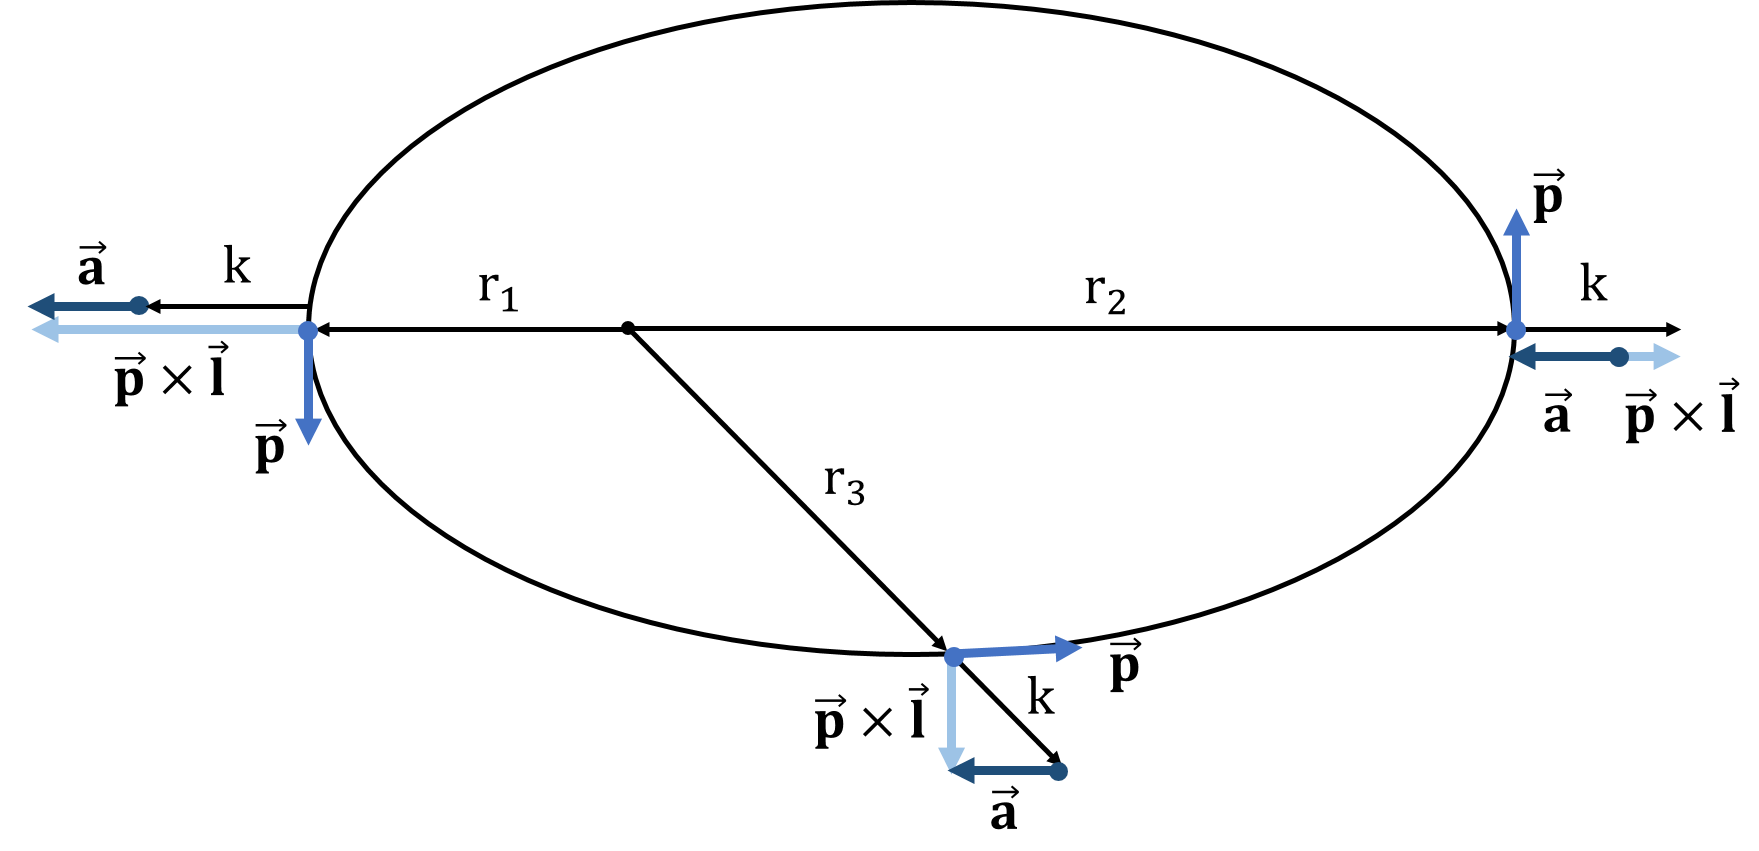
\includegraphics[width=0.9\columnwidth]{clrl.png}
\caption{Kepler orbit with $\vec{r}$,$\vec{l}$ and $\vec{a}$ shown at three different positions. At perihelion $|\vec{p}\times\vec{l}|=k(1+\epsilon)$ and at aphelion $|\vec{p}\times\vec{l}|=k(1-\epsilon)$. The LRL vector $\vec{a}$ always points in the same direction and has the magnitude $|\vec{a}|=k\epsilon$}
\label{fig:clrl}
\end{center}
\end{figure}

We have thus identified two vectorial ($\vec{l}$ and $\vec{a}$) and one scalar ($\mathfrak{e}$) constants of motion, therefore seven conserved quantities in total. In a system with three degrees of freedom and seven constants of motion which are algebraic functions of $\vec{r}$ and $\vec{p}$ that describe the orbit as a whole but not where the particle is located on the orbit at a certain time, we can conclude that not all these are independent. Indeed, because of the two relations connecting this quantities, Properties~\ref{pclrl3} and~\ref{pclrl4}, there are only five independent constants of motion.

\begin{property}\label{pclrl5}
From the properties obtained above, it follows that
\begin{align*}
l^2=mka(1-\epsilon^2),
\end{align*}
where $a$ is the length of the semi-major axis. Thus, the energy of the system can be obtained in a purely algebraic manner
\begin{align*}
\mathfrak{e}=-\frac{k}{2a}.
\end{align*}
\end{property}
\begin{proof}
From Equation~\ref{eclrl} the angle $\theta=0$ corresponds to $r=a(1-\epsilon)$, thus
\begin{align*}
mk\epsilon a(1-\epsilon)=l^2-mka(1-\epsilon)\Rightarrow l^2=mka(1-\epsilon^2).
\end{align*}
The energy of the system can be obtained by substituting this relation, along with $\mathfrak{e}=k\epsilon$, into Property~\ref{pclrl4} and solve for $\mathfrak{e}$.
\end{proof}

One may ask why such an additional conserved quantity exists only in the special case of the Kepler problem and if it would be possible to construct a constant of motion, besides $\mathfrak{e}$ and $\vec{l}$, that describes the orbit for any general central force law. Such conserved quantity can actually be constructed but it turn out to be a rather peculiar function and its existence depends on the condition that the orbit is closed. A remarkable property of a nonclosed orbit it that it will at some moment pass through an arbitrary point characterized by, let's assume, $(r,\theta)$ that is positioned between the bound of the turning points of $r$, or in a more intuitive image, a moving particle must never return to any previous location or the orbit. Therefore, the orbit equation involves an $r$ which is an infinite-valued function of $\theta$ (modulo $2\pi$). If $r$ is $T_r$ periodic and $\theta$ with $T_{\theta}$, the condition of close orbit is given by the integer ratio of the periods $T_r/T_{\theta}$ and these periods are said to be degenerate, as is the case for the Kepler problem.  \\ \indent
Therefore, the mere existence of an additional integral of motion besides the usual $\mathfrak{e}$ and $l$ indicated that the motion is degenerate and that the bounded orbits are closed.

\subsection{Quantum mechanical case}
Since the hydrogen atom presents what it's called an "accidental degeneracy" which can't be explained by the conservation of $\textbf{l}$ and any degeneracy, quantum mechanically speaking, suggests that the system possesses a higher degree of symmetry, there should exist, as in the classical case, an additional operator which is conserved. 
By means of this extra conserved quantity, Pauli discovered an algebraic approach of calculating the energy levels of the hydrogen atom\cite{waerden}, which nowadays can be more generally categorised as an $\mathfrak{so}(4)$ Lie algebraic method. \\ \indent
Due to the fact that $(\textbf{p}\times\textbf{l})^{\dag}=-\textbf{l}^{\dag}\times\textbf{p}^{\dag}=-\textbf{l}\times\textbf{p}$ and similarly $(\textbf{l}\times\textbf{p})^{\dag}=-\textbf{p}^{\dag}\times\textbf{l}^{\dag}=-\textbf{p}\times\textbf{l}$, the hermiticity of the quantum mechanical analogue of the LRL vector $\textbf{a}$ has to be assured by the symmetrization
\begin{equation}\label{eqlrl1}
\textbf{a}=\frac{1}{2m}\left(\textbf{p}\times\textbf{l}-\textbf{l}\times\textbf{p}\right)-k\frac{\textbf{r}}{r} \xrightarrow{a.u.} \frac{1}{2}\left(\textbf{p}\times\textbf{l}-\textbf{l}\times\textbf{p}\right)-\mathcal{Z}\frac{\textbf{r}}{r},
\end{equation}
where atomic units are used $\hbar=m=e=1$ and $\mathcal{Z}$ is the atomic number.

\begin{remark}
In the expression of the QLRL vector as written in Equation~\ref{eqlrl1} the operator $\textbf{r}$ is being introduced. In order to comprehend the manner in which such an operator would act on a certain state, a brief mathematical excursion is required \cite{baran}. \\ 
This operator can be expressed as $x=\sum_i x_i^2$, where $x_i$ with $i=\overline{1,3}$ being the operators associated to the Cartesian coordinates, and is a positive definite operator: if $\bra{\Psi}x\ket{\Psi}\geq 0$ for any $\ket{\Psi}$ and $\bra{\Psi}x\ket{\Psi}=0\Rightarrow\ket{\Psi}=0$. The spectrum of $x$ is in this case non-negative. \\ 
For every Hermitian positive-definite operator such as $x$, another operator with the same properties can be defined such that $r^2=x\Rightarrow r=\sqrt{x}$. This operator has the properties

\begin{noindlist}
\item Same eigenvectors as $x$: $x\ket{\Psi}=\psi_x\ket{\Psi}\Rightarrow r\ket{\Psi}=\psi_r\ket{\Psi}$.
\item Commutes with every operator that commutes with $x$: $[x,y]=0\Rightarrow[r,y]=0$ for any $y$.
\item Has $\sqrt{\psi_x}$ as eigenvalues, where $\psi_x$ are the eigenvalues of $x$: $x\ket{\Psi}=\psi_x\ket{\Psi}\Rightarrow r\ket{\Psi}=\sqrt{\psi_x}\ket{\Psi}$.
\end{noindlist}
\indent The inverse operator $r^{-1}$ has the property that $r r^{-1}=r^{-1} r=I$. If the spectrum of $r$ is ${\psi_r}$ then the spectrum of $\frac{1}{r}$ is $\left\lbrace\frac{1}{\psi_r}\right\rbrace$ and the two operators have the same eigenvectors.
\end{remark}

\begin{property}
The QLRL vector as defined in Equation~\ref{eqlrl1} is an hermitian operator.
\end{property}
\begin{proof}
\abovedisplayskip=-\baselineskip
\belowdisplayskip=0pt
\abovedisplayshortskip=-\baselineskip
\belowdisplayshortskip=0pt
\begin{align*}
\textbf{a}^{\dag} &= \frac{1}{2}\left((\textbf{p}\times\textbf{l})^{\dag}-(\textbf{l}\times\textbf{p})^{\dag}\right)-\mathcal{Z}\frac{\textbf{r}^{\dag}}{r^{\dag}} \\
&= \frac{1}{2}\left(-\textbf{l}^{\dag}\times\textbf{p}^{\dag}+\textbf{p}^{\dag}\times\textbf{l}^{\dag}\right)-\mathcal{Z}\frac{\textbf{r}}{r} \\
&= \frac{1}{2}\left(-\textbf{l}\times\textbf{p}+\textbf{p}\times\textbf{l}\right)-\mathcal{Z}\frac{\textbf{r}}{r} = \textbf{a}
\end{align*}
\end{proof}

\begin{altform}\mbox{}
\begin{noindlist}
\item 
An extremely convenient expression for the QLRL vector is \cite{adams}
\begin{equation}\label{eqlrl2}
\textbf{a}=\left(\frac{1}{2}\textbf{r}p^2-\textbf{p}(\textbf{r}\cdot\textbf{p})\right)+\textbf{r}h.
\end{equation}
\item 
From Equation~\ref{el7} the QRLR vector can be expressed as
\begin{equation}\label{eqlrl4}
\textbf{a} = \textbf{p}\times\textbf{l}-i\textbf{p}-\mathcal{Z}\frac{\textbf{r}}{r}.
\end{equation}
\end{noindlist}
\end{altform}
\begin{proof}
Only the derivation of Equation~\ref{eqlrl2} will be provided, since the other one is trivial.
\begin{align*}
\textbf{a} &= \frac{1}{2}\left(2\textbf{p}\times\textbf{l}-2i\textbf{p}\right)-\mathcal{Z}\frac{\textbf{r}}{r} \text{ (Equation~\ref{el7})}\\
&= \textbf{p}\times\textbf{l}-i\textbf{p}-\mathcal{Z}\frac{\textbf{r}}{r} \\
&= (\textbf{r}p^2-\textbf{p}(\textbf{r}\cdot\textbf{p}-i))-i\textbf{p}-\mathcal{Z}\frac{\textbf{r}}{r} \text{ (Equation~\ref{el4})}\\
&= \frac{1}{2}\textbf{r}p^2-\textbf{p}(\textbf{r}\times\textbf{p})+\textbf{r}\left(\frac{1}{2}p^2-\frac{\mathcal{Z}}{r}\right) \\
&= \left(\frac{1}{2}\textbf{r}p^2-\textbf{p}(\textbf{r}\cdot\textbf{p})\right)+\textbf{r}h
\end{align*}
\end{proof}


\begin{property}
As in the classical case, the QLRL vector $\textbf{a}$ is a constant of motion.
\end{property}
\begin{proof}
A time independent operator is a constant of motion if it commutes with the Hamiltonian, since its total derivative with respect to time can be expressed in the Schrödinger picture as
\begin{equation}\label{eqlrl3}
i\frac{d\textbf{a}}{dt}=[\textbf{a},h],
\end{equation}
where $h$ represents the Hamiltonian of the hydrogen atom:
\begin{equation}\label{eh1}
h=\frac{p^2}{2m}-k\frac{1}{r}\xrightarrow{a.u.}\frac{p^2}{2}-\mathcal{Z}\frac{1}{r}.
\end{equation}

\begin{commutator}
$[\textbf{a},h]=0$
\end{commutator}
\begin{derivation}
In order to show this commutation relation, we use the alternative form of the QRLR vector from Equation~\ref{eqlrl2}
\begin{align*}
[\textbf{a},h]=\left(\left[\frac{1}{2}\textbf{r}p^2,h\right]-[\textbf{p}(\textbf{r}\cdot\textbf{p}),h]\right)+[\textbf{r}h,h].
\end{align*}
\begin{align*}
\left[\frac{1}{2}\textbf{r}p^2,h\right] &= \frac{1}{4}[\textbf{r}p^2,p^2]-\mathcal{Z}\left[\textbf{r}p^2,\frac{1}{r}\right] \\
&= \frac{1}{4}[\textbf{r},p^2]-\frac{\mathcal{Z}}{2}\textbf{r}\left[p^2,\frac{1}{r}\right] \\
&= \frac{1}{4}(2i\textbf{p})p^2-\frac{\mathcal{Z}}{2}\left(2i\frac{1}{r^3}(\textbf{r}\cdot\textbf{p}-i)-\frac{2}{r^3}\right) \\
&\phantom{=} \text{ (Commutators~\ref{crp3} and~\ref{crp4})} \\
&= \left(\frac{1}{2}i\textbf{p}p^2-\mathcal{Z}\frac{i}{r^3}\textbf{r}(\textbf{r}\cdot\textbf{p})\right)
\end{align*}
\begin{align*}
[\textbf{p}(\textbf{r}\cdot\textbf{p}),h] &= \frac{1}{2}[\textbf{p}(\textbf{r}\cdot\textbf{p}),p^2]-\mathcal{Z}\left[\textbf{p}(\textbf{r}\cdot\textbf{p}),\frac{1}{r}\right]\\
&= \frac{1}{2}\textbf{p}[\textbf{r}\cdot\textbf{p},p^2]-\mathcal{Z}\textbf{p}\left[\textbf{r}\cdot\textbf{p},\frac{1}{r}\right]-\mathcal{Z}\left[\textbf{p}.\frac{1}{r}\right](\textbf{r}\cdot\textbf{p}) \\
&= \frac{1}{2}\textbf{p}(2i p^2)-\mathcal{Z}\textbf{p}\left(\frac{i}{r}\right)-\mathcal{Z}\frac{i}{r^3}\textbf{r}(\textbf{r}\cdot\textbf{p}) \\ 
&\phantom{=} \text{ (Commutators~\ref{crp5},~\ref{crp8} and~\ref{crp2} with }f(r)=r^{-1})
\end{align*}
\begin{align*}
[\textbf{r}h,h] = [\textbf{r},h]h=\frac{1}{2}[\textbf{r},p^2]h 
= i\textbf{p}h \text{ (Commutator~\ref{crp3})}
\end{align*} \indent
By combining these expressions, we finally get
\begin{align*}
[\textbf{a},h] = -i\textbf{p}\left(\frac{1}{2}p^2-\frac{\mathcal{Z}}{r}\right)+i\textbf{p}h=0.
\end{align*}
\end{derivation}
After replacing this commutation relation in Equation~\ref{eqlrl3}, the total time derivative of the QRLR becomes zero, thus providing it the property of being a constant of motion.
\end{proof}

Quite similar to the classical case, the QLRL vector satisfies the relations
\begin{noindlist}
\item $\textbf{a}\cdot\textbf{l}=\textbf{l}\cdot\textbf{a}=0$, \eqnum\label{eqlrl5}
\item $a^2=2h(l^2+1)+\mathcal{Z}^2$. \eqnum\label{eqlrl6}
\end{noindlist}
\begin{proof}
An alternative form of the QLRL vector, as expressed in Equation~\ref{eqlrl4}, will be used.
\begin{noindlist}
\item 
Thus, we obtain
\begin{align*}
\textbf{l}\cdot\textbf{a} &= \textbf{l}\cdot(\textbf{p}\times\textbf{l})-i\textbf{l}\cdot\textbf{p}-\mathcal{Z}\textbf{l}\cdot\frac{\textbf{r}}{r} \\
&= \textbf{l}\cdot(\textbf{p}\times\textbf{l}) \text{ (Equations~\ref{el2},~\ref{el3} and Commutator~\ref{cl3})} \\
&= \textbf{l}\cdot(\textbf{r}p^2-\textbf{p}(\textbf{r}\cdot\textbf{p}-i)) \text{ (Equation~\ref{el4})} \\
&= \left((\textbf{l}\cdot\textbf{r})p^2-(\textbf{l}\cdot\textbf{p})(\textbf{r}\cdot\textbf{p}-i)\right) = 0 \text{ (Equations~\ref{el2} and~\ref{el3})},
\end{align*} 
and similarly
\begin{align*}
\textbf{a}\cdot\textbf{l} &= (\textbf{p}\times\textbf{l})\cdot\textbf{l}-i\textbf{p}\cdot\textbf{l}-\mathcal{Z}\frac{\textbf{r}}{r}\cdot\textbf{l} \\
&= (\textbf{p}\times\textbf{l})\cdot\textbf{l} \text{ (Equations~\ref{el2},~\ref{el3} and Commutator~\ref{cl3})} \\
&= (p^2\textbf{r}-(\textbf{p}\cdot\textbf{r}-i)\textbf{p})\cdot\textbf{l} \text{ (Equation~\ref{el4})} \\
&= \left(p^2\textbf{r}\cdot\textbf{l}-(\textbf{p}\cdot\textbf{r}-i)(\textbf{p}\cdot\textbf{l})\right) = 0 \text{ (Equations~\ref{el2} and~\ref{el3})}.
\end{align*} 
\item We first express $a^2$ as
\begin{align*}
a^2 &= \left(\left(\textbf{p}\times\textbf{l}-i\textbf{p}\right)-\mathcal{Z}\frac{\textbf{r}}{r}\right)\cdot\left(\left(\textbf{p}\times\textbf{l}-i\textbf{p}\right)-\mathcal{Z}\frac{\textbf{r}}{r}\right) \\
&= (\textbf{p}\times\textbf{l}-i\textbf{p})^2-\mathcal{Z}\left((\textbf{p}\times\textbf{l}-i\textbf{p})\cdot\frac{\textbf{r}}{r}+\frac{\textbf{r}}{r}\cdot(\textbf{p}\times\textbf{l}-i\textbf{p})\right)-\mathcal{Z}^2,
\end{align*}
and then independently compute the quantities
\begin{align*}
(\textbf{p}\times\textbf{l}-i\textbf{p})^2 &= (\textbf{p}\times\textbf{l})^2-i((\textbf{p}\times\textbf{l})\cdot\textbf{p}+\textbf{p}\cdot(\textbf{p}\times\textbf{l}))-^2p^2 \\
&= p^2l^2-i(2i p^2)-p^2 \text{ (Equations~\ref{el12},~\ref{el9} and~\ref{el8})} \\
&= p^2l^2,
\end{align*}
\begin{align*}
(\textbf{p}\times\textbf{l}-i\textbf{p})\cdot\frac{\textbf{r}}{r} &= (\textbf{p}\times\textbf{l})\cdot\textbf{r}\frac{1}{r}-i\textbf{p}\cdot\textbf{r}\frac{1}{r} \\
&= (l^2+2i\textbf{p}\cdot\textbf{r})\frac{1}{r}-i\textbf{p}\cdot\textbf{r}\frac{1}{r} \text{ (Equation~\ref{el10})} \\
&= \frac{1}{r}l^2+i\textbf{p}\cdot\textbf{r}= \frac{1}{r}l^2+i(\textbf{r}\cdot\textbf{p}-3i),
\end{align*} 
\begin{align*}
\frac{\textbf{r}}{r}\cdot(\textbf{p}\times\textbf{l}-i\textbf{p}) &= \frac{1}{r}\cdot(\textbf{p}\times\textbf{l})-i\frac{1}{r}\textbf{r}\cdot\textbf{p} \\
&= \frac{1}{r}l^2-i\frac{1}{r}\textbf{r}\cdot\textbf{p} \text{ (Equation~\ref{el11})}.
\end{align*}
Therefore, we can finally derive $a^2$ as being
\begin{align*}
a^2 &= p^2(l^2+1)-2k\frac{1}{r}l^2-ik\left((\textbf{r}\cdot\textbf{p})\frac{1}{r}-\frac{1}{r}(\textbf{r}\cdot\textbf{p})\right)-3^2k\frac{1}{r}+\mathcal{Z}^2\\
&= p^2(l^2+1)-2k\frac{1}{r}l^2-ik\left[\textbf{r}\cdot\textbf{p},\frac{1}{r}\right]-3^2k\frac{1}{r}+\mathcal{Z}^2\\
&= p^2(l^2+1)-2k\frac{1}{r}l^2-ik\left(-i r\left(-\frac{1}{r^2}\right)\right)-3^2k\frac{1}{r}+\mathcal{Z}^2 \\
&\phantom{=} \text{ (Commutator~\ref{crp8} with }f(r)=r^{-1}) \\
&= p^2(l^2+1)-2k\frac{1}{r}l^2-2^2k\frac{1}{r}+\mathcal{Z}^2 \\
&= 2\left(\frac{p^2}{2}-\frac{\mathcal{Z}}{r}\right)(l^2+1)+\mathcal{Z}^2 = 2h(l^2+1)+\mathcal{Z}^2.
\end{align*} 
\end{noindlist}
\end{proof}

Finally, a comparison between the classical and quantum LRL vector is made, where the QLRL is expressed in atomic units. We notice that in both cases, the LRL vector is a constant of time and is perpendicular to the angular momentum.
\begin{equation*}
\def\arraystretch{1.3}
\begin{array}{@{}lllllll@{}}
\toprule
\multicolumn{7}{c@{}}{\text{Classical versus quantum LRL vector}}\\
\cmidrule{2-6}
&\text{Quantity} & a & ma^2 & \dot{a} & a\cdot l& \\
\cmidrule{2-6}
&\text{Classical} & \vec{a}=\vec{p}\times\vec{l}-\mathcal{Z}\frac{\vec{r}}{r} & \vec{a}^2=2El^2+mk^2 & \multirow{2}{*}{0} & \multirow{2}{*}{0}& \\ 
&\text{Quantum} & \textbf{a}=\frac{1}{2}\left(\textbf{p}\times\textbf{l}-\textbf{l}\times\textbf{p}\right)-\mathcal{Z}\frac{\textbf{r}}{r} & \textbf{a}^2=2h(l^2+1)+\mathcal{Z}^2 & & & \\
\bottomrule
\end{array}
\end{equation*}

\section{A hydrogenic realization of $\mathfrak{so}(4)$}
The QLRL $\textbf{a}$ vector will be used to build a hydrogenic realization of $\mathfrak{so}(4)$, firstly obtained by Pauli, which can provide the energy levels of the hydrogen atom and can explain what is considered to be an accidentally occurring degeneracy of these levels. This process of constructing a corresponding $\mathfrak{so}(4)$ algebra starting from the known operators $\textbf{l}$ and $\textbf{a}$ begins by simply evaluating their commutators
\begin{equation*}
\begin{aligned}
&[l_i,l_j]=i\epsilon_{ijk}l_k, &&\text{ (Equation~\ref{el1})} \\
&[l_i,a_j]=i\epsilon_{ijk}a_k, &&\text{ (Commutator~\ref{ca1})} \\
&[a_i,a_j]=\left(-2h\right)i\epsilon_{ijk}l_k, &&\text{ (Commutator~\ref{ca2})}
\end{aligned}
\end{equation*}
which reveals the fact that these operators do not close under commutation and do not provide corresponding structure constants in order to form a $\mathfrak{so}(4)$ Lie algebra. However, the QLRL $\textbf{a}$ can be normalized in order to become an appropriate generator. While constructing the normalized version $\textbf{b}$, two distinct cases naturally occur
\begin{equation}\label{eso4.1}
\textbf{b}=\left\{
\begin{array}{ll}
\sqrt{\frac{1}{-2\mathfrak{e}}}\textbf{a},\text{bound states}\rightarrow \mathfrak{so}(4) \text{ Lie algebra: }\sigma=1,\\
\sqrt{\frac{1}{2\mathfrak{e}}}\textbf{a},\text{scattered states}\rightarrow \mathfrak{so}(3,1) \text{ Lie algebra: }\sigma=-1,
\end{array}
\right.
\end{equation}
where, since the system is in a given definite state, the Hamiltonian $h$ was replaced by $\mathfrak{e}$, which represents the energy of the system. The two emerging Lie algebras differ only by the sign of their structure constant involved in the commutation relation of the components belonging to the normalized QLRL: $[b_i,b_j]=\sigma i\epsilon_{ijk}l_k$. Either way, only the case consisting of bound states will be studied, since it generates the $\mathfrak{so}(4)$ Lie algebra that we were looking for and the other case can be treated in a very similar manner. \\ \indent
The obtained QLRL vector
\begin{align*}
\textbf{b}=\frac{1}{\sqrt{-2\mathfrak{e}}}(\textbf{p}\times\textbf{l}-\textbf{l}\times\textbf{p})-\mathcal{Z}\sqrt{\frac{1}{-2\mathfrak{e}}}\frac{\textbf{r}}{r},
\end{align*}
together with $\textbf{l}$ close under commutation and generate a $\mathfrak{so}(4)$ Lie algebra
\begin{equation*}
\begin{aligned}
&[l_i,l_j]=i\epsilon_{ijk}l_k, &&\text{ (Equation~\ref{el1})} \\
&[l_i,b_j]=i\epsilon_{ijk}b_k, &&\text{ (Commutator~\ref{cb1})} \\
&[b_i,b_j]=i\epsilon_{ijk}l_k. &&\text{ (Commutator~\ref{cb2})}
\end{aligned}
\end{equation*}
Thus, the alternative forms of the QLRL vector expressed in Equations~\ref{eqlrl4} and~\ref{eqlrl2} become
\begin{altform}\mbox{}
\begin{noindlist}
\item \abovedisplayskip=-\baselineskip
\belowdisplayskip=0pt
\abovedisplayshortskip=-\baselineskip
\belowdisplayshortskip=0pt
\begin{align*}
&\textbf{a} = \textbf{p}\times\textbf{l}-i\textbf{p}-\mathcal{Z}\frac{\textbf{r}}{r} \rightarrow \sqrt{-2\mathfrak{e}}\textbf{b} = \textbf{p}\times\textbf{l}-i\textbf{p}-\mathcal{Z}\frac{\textbf{r}}{r} \\
& \Rightarrow \textbf{b}=\frac{1}{\sqrt{-2\mathfrak{e}}}\textbf{p}\times\textbf{l}-\frac{i}{\sqrt{-2\mathfrak{e}}}\textbf{p}-\mathcal{Z}\sqrt{\frac{1}{-2\mathfrak{e}}}\frac{\textbf{r}}{r}.
\end{align*}
\item \abovedisplayskip=-\baselineskip
\belowdisplayskip=0pt
\abovedisplayshortskip=-\baselineskip
\belowdisplayshortskip=0pt
\begin{align*}
&\textbf{a}=\left(\frac{1}{2}\textbf{r}p^2-\textbf{p}(\textbf{r}\cdot\textbf{p})\right)+\textbf{r}h \rightarrow \sqrt{-2\mathfrak{e}}\textbf{b}=\left(\frac{1}{2}\textbf{r}p^2-\textbf{p}(\textbf{r}\cdot\textbf{p})\right)+\textbf{r}\mathfrak{e} \\
&\Rightarrow \textbf{b}=\frac{1}{\sqrt{-2\mathfrak{e}}}\left(\frac{1}{2}\textbf{r}p^2-\textbf{p}(\textbf{r}\cdot\textbf{p})\right)+\sqrt{\frac{-\mathfrak{e}}{2}}\textbf{r}.
\end{align*}
\end{noindlist}
\end{altform} \noindent
Two important identities containing the normalized QLRL vector are
\begin{noindlist}
\item $\textbf{b}\cdot\textbf{l}=\textbf{l}\cdot\textbf{b}=0$, \eqnum\label{eso4.2}
\item $b^2=-(l^2+1)-\frac{\mathcal{Z}^2}{2\mathfrak{e}}$. \eqnum\label{eso4.3}
\end{noindlist}
\begin{proof}
By replacing the normalized expression of the QLRL vector from the first row in Equation~\ref{eso4.1} in the previously obtained relations from Equations~\ref{eqlrl5} and~\ref{eqlrl6}, we obtain
\begin{noindlist}
\item \abovedisplayskip=-\baselineskip
\belowdisplayskip=0pt
\abovedisplayshortskip=-\baselineskip
\belowdisplayshortskip=0pt
\begin{align*}
&\textbf{a}\cdot\textbf{l}=\textbf{l}\cdot\textbf{a}=0\Rightarrow \textbf{b}\cdot\textbf{l}=\textbf{l}\cdot\textbf{b}=0
\end{align*}
\item \abovedisplayskip=-\baselineskip
\belowdisplayskip=0pt
\abovedisplayshortskip=-\baselineskip
\belowdisplayshortskip=0pt
\begin{align*}
&a^2=2h(l^2+1)+\mathcal{Z}^2 \Rightarrow b^2=-(l^2+1)-\frac{\mathcal{Z}^2}{2\mathfrak{e}}
\end{align*}
\end{noindlist}
\end{proof}
Finally, the obtained hydrogenic $\mathfrak{so}(4)$ realization may be more conveniently displayed as
\begin{align*}
l_{ij}\Leftrightarrow \begin{bmatrix}
0 & l_3 & -l_2 & b_1 \\
  & 0   & l_1  & b_2 \\
  &     & 0    & b_3 \\
  &     &      & 0   \\
\end{bmatrix},
\end{align*}
expendable to the lower half with the use of antisymmetry. 
The associated Casimir operators are given by
\begin{casimirs}\begin{noindlist}\mbox{}
\item $C^{\mathfrak{so}(4)}_1=l^2+b^2$,
\item $C^{\mathfrak{so}(4)}_2=\frac{1}{2}(\textbf{l}\cdot\textbf{b}+\textbf{b}\cdot\textbf{l})=0$.
\end{noindlist}
\end{casimirs}
\begin{derivation}\mbox{}
\begin{noindlist}
\item
\abovedisplayskip=-\baselineskip
\belowdisplayskip=0pt
\abovedisplayshortskip=-\baselineskip
\belowdisplayshortskip=0pt
\begin{align*}
C^{\mathfrak{so}(4)}_1&=\frac{1}{2}\sum_{i,j}^{1,4}l_{ij}l_{ij}=\sum_{i<j}^{1,4}l_{ij}l_{ij}\\
&=l_3^2+l_2^2+b_1^2+l_1^2+b_2^2+b_3^2=l^2+b^2
\end{align*}
\item 
\begin{align*}
C^{\mathfrak{so}(4)}_2&=\frac{1}{8}\sum_{i,j,k,m}^{1,4}\epsilon_{ijkm}l_{ij}l_{km}=\frac{1}{2}\sum_{i<j,k<m}\epsilon_{ijkm}l_{ij}l_{km}\\
&=\frac{1}{2}(l_3b_3+l_2b_2+b_1l_1+l_1b_1+b_2l_2+b_3l_3)\\
&=\frac{1}{2}(\textbf{l}\cdot\textbf{b}+\textbf{b}\cdot\textbf{l})=0 \text{ Equation~\ref{eso4.2})}
\end{align*}
\end{noindlist}
\end{derivation}

\subsection{Ladder operators for $\mathfrak{so}(4)$}
From Commutator~\ref{cl1}, it follows that $\mathbf{l}$ is an $\mathfrak{so}(3)$ generator and from Commutator~\ref{cb1}, we deduce that $\mathbf{b}$ is an $\mathfrak{so}(3)$ vector operator. In this way, all the study done in Chapter~\ref{ladderso3} may be particularized for $\mathbf{l}$ and $\mathbf{b}$. Hence, in a similar way, we may introduce raising and lowering operators as
\begin{align*}
l_\pm&=l_1\pm il_2,\\
b_\pm&=b_1\pm ib_2,
\end{align*}
such that Equation~\ref{eso3.11} becomes
\begin{equation}\label{eso4.6}
\begin{aligned}
&[l_+,l_-]=2l_3, && [l_3,l_\pm]=\pm l_\pm,\\
&[b_+,b_-]=2l_3, && [b_3,b_\pm]=\pm l_\pm,\\
&[b_+,l_-]=2b_3, &&[b_+,l_+]=0, \\
&[b_-,l_-]=0, &&[b_-,l_+]=-2b_3, \\
&[l_3,b_\pm]=\pm b_\pm, &&[l_\pm,b_3]=\mp b_\pm. \\
\end{aligned}
\end{equation}
Therefore, following Equations~\ref{eso3.22}, we may write
\begin{align*}
l_3\ket{lm}&=m\ket{lm},\\
l_+\ket{lm}&=\mathcal{L}_m^l\ket{l,m+1},\\
l_-\ket{lm}&=\mathcal{L}_{-m}^l\ket{l,m-1},\\
b_3\ket{lm}&=\mathcal{A}_m^l\mathfrak{a}_l\ket{l-1,m}-m\mathfrak{b}_l\ket{lm}+\\
&\phantom{=}+\mathcal{A}_m^{l+1}\mathfrak{a}_{l+1}\ket{l+1,m},\\
b_+\ket{lm}&=\mathcal{B}_m^{l-1}\mathfrak{a}_l\ket{l-1,m+1}-\mathcal{L}_m^l\mathfrak{b}_l\ket{l,m+1}-\\
&\phantom{=}-\mathcal{C}_m^{l+1}\mathfrak{a}_{l+1}\ket{l+1,m+1},\\
b_-\ket{lm}&=-\mathcal{B}_{-m}^{l-1}\mathfrak{a}_l\ket{l-1,m-1}-\mathcal{L}_{-m}^l\mathfrak{b}_l\ket{l,m-1}-\\
&\phantom{=}-\mathcal{C}_{-m}^{l+1}\mathfrak{a}_{l+1}\ket{l+1,m-1},
\end{align*}
where the above coefficients are defined as
\begin{equation}\label{eso4.7}
\begin{aligned}
\mathcal{A}_m^l&=\sqrt{(l-m)(l+m)},\\
\mathcal{B}_m^l&=\sqrt{(l-m+1)(l-m)},\\
\mathcal{C}_m^l&=\sqrt{(l+m+1)(l+m)},\\
\mathcal{L}_m^l&=\sqrt{(l-m)(l+m+1)}.
\end{aligned}
\end{equation}

\subsubsection{Relation between the coefficients $\mathfrak{a}_l$ and $\mathfrak{b}_l$}
By making use the commutation relation $[b_3,b_+]=l_+$ from Equation~\ref{eso4.6} on the basis vector $\ket{lm}$
\begin{align*}
([b_3,b_+]-l_+)\ket{lm}&=(\mathcal{B}_m^{l-1}\mathcal{A}_{m+1}^{l-1}-\mathcal{A}_m^l\mathcal{B}_m^{j-2})\mathfrak{a}_l\mathfrak{a}_{l-1}\ket{l-2,m+1}+\\
&\phantom{=}+((\mathcal{A}_m^l\mathcal{L}_m^{l-1}-(m+1)\mathcal{B}_m^{l-1})\mathfrak{b}_{l-1}+\\
&\phantom{=}+(m\mathcal{B}_m^{l-1}-\mathcal{L}_m^l\mathcal{A}_{m+1}^l)\mathfrak{b}_l)\mathfrak{a}_l\ket{l-1,m+1}+\\
&\phantom{=}+(\mathcal{L}_m^l\mathfrak{b}_l^2-(\mathcal{C}_m^{l+1}\mathcal{A}_{m+1}^{l+1}+\mathcal{A}_m^{l+1}\mathcal{B}_m^l)\mathfrak{a}_{l+1}^2+\\
&\phantom{=}+(\mathcal{B}_m^{l-1}\mathcal{A}_{m+1}^l+\mathcal{A}_m^l\mathcal{C}_m^l)\mathfrak{a}_l^2-\mathcal{L}_m^l)\ket{l,m+1}+\\
&\phantom{=}+(-\mathcal{L}_m^l\mathcal{A}_{m+1}^{l+1}+m\mathcal{C}_m^{l+1})\mathfrak{b}_l+(\mathcal{A}_m^{l+1}\mathcal{L}_m^{l+1}+\\
&\phantom{=}+(m+1)\mathcal{C}_m^{l+1})\mathfrak{c}_{l+1})\mathfrak{a}_{l+1}\ket{l+1,m+1}+\\
&\phantom{=}+(\mathcal{A}_m^{l+1}\mathcal{C}_m^{j+2}-\mathcal{C}_m^{l+1}\mathcal{A}_{m+1}^{l+2})\mathfrak{a}_{l+1}\mathfrak{a}_{l+2}\ket{l+2,m+1},
\end{align*}
and replacing the explicit expressions of the involved coefficients from Equation~\ref{eso4.7}, we get
\begin{align*}
&\mathcal{B}_{m+1}^l((l-1)\mathfrak{b}_{l-1}-(l+1)\mathfrak{b}_l)\mathfrak{a}_l\ket{l-1,m+1}+\\
&+\mathcal{L}_m^l(\mathfrak{b}_l^2-(2l+3)\mathfrak{a}_{l+1}^2+(2l+1)\mathfrak{a}_l^2-1)\ket{l,m+1}-\\
&-\mathcal{C}_{m+1}^l(l\mathfrak{b}_l-(l+2)\mathfrak{b}_{l+1})\mathfrak{a}_{l+1}\ket{l+1,m+1}=0,
\end{align*}
an identity which holds only if
\begin{equation}
\begin{aligned}\label{eso4.8}
(l\mathfrak{b}_l-(l+2)\mathfrak{b}_{l+1})\mathfrak{a}_{l+1}&=0,\\
\mathfrak{b}_l^2-(2l+3)\mathfrak{a}_{l+1}^2+(2l+1)\mathfrak{a}_l^2-1&=0.
\end{aligned}
\end{equation}

\subsubsection{Connection to the hydrogenic realization via Casimir operators}
The associated Casimir operators may also be expressed in terms of the raising and lowering operators as
\begin{align*}
C^{\mathfrak{so}(4)}_1&=l_+l_-+b_+b_-+b_3^2+l_3(l_3-2),\\
C^{\mathfrak{so}(4)}_2&=\frac{1}{2}(b_+l_-+b_-l_+)+b_3l_3,
\end{align*}
which, applied on the basis kets $\ket{jm}$, after the relation between the coefficients $\mathfrak{a}_l$ and $\mathfrak{b}_l$ from Equation~\ref{eso4.8} is used, leads to
\begin{align*}
C^{\mathfrak{so}(4)}_1\ket{lm}&=((l+1)^2\mathfrak{b}_l^2+(4l^2-1)\mathfrak{a}_l^2+l^2-1)\ket{lm},\\
C^{\mathfrak{so}(4)}_2\ket{lm}&=-l(l+1)\mathfrak{b}_l\ket{lm}.
\end{align*}
Let us recall that, for our particular hydrogenic realization involving a scaled QLRL vector $\textbf{b}$, the $\mathfrak{so}(4)$ Casimir operators take the specific forms
\begin{align*}
C^{\mathfrak{so}(4)}_1&=l^2+b^2,\\
C^{\mathfrak{so}(4)}_2&=0,
\end{align*}
from which we may finally obtain the coefficients $\mathfrak{a}_l$ and $\mathfrak{b}_l$ which appear in the $\mathfrak{so}(4)$ ladder operators
\begin{equation}\label{eso4.9}
\begin{aligned}
\mathfrak{b}_l&=0,\\
\mathfrak{a}_l&=\frac{b^2+1}{4l^2-1}.
\end{aligned}
\end{equation}
Therefore, we have:
\begin{equation}\label{eso4.10}
\begin{aligned}
&l^2\ket{lm}=l(l+1)\ket{lm},\\
&C^{\mathfrak{so}(4)}_1\ket{lm}=(l^2+b^2)\ket{lm},\\
&C^{\mathfrak{so}(4)}_2\ket{lm}=0,\\
&l_3\ket{lm}=m\ket{lm},\\
&l_+\ket{lm}=\mathcal{L}_m^l\ket{l,m+1},\\
&l_-\ket{lm}=\mathcal{L}_{-m}^l\ket{l,m-1},\\
&b_3\ket{lm}=\mathcal{A}_m^l\mathfrak{a}_l\ket{l-1,m}+\mathcal{A}_m^{l+1}\mathfrak{a}_{l+1}\ket{l+1,m},\\
&b_+\ket{lm}=\mathcal{B}_m^{l-1}\mathfrak{a}_l\ket{l-1,m+1}-\mathcal{C}_m^{l+1}\mathfrak{a}_{l+1}\ket{l+1,m+1},\\
&b_-\ket{lm}=-\mathcal{B}_{-m}^{l-1}\mathfrak{a}_l\ket{l-1,m-1}-\mathcal{C}_{-m}^{l+1}\mathfrak{a}_{l+1}\ket{l+1,m-1},
\end{aligned}
\end{equation}
with the coefficients $\mathcal{A}_m^l$,$\mathcal{B}_m^l$,$\mathcal{C}_m^l$,$\mathcal{L}_m^l$ given in Equation~\ref{eso4.7} and $\mathfrak{a}_l^m$ from Equation~\ref{eso4.9}.

\subsection{$\mathfrak{so}(4)$ as a $\mathfrak{so}(3)\sim \mathfrak{su}(2)$ coupling problem}
The obtained $\mathfrak{so}(4)$ representation can be viewed as an addition of two angular momenta, by defining the two vector operators
\begin{equation}\label{eso4.4}
\begin{aligned}
\textbf{b}^{+}&=\frac{1}{2}(\textbf{l}+\textbf{b}), \\
\textbf{b}^{-}&=\frac{1}{2}(\textbf{l}-\textbf{b}),
\end{aligned}
\end{equation}
whose components satisfy the commutation relations 
\begin{equation*}
\begin{aligned}
&[b_i^{\pm},b_j^{\pm}]=i\epsilon_{ijk}b_k^{\pm}, &&\text{ (Commutator~\ref{cb+-1})}\\
&[b_i^{+},b_j^{-}]=0. &&\text{ (Commutator~\ref{cb+-2})}
\end{aligned}
\end{equation*}
Thus, $\textbf{b}^{\pm}$ turn out to satisfy the commutation relations characteristic to a $\mathfrak{so}(3)$ Lie algebra and, in this way, actually represent angular momentum vectors. Therefore, $\mathfrak{so}(4)$ may be written as a direct sum $\mathfrak{so}(3)\oplus \mathfrak{so}(3)$ or sub-algebras generated by $\textbf{b}^{\pm}$. 
\begin{remark}
Let $\ket{j_\pm m_\pm}$ denote the vector basis of the two $\mathfrak{so}(3)$ algebras generated by $\textbf{b}^\pm$, from which it follows that their direct product
\begin{align*}
\ket{j_\pm m_\pm}\equiv\ket{j_-m_-}\otimes\ket{j_+m_+},
\end{align*}
determines a representation space for $\mathfrak{so}(4)$. The rigorous manner to write the generators of the two sub-algebras would be
\begin{align*}
\textbf{b}^-\rightarrow \textbf{b}^- \otimes \mathfrak{i}^+, \\
\textbf{b}^+\rightarrow \mathfrak{i}^-\otimes\textbf{b}^+,
\end{align*}
where $\mathfrak{i}^\pm$ represents the identity operator from the $\mathfrak{so}(3)^\pm$ space. For simplicity and always keeping in mind the space on which each operator acts, this notation will be dropped. Further, the usual characteristic eigenvector equations for the involved angular momentum sub-algebras become
\begin{align*}
(\textbf{b}^\pm)^2\ket{j_\pm m_\pm}&= j_\pm(j_\pm+1)\ket{j_\pm m_\pm}, \\
\textbf{b}^\pm_3\ket{j_\pm m_\pm}&= m_\pm\ket{j_\pm m_\pm}.
\end{align*}
This actually represents the vastly studied problem of addition for two angular momenta \cite{zetilli}\cite{sakurai}, in which a proper basis for the coupled system is constructed as $\ket{j_-j_+jm}\equiv\ket{j_\pm jm}$, where $\textbf{b}^\pm=\textbf{b}^-\otimes\mathfrak{i}^++\mathfrak{i}^-\otimes\textbf{b}^+$ is the corresponding angular momentum for the composite system which spans the total space $\mathfrak{so}(3)^-\oplus \mathfrak{so}(3)^+$, with its component $\textbf{b}^\pm_3=\textbf{b}^-_3\otimes\mathfrak{i}^++\mathfrak{i}^-\otimes\textbf{b}^+_3$, operators which satisfy
\begin{align*}
\textbf{b}^\pm\ket{j_\pm jm}&= j(j+1)\ket{j_\pm jm}, \\
\textbf{b}^\pm_3\ket{j_\pm jm}&= m\ket{j_\pm jm}.
\end{align*}
The two vector basis are related through the Clebsch-Gordan coefficients
\begin{align*}
\ket{j_\pm jm}=\sum\limits_{\substack{m_-,m_+ \\ m_-+m_+=m}}\braket{j_\pm m_\pm|j_\pm jm}\ket{j_\pm m_\pm},
\end{align*}
which are non-zero only if $m=m_-+m_+$ and $|j_--j_+|\leq j\leq j_-+j_+$.
\end{remark}
Since the eigenvalues of $(\textbf{b}^\pm)^2$ are $j_\pm(j_\pm+1)$ and both of them can be expressed as
\begin{align*}
(\textbf{b}^\pm)^2 &= \left(\frac{1}{2}(\textbf{l}\pm\textbf{b})\right)^2 \text{ (Equation~\ref{eso4.4})}\\
&= \frac{1}{4}(l^2\pm\textbf{l}\cdot\textbf{b}\pm\textbf{b}\cdot\textbf{l}+b^2) \\
&= \frac{1}{4}(l^2+b^2) \text{ (Equation~\ref{eso4.2})},
\end{align*}
it follows that $j_-=j_+$, thus this realization of $\mathfrak{so}(4)$ using a normalized QLRL vector provides only the diagonal representations. 
The two Casimir operators of $\mathfrak{so}(4)$ can be obtained as linear combinations of the quadratic Casimir operators $\left(\textbf{b}^{\pm}\right)^2$ belonging to the two $\mathfrak{so}(3)$ subalgebras \cite{wybourne}:
\begin{align*} 
C_{\pm}^{\mathfrak{so}(4)}=\left(\textbf{b}^+\right)^2 \pm \left(\textbf{b}^-\right)^2,
\end{align*}
but due to the particular expressions of $\textbf{b}^{\pm}$, only one of them turn out to be non-zero:
\begin{align*}
C_{\pm}^{\mathfrak{so}(4)}&=\left(\frac{1}{2}(\textbf{l}+\textbf{b})\right)^2 \pm \left(\frac{1}{2}(\textbf{l}-\textbf{b})\right)^2 \text{ (Equation~\ref{eso4.4})} \\
&= \frac{1}{4}\left((l^2+\textbf{l}\cdot\textbf{b}+\textbf{b}\cdot\textbf{l}+b^2)\pm(l^2-\textbf{l}\cdot\textbf{b}-\textbf{b}\cdot\textbf{l}+b^2)\right) \\
&= \frac{1}{4}(l^2+b^2)(1\pm 1)+\frac{1}{4}(\textbf{l}\cdot\textbf{b}+\textbf{b}\cdot\textbf{l})(1\mp 1) \\
&= \frac{1}{4}(l^2+b^2)(1\pm 1) \text{ (Equation~\ref{eso4.2})}, 
\end{align*}
\begin{align*}
\Rightarrow \begin{cases} C_{-}^{\mathfrak{so}(4)}=0, \\ C_{+}^{\mathfrak{so}(4)}=\frac{1}{2}(l^2+b^2).\end{cases}
\end{align*}

\subsubsection{Obtaining the energy levels}
Since $(\textbf{b}^\pm)^2$ can be expressed in terms of $l^2+b^2$, the Casimir operator associated to $\mathfrak{so}(4)$ becomes
\begin{align*}
C^{\mathfrak{so}(4)}_+=\frac{1}{2}(l^2+b^2) = 2(\textbf{b}^\pm)^2 = 2j_\pm(j_\pm+1).
\end{align*}

\begin{figure}[!hbt]
\begin{center}
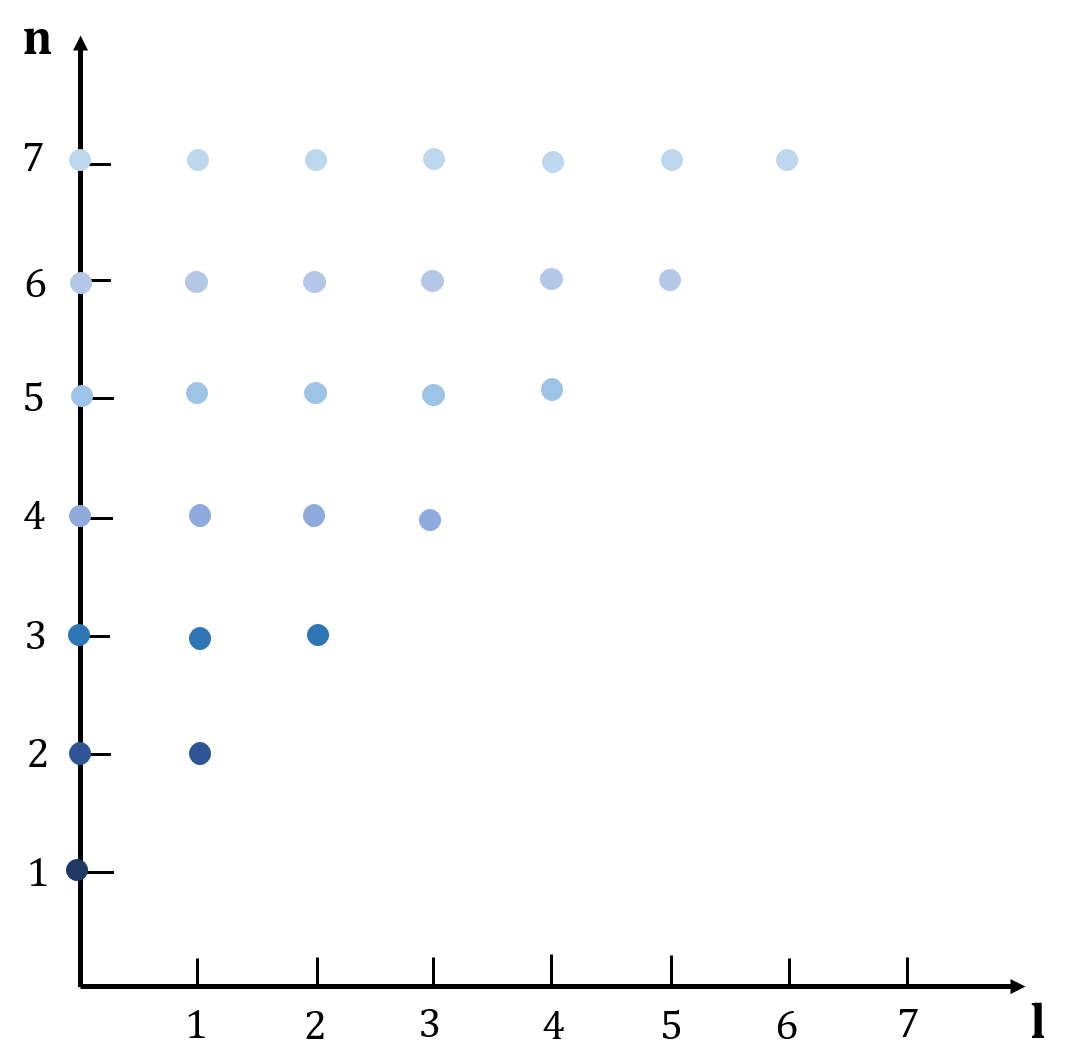
\includegraphics[width=0.7\columnwidth]{tower_1.png}
\caption{A representation of the hydrogenic degeneracies arranged as an infinite tower: each dot represents the $2l+1$-fold orbital degeneracy and the states associated with a given level of the tower have the same energy.}
\label{fig:tower_1}
\end{center}
\end{figure}

By substituting the expression obtained above for $(\textbf{b}^\pm)^2$ in Equation~\ref{eso4.3}
\begin{align*}
(\textbf{b}^\pm)^2 =\frac{1}{4}\left(-1 -\frac{\mathcal{Z}^2}{2\mathfrak{e}}\right),
\end{align*}
and replacing $(\textbf{b}^\pm)^2$ with its corresponding eigenvalue $j_\pm(j_\pm+1)$, the energy of the system can be derived
\begin{align*}
\mathfrak{e}=-\frac{\mathcal{Z}^2}{2(2j_\pm+1)^2},
\end{align*}
where $j$ can have half-integer values. After introducing the notation $n\equiv 2j_\pm+1$, where $n$ would represent the principal quantum number and could take integer values, and then solving for $\mathfrak{e}$, the well-known Bohr formula is obtained
\begin{equation}\label{eso4.5}
\mathfrak{e}_n=-\frac{\mathcal{Z}^2}{2n^2}.
\end{equation}

\subsubsection{Explaining the additional degeneracy}
Now, the so called "accidental degeneracy" of the energy levels can be explained. Since $l^2$ and $l_z$ commute with $h$, we expect that the energies don't depend on $m$. In the framework of the $\mathfrak{so}(3)$ basis alone, from the complete $n^2$-fold degeneracy, only $2l+1$ levels could be accounted for, which are the number of possible energetic levels for a hydrogenic state labeled by $\ket{nlm}$ with fixed $n$ and $l$. From analysis of the $\mathfrak{so}(4)\sim \mathfrak{so}(3)\oplus \mathfrak{so}(3)$ coupled problem, it follows that $j_-=j_+$ and therefore, the degeneracy of an energy level is $\sum_{j_\pm=1}^{n-1}(2j_\pm+1)^2=n^2$, with an additional factor of $2$ required to accommodate the $2$-fold spin degeneracy. Thus, the orbital or degeneracy group of the hydrogen atom is $\mathfrak{so}(4)\sim \mathfrak{so}(3)\oplus \mathfrak{so}(3)$.


\section{A scaled hydrogenic realization of $\mathfrak{so}(4)$}
The scaled $\mathfrak{so}(4)$ realization may be obtained by performing the scaling transformation detailed in Appendix~\ref{scaling}
\begin{align*}
\textbf{r}&=\gamma \textbf{R},\\
\textbf{p}&=\frac{1}{\gamma}\textbf{P},
\end{align*}
were the scaling parameter is chosen as
\begin{align*}
\gamma=\frac{1}{\sqrt{-2\mathfrak{e}}}.
\end{align*}
\begin{remark}
If scattered states are of interest, the $\mathfrak{so}(4,1)$ algebra may be obtained from a scaled $\mathfrak{so}(3,1)$ realization, after applying a scaling transformation with $\gamma=\frac{1}{\sqrt{2\mathfrak{e}}}$.
\end{remark}
By applying this scaling transformation, the QLRL vector becomes:
\begin{equation}\label{eso4scaled.1}
\begin{aligned}
\textbf{B}&=\widetilde{\textbf{b}}=\gamma\left(\frac{1}{2}\widetilde{\textbf{r}}\widetilde{p}^2-\widetilde{\textbf{p}}(\widetilde{\textbf{r}}\cdot \widetilde{\textbf{p}})\right)+\frac{1}{2\gamma}\widetilde{\textbf{r}}\\
&=\gamma\left(\frac{1}{2}\gamma\textbf{R}\frac{1}{\gamma^2}P^2-\frac{1}{\gamma}\textbf{P}\left(\gamma \textbf{R}\cdot \frac{1}{\gamma}\textbf{P}\right)\right)+\frac{1}{2\gamma}\gamma\textbf{R}\\
&= \frac{1}{2}\textbf{R}P^2-\textbf{P}(\textbf{R}\cdot\textbf{P})-\frac{1}{2}\textbf{R},
\end{aligned}
\end{equation}
whereas the angular momentum is invariant under this transformation
\begin{align*}
\textbf{L}=\widetilde{\textbf{l}}=\widetilde{\textbf{r}}\times\widetilde{\textbf{p}}=\gamma\textbf{P}\times\frac{1}{\gamma}\textbf{P}=\textbf{R}\times\textbf{P}.
\end{align*}
Thus, the scaled QLRL and angular momentum close under commutation in order to generate a $\mathfrak{so}(4)$ algebra
\begin{equation}\label{eso41.1}
\begin{aligned}\relax
&[L_i,L_j]=i\epsilon_{ijk}L_k, \\
&[L_i,B_j]=i\epsilon_{ijk}B_k, \\
&[B_i,B_j]=i\epsilon_{ijk}B_k.
\end{aligned}
\end{equation}
Let us notice that the scaled version of Equation~\ref{eso4.2} and~\ref{eso4.3} are
\begin{align*}
&\textbf{B}\cdot\textbf{L}=\textbf{L}\cdot\textbf{B}=0,\\
&B^2+L^2+1=n^2,
\end{align*}
where, in the last formula, the explicit expression for the energy from Equation~\ref{eso4.5}, was used. 
Therefore, the associated ladder operators become
\begin{equation}\label{eso4scaled.2}
\begin{aligned}
&L^2\ket{nlm}=l(l+1)\ket{nlm},\\
&C^{\mathfrak{so}(4)}_1\ket{nlm}=(n^2-1)\ket{nlm},\\
&C^{\mathfrak{so}(4)}_2\ket{nlm}=0,\\
&L_3\ket{nlm}=m\ket{nlm},\\
&L_+\ket{nlm}=\mathcal{L}_m^l\ket{nl,m+1},\\
&L_-\ket{nlm}=\mathcal{L}_{-m}^l\ket{nl,m-1},\\
&B_3\ket{nlm}=\mathcal{A}_m^l\mathfrak{a}_l\ket{l-1,m}+\mathcal{A}_m^{l+1}\mathfrak{a}_{l+1}\ket{n,l+1,m},\\
&B_+\ket{nlm}=\mathcal{B}_m^{l-1}\mathfrak{a}_l\ket{l-1,m+1}-\mathcal{C}_m^{l+1}\mathfrak{a}_{l+1}\ket{n,l+1,m+1},\\
&B_-\ket{nlm}=-\mathcal{B}_{-m}^{l-1}\mathfrak{a}_l\ket{l-1,m-1}-\mathcal{C}_{-m}^{l+1}\mathfrak{a}_{l+1}\ket{n,l+1,m-1},
\end{aligned}
\end{equation}
with the coefficient $\mathfrak{a}_l$ given by
\begin{equation}\label{eso4scaled.3}
\begin{aligned}
\mathfrak{a}_l&=\frac{n^2-l^2}{4l^2-1},
\end{aligned}
\end{equation}
and the coefficients $\mathcal{A}_m^l$,$\mathcal{B}_m^l$,$\mathcal{C}_m^l$,$\mathcal{L}_m^l$ expressed in Equation~\ref{eso4.7}.

\subsubsection{Summary}
\begin{equation*}
\def\arraystretch{1.3}
\begin{array}{@{}ll@{}}
\toprule
 \multicolumn{2}{c@{}}{\text{A scaled hydrogenic }\mathfrak{so}(4) \text{ realization}} \\
\cmidrule{1-2}
 \text{Generators} & \begin{aligned}[t]
 \textbf{L}&=\textbf{R}\times\textbf{P}\\
  \textbf{B}&-\frac{1}{2}\textbf{R}P^2-\textbf{P}(\textbf{R}\cdot\textbf{P})-\frac{1}{2}\textbf{R}\\
  \end{aligned}\\
 \text{Casimir operator} & C^{\mathfrak{so}(4)}=L^2+B^2=n^2-1\\
 \text{Ladder operators} & L_\pm,B_\pm\\
\bottomrule
\end{array}
\end{equation*}

\chapter{$\mathcal{SU}(1,1)\sim \mathcal{SO}(2,1)$ as energy spectrum generating groups}
The energy spectrum of a given system can be deduced from the Casimir operators of the corresponding dynamical or non-compact algebra, in a purely algebraic manner. In the case of the hydrogen atom, the $\mathfrak{su}(1,1)$ and $\mathfrak{so}(2,1)$ Lie algebras provide the means of solving the radial Schrödinger equation, without resorting to the series solutions of second order radial differential equations. \\ \indent
Even though our last algebraic excursion involving $\mathfrak{so}(4)$ made possible the determination of energy levels for the non-relativistic hydrogen atom, it is not expendable to a relativistic analogue. However, the energy spectrum generating algebras provide the means of calculating energy eigenvalues even in the relativistic case.\\ \indent
The associated $\mathfrak{su}(1,1)\sim \mathfrak{so}(2,1)$ generators have no inherent physical significance but their arising form may be simply motivated as being that which allows to express the radial hydrogenic equation as an eigenvalue problem in terms of these generators. \\ \indent 
Further, one of these algebras is required in order to construct the whole spectrum generating algebra of the hydrogen atom, in which mappings from one state to another are possible. This bigger algebra will be obtained by merging the degeneracy algebra $\mathfrak{so}(4)$ with some generators of $\mathfrak{so}(2,1)$ and then introducing new operators in order to close the newly derived algebra.
The generators of the $\mathfrak{su}(1,1)\sim \mathfrak{so}(2,1)$ algebras satisfy the defining commutations:
\begin{equation}\label{esu11.0}
\begin{aligned} \relax
[\gamma_1,\gamma_2]&=-i\gamma_3, \\
[\gamma_2,\gamma_3]&=i\gamma_1, \\
[\gamma_3,\gamma_1]&=i\gamma_2. 
\end{aligned}
\end{equation}
In order to obtain the Casimir operator corresponding to $\mathfrak{su}(1,1)\sim\mathfrak{so}(2,1)$, we will define the complex linear transformation
\begin{align*}
\mathfrak{j}_1&=i\gamma_1, \\
\mathfrak{j}_2&=i\gamma_2, \\
\mathfrak{j}_3&=\gamma_3,
\end{align*}
such that $\mathfrak{j}_i$ with $i=1,2,3$ generate an $\mathfrak{so}(3)$ algebra having as Casimir operator $\mathcal{C}_{\mathfrak{so}(3)}\equiv\mathfrak{j}^2=\mathfrak{j}_1^2+\mathfrak{j}_2^2+\mathfrak{j}_3^2$. In this way, can assume that the Casimir operator for $\mathfrak{su}(1,1)\sim\mathfrak{so}(2,1)$ is given by
\begin{casimir} $\mathcal{C}_{\mathfrak{su}(1,1)\sim\mathfrak{so}(2,1)}\equiv\gamma^2=\gamma_3^2-\gamma_2^2-\gamma_1^2$,
\end{casimir} \noindent
which may be easily verified by checking that $[\gamma^2,\gamma_i]=0$ for $i=1,2,3$.

\section{Ladder operators for $\mathfrak{su}(1,1)\sim\mathfrak{so}(2,1)$}

The raising and lowering operators associated to $\mathfrak{su}(1,1)\sim\mathfrak{so}(2,1)$ will be deduced closely following the calculations done in Section~\ref{ladderso3}, by a direct comparison with $\mathfrak{so}(3)$. It can be easily noticed that the defining commutation relations given in Equation~\ref{esu11.0} differ from the well-known $\mathfrak{so}(3)$ ones only in the minus sign from the first relation. There exist a complex linear transformation that maps the generators of $\mathfrak{su}(1,1)\sim\mathfrak{so}(2,1)$ into those of $\mathfrak{so}(3)$, making them isomorphic complex Lie algebras. \\ \indent
Analogously to the manner in which ladder operators are being introduced in the framework of the angular momentum, we define
\begin{align*}
\gamma_+&=\gamma_1+i\gamma_2,\\
\gamma_-&=\gamma_1-i\gamma_2,
\end{align*}
which satisfy the commutation relations
\begin{equation}\label{eladder1}
\begin{aligned} \relax
&[\gamma_+,\gamma_-]=-2\gamma_3,\\
&[\gamma_3,\gamma_\pm]=\pm\gamma_\pm.
\end{aligned}
\end{equation}
Hence, the Casimir operator associated to the $\mathfrak{su}(1,1)\sim\mathfrak{so}(2,1)$ algebra may be written as
\begin{equation}\label{casimirssu1.1so2.1}
\gamma^2=\gamma_3^2-\gamma_3-\gamma_+\gamma_-=\gamma_3^2+\gamma_3-\gamma_-\gamma_+,
\end{equation}
which may be easily verified by calculating
\begin{equation}\label{eladder2}
[\gamma^2,\gamma_i]=0 \text{ (with }i=1,2,3).
\end{equation}
\indent A representation may be obtained by choosing $\gamma^2$ along with one of the components $\gamma_i$ as a set of commuting operators and depending on the choice, two main classes of irreps arise: $\left\lbrace\gamma^2,\gamma_1\right\rbrace$ or $\left\lbrace\gamma^2,\gamma_2\right\rbrace$ for continuum or scattered states and $\left\lbrace\gamma^3,\gamma_3\right\rbrace$ for bound states. \\ 
Since bound states are of interest, we choose $\left\lbrace\gamma^3,\gamma_3\right\rbrace$ as the system of compatible observables, which have, expressed in an appropriate basis, simultaneous eigenvectors
\begin{align*}
\gamma^2\ket{a,b}&=a\ket{a,b}, \\
\gamma_3\ket{a,b}&=b\ket{a,b}.
\end{align*}
\subsubsection{The effect of $\gamma_\pm$ on $\ket{a,b}$}
By applying the commutator $[\gamma_3,\gamma_\pm]$ on the eigenvectors $\ket{a,b}$, we obtain
\begin{align*}
[\gamma_3,\gamma_\pm]&=\pm\gamma_\pm\ket{a,b} \text{ (Equation~\ref{eladder1})}\\
&=(\gamma_3\gamma_\pm-\gamma_\pm\gamma_3)\ket{a,b}= \gamma_3(\gamma_\pm\ket{a,b})-\gamma_\pm(\underbrace{\gamma_3\ket{a,b}}_{b\ket{a,b}}).
\end{align*}
Let us notice that if $\gamma_\pm$ is applied to a $\gamma_3$ eigenvector, the resulting vector is still an eigenket of $\gamma_3$ but having the corresponding eigenvalue increased or decreased by one unit
\begin{align*}
\gamma_3(\gamma_\pm\ket{a,b})=(b\pm 1)(\gamma_\pm\ket{a,b}).
\end{align*}
Further, by applying the commutator $[\gamma^2,\gamma_3]$ on the eigenket $\ket{a,b}$, we get
\begin{align*}
[\gamma^2,\gamma_\pm]&=0 \text{ (Equation~\ref{eladder2})}\\
&=(\gamma^2\gamma_\pm-\gamma_\pm\gamma^2)\ket{a,b}= \gamma^2(\gamma_\pm\ket{a,b})-\gamma_\pm(\underbrace{\gamma^2\ket{a,b}}_{a\ket{a,b}}),
\end{align*}
from which we can conclude that $\gamma_\pm$ applied on a $\gamma_2$ eigenvector does not change its corresponding eigenvalue
\begin{align*}
\gamma^2(\gamma_\pm\ket{a,b})=a\gamma_\pm\ket{a,b},
\end{align*}
such that the effect of the $\mathfrak{su}(1,1)\sim\mathfrak{so}(2,1)$ ladder operators may be inferred
\begin{equation}\label{eladder3}
\gamma_\pm\ket{a,b}=c_\pm\ket{a,b\pm 1}.
\end{equation}

\subsection{Unirreps of $\mathfrak{su}(1,1)\sim\mathfrak{so}(2,1)$}
We will restrict our ladder operators to be adjoint one to another, that is:
\begin{align*}
\gamma_\pm^{\dagger}=\gamma_\mp.
\end{align*}
Let us denote $\gamma_\pm\ket{a,b}=\ket{\psi_\pm}$. Since the Casimir operator written in Equation~\ref{casimirssu1.1so2.1} may also be expressed as
\begin{align*}
\gamma^2=\gamma_3+\frac{1}{2}(\gamma_-\gamma_++\gamma_+\gamma_-)\Rightarrow\gamma^2-\gamma_3=\frac{1}{2}(\gamma_-\gamma_++\gamma_+\gamma_-),
\end{align*}
which provides the means to express the following quantity in two different ways
\begin{align*}
\bra{a,b}(\gamma^2-\gamma_3)\ket{a,b}&=\frac{1}{2}\bra{a,b}(\gamma_-\gamma_++\gamma_+\gamma_-)\ket{a,b} \\
\Rightarrow a-b^2&=\underbrace{\frac{1}{2}(\braket{\psi_-|\psi_-}+\braket{\psi_+|\psi_+})}_{\geq 0}.
\end{align*}
We may conclude that $a\geq b^2$, such that all unirreps of $\mathfrak{su}(1,1)\sim\mathfrak{so}(2,1)$ are infinite dimensional. \\ \indent
Since the eigenvalue spectra of the operator $\gamma_3$ was chosen to be bounded below and by applying successively  $\gamma_-$, the eigenvalue $b$ is lowered in steps of units, it is expected that there exists $b_{min}$ such that
\begin{align*}
\gamma_-\ket{a,b_{min}}=0.
\end{align*} 
By applying $\gamma_+$ on the previous relation and expressing $\gamma_+\gamma_-$ from Equation~\ref{casimirssu1.1so2.1}, we obtain
\begin{align*}
\gamma_+\gamma_-\ket{a,b_{min}}=0\Rightarrow \underbrace{(\gamma_3^2+\gamma_3-\gamma^2)}_{b_{min}^2+b_{min}-a}\ket{a,b_{min}}=0,
\end{align*} 
resulting in $a=b_{min}(b_{min}+1)$. In order to obtain the expression for the constants $c_\pm$ from Equation~\ref{eladder3}, we use $\gamma_+\gamma_-$ and $\gamma_-\gamma_+$ from Equation~\ref{casimirssu1.1so2.1} as following
\begin{align*}
\braket{\psi_+|\psi_+}&=\bra{a,b}\gamma_-\gamma_+\ket{a,b}\\
&=\bra{a,b}(\gamma_3^2+\gamma_3-\gamma^2)\ket{a,b} \\
&=-a+b(b+1)=-b_{min}(b_{min}+1)+b(b+1)\\
&=-(b_{min}-b)(b_{min}+b+1),
\end{align*}
and analogously
\begin{align*}
\braket{\psi_-|\psi_-}&=\bra{a,b}\gamma_+\gamma_-\ket{a,b}\\
&=\bra{a,b}(\gamma_3^2-\gamma_3-\gamma^2)\ket{a,b} \\
&=-a+b(b-1)=-b_{min}(b_{min}+1)+b(b-1)\\
&=-(b_{min}+b)(b_{min}-b+1).
\end{align*}
Since $\braket{\psi_\pm|\psi_\pm}\geq 0$, we conclude that $-(b_{min}\mp b)(b_{min}\pm b+1)\geq 0$. Let us notice that $a$ and $b$, hence also $b_{min}$ must be real since they are eigenvalues of the hermitian operators $\gamma^2$ and $\gamma_3$. Finally, we have
\begin{equation}\label{eladder4}
\begin{aligned}
\gamma^2\ket{b,b_{min}}&=b_{min}(b_{min}+1)\ket{b,b_{min}},\\
\gamma_3\ket{b,b_{min}}&=b\ket{b,b_{min}},\\
\gamma_\pm\ket{b,b_{min}}&=\sqrt{-(b_{min}\mp b)(b_{min}\pm b+1)}\ket{b\pm 1,b_{min}}.
\end{aligned}
\end{equation}
Only classes of unirreps whose $\gamma_3$ eigenvalue spectra are bounded below are of interest
\begin{align*}
\mathcal{D}^+(b_{min})=\left\lbrace b=-b_{min}+\beta,\beta=0,1,2,...\right\rbrace \text{ with }b_{min}\leq 0.
\end{align*}
It can be noticed that $b_{min}\rightarrow b_{min}-1$ defines an equivalent unirrep, such that
\begin{equation}\label{eladder5}
\mathcal{D}^+(b_{min}-1)=\left\lbrace b=b_{min}+1+\beta,\beta=0,1,2,...\right\rbrace \text{ with }b_{min}\geq -1.
\end{equation}

\section{A hydrogenic realization of $\mathfrak{su}(1,1)$}
The Lie algebra associated with the non-compact group $\mathcal{SU}(1,1)$ is given by the commutation relations
\begin{equation}\label{esu11.1}
\begin{aligned} \relax
[\alpha_1,\alpha_2]&=-i\alpha_3, \\
[\alpha_2,\alpha_3]&=i\alpha_1, \\
[\alpha_3,\alpha_1]&=i\alpha_2,
\end{aligned}
\end{equation}
where the structure constants were chosen to contain $i$ for physical reasons.

\subsubsection{Solving differential equations}
The aim is to obtain a realization of the $\mathfrak{su}(1,1)$ generators in terms of combinations containing at most second-order differential operators, such that the general form
\begin{equation}\label{esu11.2}
\left(\frac{d^2}{dx^2}+\frac{a}{x^2}+bx^2+c\right)\mathfrak{X}(x)=0,
\end{equation}
where $a,b$ and $c$ are constants but $b$ and $c$ are allowed to depend on the energy $\mathfrak{e}$. This ODE is involved in most of the analytically solvable second-order differential equations containing a single variable, including the radial hydrogenic problem, which may be expressed in terms of these generators, thus obtaining the associated spectrum. \\ \indent
There are many ways of generating an $\mathfrak{su}(1,1)$ realization for this type of general differential equation, by introducing an additional phase operator \cite{martinez} or working on a more general class of potential and then finding the associated generators \cite{lanik}. Following \cite{brajamani}, we will restrict ourselves to a realization of this algebra in terms of second-order derivative operators in a single variable $x$, which may be performed by assuming the general expressions
\begin{align*}
\alpha_i=\mathfrak{a}_i(x)\frac{d^2}{dx^2}+\mathfrak{b}_i(x)\frac{d}{dx}+\mathfrak{c}_i(x),
\end{align*}
where $i=\overline{1,3}$. Further, by setting one of the coefficients $\mathfrak{a}_1=0$, performing a similarity transformation to eliminate another coefficient $\mathfrak{b}_1=0$ and then imposing that the rest of the coefficients close under commutation to generate a proper $\mathfrak{su}(1,1)$ algebra, their explicit expression may be derived. \\ \indent
Without loss of generality, for the simplicity of the calculation involved and to directly obtain a canonical realization, in the sense that the operators are invariant under variable and similarity tranformations, we will assume that the required generators already take the reduced forms \cite{wybourne}
\begin{align*}
\alpha_1&=\frac{d^2}{dx^2}+\mathfrak{a}_1(x), \\
\alpha_2&=i\left(\mathfrak{a}_2(x)\frac{d}{dx}+\mathfrak{a}_3(x)\right),\\
\alpha_3&=\frac{d^2}{dx^2}+\mathfrak{a}_4(x),
\end{align*} 
acting on $\mathcal{C}^\infty([0,\infty))$, which is the space of infinitely differentiable functions $f:[0,\infty)\rightarrow\mathbb{C}$. 
After introducing this relations in the $\mathfrak{su}(1,1)$ commutation relations and then solving the resulting differential equations, the involved coefficients become \cite{treatise}
\begin{align*}
\mathfrak{a}_1&=\frac{\mathfrak{c}_1}{(\mathfrak{c}_2-x)^2}+\frac{(\mathfrak{c}_2-x)^2}{16},\\
\mathfrak{a}_2&=\frac{\mathfrak{c}_2-x}{2},\\
\mathfrak{a}_3&=-\frac{1}{4},\\
\mathfrak{a}_4&=\frac{\mathfrak{c}_1}{(\mathfrak{c}_2-x)^2}-\frac{(\mathfrak{c}_2-x)^2}{16},
\end{align*}
where $\mathfrak{c}_1$ and $\mathfrak{c}_2$ are constants of integration.
\begin{derivation}
By direct calculation, it follows that
\begin{align*}
[\alpha_1,\alpha_2]&=i\left(2\mathfrak{a}_2'\frac{d^2}{dx^2}+(\mathfrak{a}_2''+2\mathfrak{a}_3')\frac{d}{dx}+\mathfrak{a}_3''-\mathfrak{a}_1'\mathfrak{a}_2\right),\\
[\alpha_2,\alpha_3]&=-i\left(2\mathfrak{a}_2'\frac{d^2}{dx^2}+(\mathfrak{a}_2''+2\mathfrak{a}_3')\frac{d}{dx}+\mathfrak{a}_3''-\mathfrak{a}_2\mathfrak{a}_3''\right),\\
[\alpha_3,\alpha_1]&=-2(\mathfrak{a}_1'-\mathfrak{a}_4')\frac{d}{dx}-\mathfrak{a}_1''+\mathfrak{a}_4'',
\end{align*}
which after comparing with Equation~\ref{esu11.2}, gives:
\begin{align*}
2\mathfrak{a}_2'+1&=0,\\
\mathfrak{a}_2''+2\mathfrak{a}_3'&=0,\\
\mathfrak{a}_1'\mathfrak{a}_2-\mathfrak{a}_3''-\mathfrak{a}_4&=0,\\
\mathfrak{a}_2\mathfrak{a}_4'-\mathfrak{a}_3''-\mathfrak{a}_1&=0,\\
2(\mathfrak{a}_4-\mathfrak{a}_1)'-\mathfrak{a}_2&=0,\\
(\mathfrak{a}_4-\mathfrak{a}_1)''-\mathfrak{a}_3&=0.
\end{align*}
We can immediately deduce that
\begin{align*}
\mathfrak{a}_2(x)=\frac{\mathfrak{c}_2-x}{2},
\end{align*}
where $\mathfrak{c}_2$ is a constant. Hence
\begin{align*}
\mathfrak{a}_3=-\frac{1}{4},
\end{align*}
and
\begin{align*}
\mathfrak{a}_1-\mathfrak{a}_4=\mathfrak{a}_2(\mathfrak{a}_4-\mathfrak{a}_1)'=\frac{\mathfrak{a}_2^2}{2}=\frac{(\mathfrak{c}_2-x)^2}{8}.
\end{align*}
Additionally, we have,
\begin{align*}
\mathfrak{a}_1+\mathfrak{a}_4=\mathfrak{a}_2(\mathfrak{a}_1+\mathfrak{a}_4)',
\end{align*}
which after integration yields
\begin{align*}
\mathfrak{a}_1+\mathfrak{a}_4=2\frac{\mathfrak{c}_1}{(\mathfrak{c}_2-x)^2},
\end{align*}
where $\mathfrak{c}_1$ is also a constant of motion. By combining this with the previously obtained relation, we get
\begin{align*}
\mathfrak{a}_1(x)&=\frac{\mathfrak{c}_1}{(\mathfrak{c}_2-x)^2}+\frac{(\mathfrak{c}_2-x)^2}{16},\\
\mathfrak{a}_4&=\frac{\mathfrak{c}_1}{(\mathfrak{c}_2-x)^2}-\frac{(\mathfrak{c}_2-x)^2}{16}.
\end{align*}
\end{derivation}
By setting $\mathfrak{c}_2=0$, we get the generators expressed in terms of a single variable $\mathfrak{c}_1$, which we will simply denote as $\mathfrak{c}$
\begin{align*}
\alpha_1&=\frac{d^2}{dx^2}+\frac{\mathfrak{c}}{x^2}+\frac{x^2}{16}, \\
\alpha_2&=-\frac{i}{2}\left(x\frac{d}{dx}+\frac{1}{2}\right),\\
\alpha_3&=\frac{d^2}{dx^2}+\frac{\mathfrak{c}}{x^2}-\frac{x^2}{16}.
\end{align*} \indent
In order to relate this operators to the hydrogenic radial equation, we will first express the more general class of second-order differential equations characterized by the specific quantities $a,b$ and $c$ given in Equation~\ref{esu11.2}, in terms of the $\mathfrak{su}(1,1)$ generators
\begin{equation}\label{esu11.3}
\left(\left(\frac{1}{2}+8b\right)\alpha_1+\left(\frac{1}{2}-8b\right)\alpha_3+c\right)\mathfrak{X}(x)=0,
\end{equation}
by performing the identification
\begin{equation}\label{esu11.4}
a=-4(C^{\mathfrak{su}(1,1)})^2-\frac{3}{4},
\end{equation}
where $C^{\mathfrak{su}(1,1)}$ is the Casimir operator associated to the $\mathfrak{su}(1,1)$ algebra.
\begin{casimir}\label{su1.1casimir} $C^{\mathfrak{su}(1,1)}=\alpha_3^2-\alpha_2^2-\alpha_1^2=-\frac{\mathfrak{c}}{4}-\frac{3}{16}$.
\end{casimir}

\subsubsection{Connection with the radial hydrogenic equation}
The radial equation arising in the Kepler problem is
\begin{align*}
\left(\frac{d^2}{dr^2}+\frac{2}{r}\frac{d}{dr}+\frac{2\mathcal{Z}}{r}-\frac{l(l+1)}{r^2}+2\mathfrak{e}\right)R(r)=0.
\end{align*}
After making the change of variables $r=x^2$, the involved partial derivatives with respect to $r$ transform as:\
\begin{align*}
\frac{d}{dr}=\frac{dx}{dr}\frac{d}{dx}&=\frac{1}{2x}\frac{d}{dx}, \\
\frac{d^2}{dr^2}=\frac{d}{dr}\left(\frac{1}{2x}\frac{d}{dx}\right)&=\frac{1}{4x^2}\frac{d^2}{dx^2}-\frac{1}{4x^3}\frac{d}{dx}.
\end{align*}
By performing the substitution $R(r)=x^{-3/2}\mathfrak{X}(x)$, the radial hydrogenic equation may be written as
\begin{align*}
\left(\frac{1}{4x^2}\frac{d^2}{dx^2}+\frac{3}{4x^3}\frac{d}{dx}+\frac{2\mathcal{Z}}{x^2}-\frac{l(l+1)}{x^4}+2\mathfrak{e}\right)x^{-\frac{3}{2}}\mathfrak{X}(x)=0,
\end{align*}
which leads to
\begin{align*}
\left(\frac{1}{4x^2}\left(\frac{d^2x^{-\frac{3}{2}}}{dx^2}+2\frac{dx^{-\frac{3}{2}}}{dx}\frac{d}{dx}+x^{-\frac{3}{2}}\frac{d^2}{dx^2}\right)+\frac{3}{4x^3}\left(\frac{dx^{-\frac{3}{2}}}{dx}+x^{-\frac{3}{2}}\frac{d}{dx}\right)+\right.\\
+\left.\frac{2\mathcal{Z}x^{-\frac{3}{2}}}{x^2}-\frac{l(l+1)x^{-\frac{3}{2}}}{x^4}+2\mathfrak{e}x^{-\frac{3}{2}}\right)\mathfrak{X}(x)=0.
\end{align*}
After all the computations are being made and the final result is multiplied with $4x^{7/2}$, we finally obtain
\begin{align*}
\left(\frac{d^2}{dx^2}-\frac{4l(l+1)+\frac{3}{4}}{x^2}+8\mathfrak{e}x^2+8\mathcal{Z}\right)\mathfrak{X}(x)=0,
\end{align*}
such that, after a direct comparison with Equation~\ref{esu11.2}, we get
\begin{align*}
a&= -4l(l+1)-\frac{3}{4},\\
b&= 8\mathfrak{e},\\
c&= 8\mathcal{Z}.
\end{align*}
From Equation~\ref{esu11.4}, the constant $\mathfrak{c}$ involved in the general form of the $\mathfrak{su}(1,1)$ generators is obtained as
\begin{align*}
\mathfrak{c}=-4l(l+1)-\frac{3}{4},
\end{align*}
from which the associated Casimir operator becomes
\begin{align*}
C^{\mathfrak{su}(1,1)}=l(l+1).
\end{align*}
Hence, the final form for the $\mathfrak{su}(1,1)$ generators is
\begin{align*}
\alpha_1&=\frac{d^2}{dx^2}-\frac{4l(l+1)+\frac{3}{4}}{x^2}+\frac{x^2}{16}, \\
\alpha_2&=-\frac{i}{2}\left(x\frac{d}{dx}+\frac{1}{2}\right),\\
\alpha_3&=\frac{d^2}{dx^2}-\frac{4l(l+1)+\frac{3}{4}}{x^2}-\frac{x^2}{16}.
\end{align*}

\subsubsection{Energy levels obtained by means of tilting}
The detailed procedure of obtaining the discrete energy levels is presented in Appendix~\ref{tiltingdiscrete} and mainly consists of applying a tilting transformation depending on a variable chosen such that to diagonalize the $\alpha_3$ generator. The energy levels can simply be derived by solving Equation~\ref{etilt7a} for $\mathfrak{e}$
\begin{align*}
\frac{1+\sqrt{1+4l(l+1)}}{2}+\mathfrak{n}&=\frac{8\mathcal{Z}}{8\sqrt{-2\mathfrak{e}}} \text{ for }\mathfrak{su}(1,1),
\end{align*}
from which the discrete energy spectrum is will be given by
\begin{align*}
\mathfrak{e}=-\frac{\mathcal{Z}^2}{2n^2},
\end{align*}
where the following notation has been introduced
\begin{align*}
n=\mathfrak{n}+l+1 \text{ with }\mathfrak{n}=0,1,2,... \text{ }.
\end{align*}

\subsubsection{Summary}
\begin{equation*}
\def\arraystretch{1.3}
\begin{array}{@{}ll@{}}
\toprule
 \multicolumn{2}{c@{}}{\text{A hydrogenic }\mathfrak{su}(1,1) \text{ realization}} \\
\cmidrule{1-2}
 \text{Generators} & \begin{aligned}[t]
  \alpha_1&=\frac{d^2}{dx^2}-\frac{4l(l+1)+\frac{3}{4}}{x^2}+\frac{x^2}{16} \\
\alpha_2&=-\frac{i}{2}\left(x\frac{d}{dx}+\frac{1}{2}\right)\\
\alpha_3&=\frac{d^2}{dx^2}-\frac{4l(l+1)+\frac{3}{4}}{x^2}-\frac{x^2}{16}
  \end{aligned}\\
 \text{Casimir operator} & C^{\mathfrak{su}(1,1)}=l(l+1)\\
\bottomrule
\end{array}
\end{equation*}

\section{A hydrogenic realization of $\mathfrak{so}(2,1)$}
Even though the algebra $\mathfrak{su}(1,1)$ provides the means of obtaining the energy spectrum of the hydrogen atom, due to the particular form of the generators, they may not be further used in order to be merged with the scaled hydrogenic $\mathfrak{so}(4)$ realization and construct a larger algebra in which mappings between different states would be possible. However, an algebra with such generators exist and will be studied in this section. \\ \indent
Since the aim is to use $\mathfrak{so}(2,1)$ as an energy spectrum energy algebra for the hydrogen atom, we seek for a particular realization which can be used to express the Hamiltonian in terms of the resulting generators, thus we look for realizations written in terms of $r$ and $p^2$ or equivalently, $r$ and $p_r^2$ where $p_r$ is the radial momentum operator. Later, a scaling transformation will be performed such that the set of physical operators $\left\lbrace r,p_r \right\rbrace$ will turn to another set $\left\lbrace R,P_R \right\rbrace$, so our realization will be done in terms of $R$ and $P_R$, where the radial momentum is defined as \cite{messiah}
\begin{equation}\label{eso21.5}
\begin{aligned}
P_R&=-i\frac{1}{R}\frac{\partial}{\partial R}R=-i\left(\frac{\partial}{\partial R}+\frac{1}{R}\right)\\
&= \frac{1}{2}(\textbf{R}\cdot\textbf{P}+\textbf{P}\cdot\textbf{R})=\frac{1}{R}(\textbf{R}\cdot\textbf{P}-i).
\end{aligned}
\end{equation}
From this definition, it follows that
\begin{equation}\label{eso21.1}
[R,P_R]=i.
\end{equation}

\subsubsection{Obtaining the generators}
Following \cite{cizekpaldus}, we consider operators taking the form $RP_R^x$ and try to construct from them a proper realization. Since the radial Schrödinger equation associated to the hydrogen atom contains differential operators up to the second order, $x$ can only take the values $0,1,2$. Hence, we start from the set $\left\lbrace R,RP_R,RP_R^2 \right\rbrace$ and check if these operators close under commutation, using Property~\ref{pcom1} and Equation~\ref{eso21.1}
\begin{align*}
[R,RP_R]&=R[R,P_R]=iR, \\
[R,RP_R^2]&=R[R,P_R^2]=R([R,P_R]P_R+P_R[R,P_R])= 2iRP_R, \\
[RP_R,RP_R^2]&= R[P_R,R]P_R^2+R[R,P_R^2]P_R= iRP_R^2.
\end{align*}
Further, we calculate
\begin{align*}
\left[RP_R,\frac{1}{R}\right]&=R\left[\frac{1}{R}(\textbf{R}\cdot\textbf{P}-i),\frac{1}{R}\right]= R\frac{1}{R}\left[\textbf{R}\cdot\textbf{P},\frac{1}{R}\right] \\
&= i\frac{1}{R} \text{ (Property~\ref{crp8} with }f(R)=R^{-1})
\end{align*}
By combining the previously obtained commutators
\begin{align*}
\begin{rcases} \relax
[RP_R,RP_R^2]&=iRP_R^2\\
\left[RP_R,\frac{1}{R}\right]&=i\frac{1}{R}
\end{rcases}
\Rightarrow \left[RP_R,RP_R^2+\mathfrak{b}\frac{1}{R}\right]=i\left(RP_R^2+\mathfrak{b}\frac{1}{R}\right),
\end{align*}
where $\mathfrak{b}$ is an arbitrarily chosen constant. In a similar way
\begin{align*}
\begin{rcases} \relax
[R,RP_R^2]&=2iRP_R\\
\left[R,\frac{1}{R}\right]&=0
\end{rcases}
\Rightarrow \left[R,RP_R^2+\mathfrak{b}\frac{1}{R}\right]=2iRP_R.
\end{align*}
Therefore, we get
\begin{align*}
[RP_R,R]&=-R,\\
\left[RP_R,RP_R^2+\mathfrak{b}\frac{1}{R}\right]&=i\left(RP_R^2+\mathfrak{b}\frac{1}{R}\right),\\
\left[R,RP_R^2+\mathfrak{b}\frac{1}{R}\right]&=2iRP_R.
\end{align*}
Finally, by adding and subtracting the first and second commutation relations, we obtain
\begin{align*}
\left[RP_R,RP_R^2+R+\mathfrak{b}\frac{1}{R}\right]&=i\left(RP_R^2-R+\mathfrak{b}\frac{1}{R}\right),\\
\left[RP_R,RP_R^2-R+\mathfrak{b}\frac{1}{R}\right]&=i\left(RP_R^2+R+\mathfrak{b}\frac{1}{R}\right),\\
\left[R,RP_R^2+\mathfrak{b}\frac{1}{R}\right]&=2iRP_R,
\end{align*}
which after introducing the notations
\begin{equation}\label{so21.5}
\begin{aligned}
\beta_1&=\frac{1}{2}\left(RP_R^2-R+\mathfrak{b}\frac{1}{R}\right), \\
\beta_2&=RP_R, \\
\beta_3&=\frac{1}{2}\left(RP_R^2+R+\mathfrak{b}\frac{1}{R}\right),
\end{aligned}
\end{equation}
become the commutation relations characteristic to an $\mathfrak{so}(2,1)$ Lie algebra
\begin{align*}
[\beta_1,\beta_2]&=-i\beta_3, \\
[\beta_2,\beta_3]&=i\beta_1, \\
[\beta_3,\beta_1]&=i\beta_2. 
\end{align*}

\subsubsection{Connection to the general algebra via the Casimir operator}
In order to connect this realization with the general one obtained in Equation~\ref{eladder4}, which is independent of the particular realization, we have to make an analogy between the eigenvalues of $\beta^2=\beta_3^2-\beta_2^2-\beta_1^2$ with $b_{min}(b_{min}+1)$ and of $\beta_3$ with $b$, therefore to establish a relation between $\mathfrak{b}$,$b_{min}$ and $b$. This can be done by calculating $\beta^2$
\begin{align*}
\beta^2&=(\beta_3^2-\beta_1^2)-\beta_2^2 \\
&=(\beta_3-\beta_1)(\beta_3+\beta_1)-[\beta_3,\beta_1]-\beta_2^2\\
&=R\left(RP_R^2+\mathfrak{b}\frac{1}{R}\right)-iRP_R+(RP_R)^2\\
&=R^2P_R^2+\mathfrak{b}-iRP_R-R(RP_R+[P_R,R])P_R\\
&=\mathfrak{b} \text{ (Equation~\ref{eso21.1})},
\end{align*}
such that we get
\begin{equation}\label{eso21.3}
\mathfrak{b}=b_{min}(b_{min}+1)\Rightarrow b_{min}=\frac{1}{2}\left(-1\pm\sqrt{1+4\mathfrak{b}}\right).
\end{equation}

\subsubsection{Connection to the hydrogenic radial equation}
The Hamiltonian of the hydrogen atom from Equation~\ref{eh1} may be expressed in terms of the radial momentum as:
\begin{align*}
H=\frac{1}{2}p_r^2+\frac{l^2}{2r^2}-\frac{\mathcal{Z}}{r}.
\end{align*}
An appropriate choice  for the constant defining the $\mathfrak{so}(2,1)$ generators would be $\mathfrak{b}=l^2$, such that they can be written as:
\begin{equation}\label{eso21.4}\begin{aligned}
\beta_1&=\frac{1}{2}\left(rp_r^2-r+\frac{l^2}{r}\right),\\
\beta_2&=rp_r,\\
\beta_3&=\frac{1}{2}\left(rp_r^2+r+\frac{l^2}{r}\right).
\end{aligned}
\end{equation}
Hence, the Schrödinger equation may we written as
\begin{align*}
\left(\frac{1}{2}p_r^2+\frac{l^2}{2r^2}-\frac{\mathcal{Z}}{r}\right)\psi(\textbf{r})=\mathfrak{e}\psi(\textbf{r}).
\end{align*}
The wave function of the hydrogen atom expressed in spherical coordinates is separable
\begin{align*}
\psi(\textbf{r})=\psi(r,\theta,\varphi)=\mathfrak{R}(r)Y_{lm}(\theta,\varphi),
\end{align*}
such that the radial equation can be deduced
\begin{equation}\label{eso21.2}
\left(\frac{1}{2}p_r^2+\frac{l^2}{2r^2}-\frac{\mathcal{Z}}{r}-\mathfrak{e}\right)\mathfrak{R}(\textbf{r})=\mathfrak{R}(\textbf{r}),
\end{equation}
which after being multiplied with $2r$ becomes
\begin{align*}
\left(rp_r^2+\frac{l^2}{r}-2\mathcal{Z}-2\mathfrak{e}r\right)\mathfrak{R}(\textbf{r})=0.
\end{align*}
We can easily notice that
\begin{align*}
\beta_3+\beta_1&=rp_r^2+\frac{l^2}{r},\\
\beta_3-\beta_1&=r,
\end{align*}
such that the radial Schrödinger equation can equivalently be written as
\begin{align*}
((1+2\mathfrak{e})\beta_1+(1-2\mathfrak{e})\beta_3-2\mathcal{Z})\mathfrak{R}(\textbf{r})=0.
\end{align*}

\subsubsection{Energy levels obtained by means of scaling}
From this particular form, both the discrete and continuous energy spectra may be obtained, following Appendix~\ref{tiltingdiscrete} and~\ref{tiltingcontinuous}. Nevertheless, in this specific $\mathfrak{so}(2,1)$ realization, there exists a simpler approach to obtaining the energy, without resorting to the tilting transformation, and that is by performing a scaling transformation as that described in Appendix~\ref{scaling}
\begin{align*}
r&=\gamma R,\\
p_r&=\frac{1}{\gamma}P_R.
\end{align*}
Let us notice that the angular momentum operator is invariant to this scaling transformation
\begin{align*}
\textbf{L}=\textbf{R}\times\textbf{P}=\left(\frac{1}{\gamma}\textbf{r}\right)\times(\gamma\textbf{p})=\textbf{r}\times\textbf{p}=\textbf{l}.
\end{align*}
Starting from Equation~\ref{eso21.2} and multiplying it with $r$, we obtain
\begin{align*}
\left(\frac{1}{2}rp_r^2+\frac{l^2}{2r}-\mathcal{Z}-\mathfrak{e}r\right)\mathfrak{R}(\textbf{r})=0,
\end{align*}
which after applying the scaling transformation described above, becomes
\begin{align*}
\left(\frac{1}{2}\left(RP_R^2+\frac{L^2}{R}-2\gamma^2ER\right)-\gamma\mathcal{Z}\right)\mathfrak{R}(\gamma\textbf{R})=0.
\end{align*}
By choosing $\gamma$ such that $2\gamma^2E=-1$ and denoting $\mathfrak{R}(\gamma\textbf{R})=\widetilde{\mathfrak{R}}(\textbf{R})$, an $\beta_3$ eigenvalue equation is obtained
\begin{align*}
(\beta_3-\gamma\mathcal{Z})\widetilde{\mathfrak{R}}(\textbf{R})=0.
\end{align*}
\begin{remark} The choice $2\gamma^2E=1$ would have lead to positive energies corresponding to scattering states and a $\beta_1$ eigenvalues equation.
\end{remark}
From $b_{min}$ calculated from Equation~\ref{eso21.3} with $\mathfrak{b}=\textbf{l}^2$ further replaced by its eigenvalue $l(l+1)$, it follows that
\begin{align*}
b_{min}=\frac{1}{2}(-1\pm(2l+1))\rightarrow \frac{1}{2}(-1+(2l+1))=l,
\end{align*}
where the positive sign was chosen, since $l\geq 0$ and $b_{min}\geq -1$, such that Equation~\ref{eladder5} defining the spectra of the unirrep becomes
\begin{align*}
\mathcal{D}^+(-l-1)=\left\lbrace b=l+1+\beta,\beta=0,1,2,...\right\rbrace \text{ with }b_{min}\geq -1,
\end{align*}
where $b$ is an eigenvalue of $\beta_3$
\begin{align*}
b&=\gamma\mathcal{Z}.
\end{align*}
Therefore, this particular unirrep may be labelled with the Casimir operator
\begin{casimir}\label{casimirso21} $C^{\mathfrak{so}(2,1)}=L^2$
\end{casimir}
\begin{derivation}
Let us recall that $C^{\mathfrak{so}(2,1)}=\beta^2=\beta_3^2-\beta_2^2-\beta_1^2=\mathfrak{b}$ but since the choice $\mathfrak{b}=l^2$ was made, it simply follows that $C^{\mathfrak{so}(2,1)}=L^2$.
\end{derivation}
Finally, the energy is obtained as
\begin{align*}
E=E_{b}=-\frac{\mathcal{Z}^2}{2b^2}=-\frac{\mathcal{Z}^2}{2(l+1+\beta)^2} \text{ with } \beta=0,1,2,...\text{ .}
\end{align*}

\subsubsection{Ladder operators}
Therefore, the associated raising and lowering operators, generally written in Equation~\ref{eladder4}, now knowing that $b_{min}=l$ and $b=n$, take the particular form
\begin{equation}\label{eso21.3}
\begin{aligned}
\beta^2\ket{nlm}&=l(l+1)\ket{nlm},\\
\beta_3\ket{nlm}&=n\ket{nlm},\\
\beta_+\ket{nlm}&=\mathcal{L}_l^n\ket{n+1,lm},\\
\beta_-\ket{nlm}&=\mathcal{L}_l^{-n}\ket{n-1,lm},
\end{aligned}
\end{equation}
with the coefficient $\mathcal{L}_l^n$ defined in Equation~\ref{eso4.7}, with $m=n$.

\subsubsection{Summary}
\begin{equation*}
\def\arraystretch{1.3}
\begin{array}{@{}ll@{}}
\toprule
 \multicolumn{2}{c@{}}{\text{A hydrogenic }\mathfrak{so}(2,1) \text{ realization}} \\
\cmidrule{1-2}
 \text{Generators} & \begin{aligned}[t]
  \beta_1&=\frac{1}{2}\left(rp_r^2+\frac{l^2}{r}-r\right)=\frac{1}{2}(rp^2-r)\\
  \beta_2&=rp_r=\textbf{r}\cdot\textbf{p}-i\\
  \beta_3&=\frac{1}{2}\left(rp_r^2+\frac{l^2}{r}+r\right)=\frac{1}{2}(rp^2+r)
  \end{aligned}\\
 \text{Casimir operator} & C^{\mathfrak{so}(2,1)}=l^2\\
 \text{Ladder operators} & \beta_\pm\\
\bottomrule
\end{array}
\end{equation*}


\chapter{$\mathcal{SO}(4,1)$ and $\mathcal{SO}(4,2)$ as spectrum generating groups}
A larger algebra associated to the hydrogen atom, which not only provides the energy spectrum but also allows the construction of the so called "hydrogenic tower of states" may be obtained by merging the previously obtained algebras $\mathfrak{so}(2,1)$ with $\mathfrak{so}(4)$ to generate an $\mathfrak{so}(4,1)$ Lie algebra. \\ \indent
This will be achieved by firstly merging $\mathfrak{so}(4)$ with the $\mathfrak{so}(2,1)$ generator $\beta_2$, from which a new vector operator similar to the scaled QLRL vector will naturally emerge, thus providing the means to algebraically obtain the ten generators required to close a scaled hydrigenic realization of $\mathfrak{so}(4,1)$. Further, the remaining $\mathfrak{so}(2,1)$ generators $\beta_1$ and $\beta_3$ will be included and since they won't commute with the generators of $\mathfrak{so}(4,1)$, a new vector operator would have to be introduced in order to obtain the fifteen generators of $\mathfrak{so}(4,2)$. \\ \indent
Finally, by applying the raising and lowering operators $B_+$, $L_-$ from $\mathfrak{so}(4)$ and $\beta_-$ from $\mathfrak{so}(2,1)$, any state symbolically denoted by its defining quantum numbers $\ket{nlm}$ may be obtained from the ground state $\ket{100}$.


\section{A scaled hydrogenic realization of $\mathfrak{so}(4,1)$}
An intermediate step in obtaining the $\mathcal{SO}(4,2)$ conformal group of the hydrogen atom would be to obtain one of its subgroups, more precisely the de Sitter group $\mathcal{SO}(4,1)$. The $\mathfrak{so}(4,1)$ algebra is obtained by merging a scaled realization of $\mathfrak{so}(4)$ with the $\mathfrak{so}(2,1)$ generator $\beta_2$.  \\ \indent
Let us notice from Equation~\ref{eso4scaled.1} that there is no energy dependence in the expression of the scaled QLRL vector which generates the scaled $\mathfrak{so}(4)$ realization and only at this point the merging between $\mathfrak{so}(4)$, which is finite dimensional, and a generator of the non-compact $\mathfrak{so}(2,1)$ may be done.\\
It can be easily checked by direct calculation or by observing that the $\mathfrak{so}(2,1)$ generator acts only on the radial part and the $\mathfrak{so}(3)$ generators $\textbf{L}$ on the angular one, that
\begin{align*}
[\beta_2,\textbf{L}]=0. \text{ (Commutator~\ref{cbeta2.1})}
\end{align*}
However, the set $\left\lbrace \beta_2,\textbf{B},\textbf{L}\right\rbrace$ does not close under commutation, since
\begin{align*}
[\beta_2,\textbf{B}]=i\left(\frac{1}{2}\textbf{R}P^2-\textbf{P}(\textbf{R}\cdot\textbf{P})+\frac{1}{2}\textbf{R}\right). \text{ (Commutator~\ref{cbeta2.2})}
\end{align*}
Thus, a new operator needs to be introduced as
\begin{align*}
\textbf{C}=\frac{1}{2}\textbf{R}P^2-\textbf{P}(\textbf{R}\cdot\textbf{P})+\frac{1}{2}\textbf{R}.
\end{align*}
By evaluating the commutators between $\textbf{C}$ and the set of operators $\left\lbrace \beta_2,\textbf{B},\textbf{L}\right\rbrace$ belonging to the scaled $\mathfrak{so}(4)$ and $\mathfrak{so}(2,1)$ realization, the 10 generators of $\mathfrak{so}(4,1)$ from the set $\left\lbrace \beta_2,\textbf{B},\textbf{L}, \textbf{C}\right\rbrace$ are obtained as
\begin{equation*}
\begin{aligned}
&[L_i,L_j]=i\epsilon_{ijk}L_k, &&\text{ (Equation~\ref{eso41.1})}\\
&[L_i,B_j]=i\epsilon_{ijk}B_k, &&\text{ (Equation~\ref{eso41.1})}\\
&[B_i,B_j]=i\epsilon_{ijk}B_k, &&\text{ (Equation~\ref{eso41.1})}\\
&[L_i,C_j]=i\epsilon_{ijk}C_k, &&\text{ (Commutator~\ref{cc1})}\\
&[C_i,C_j]=-i\epsilon_{ijk}L_k, &&\text{ (Commutator~\ref{cc2})}\\
&[B_i,C_j]=i\delta_{ij}\beta_2, &&\text{ (Commutator~\ref{cc3})}\\
&[\beta_2,L_i]=0, &&\text{ (Commutator~\ref{cbeta2.1})}\\
&[\beta_2,B_i]=iC_i, &&\text{ (Commutator~\ref{cbeta2.2})}\\
&[\beta_2,C_i]=iB_i. &&\text{ (Commutator~\ref{cbeta2.3})}
\end{aligned}
\end{equation*}
Let us observe that $[L_i,C_j]=i\epsilon_{ijk}C_k$ shows that $\textbf{C}$ is an $\mathfrak{so}(3)$ vector operator, which along with $[L_i,L_j]=i\epsilon_{ijk}L_k$ and $[C_i,C_j]=-i\epsilon_{ijk}L_k$ prove that $\textbf{L}$ and $\textbf{C}$ generate an $\mathfrak{so}(3,1)$ algebra. 
These generators can be written in a more convenient form as
\begin{align*}
L_{ij}\Longleftrightarrow \begin{bmatrix}
0 & L_3 & -L_2 & B_1      & C_1 \\
  & 0   & L_1  & B_2      & C_2 \\
  &     & 0    & B_3      & C_3 \\
  &     &      & 0        & \beta_2 \\
  &     &      &          & 0
\end{bmatrix},
\end{align*}
extendible to the lower half based on its antisymmetry.
The obtained $\mathfrak{so}(4,1)$ algebra is labeled by 2 independent Casimir operators.
\begin{casimirs}\mbox{}
\begin{noindlist}
\item $C^{\mathfrak{so}(4,1)}_1=L^2+B^2-C^2-\beta_2^2=-2$,
\item $C^{\mathfrak{so}(4,1)}_2=\textbf{D}^2-(\textbf{L}\cdot\textbf{C})^2-(\textbf{L}\cdot\textbf{B})^2=0\text{ where }\textbf{D}=\beta_2\textbf{L}-\textbf{B}\times\textbf{C}$.
\end{noindlist}
\end{casimirs}
\begin{derivation}
Let $M_{\mathfrak{so}(4,1)}$ be the metric matrix associated to $\mathfrak{so}(4,1)$ and defined as
\begin{align*}
M_{\mathfrak{so}(4,1)}=\begin{bmatrix}
I_4 & 0\\
0 & -I_1
\end{bmatrix}=diag(1,1,1,1,-1),
\end{align*}
and let $m_{ij}$ its elements. Then, the associated Casimir operators are:
\begin{noindlist}
\item $C^{\mathfrak{so}(4,1)}_1=\frac{1}{2}\sum_{a,b=1}^{5}L_{ab}L^{ab} \text{ where }L^{ab}=m_{ac}m_{bd}L_{cd}$ 
\begin{align*}
\Rightarrow C^{\mathfrak{so}(4,1)}_1&=\sum_{a<b}^5L_{ab}(m_{aa}m_{bb}L_ab)=\\
&=L_{12}^2+L_{13}^2+L_{14}^2-L_{15}^2+L_{23}^2+L_{24}^2-L_{25}^2+L_{34}^2-L_{35}^2-L_{45}^2\\
&=L_3^2+L_2^2+B_1^2-C_1^2+L_1^2+B_2^2-C_2^2+B_3^2-C_3^2-\beta_2^2\\
&=L^2+B^2-\beta_2^2-C^2\\
&=(\beta_1^2+\beta_2^2-1)+(\beta_3^2-\beta_2^2-\beta_1^2)-\beta_2^2-(\beta_3^2-\beta_2^2+1)\\
&\phantom{=}\text{ (Casimir operator~\ref{casimirso21}, Equations~\ref{eso3} and~\ref{eso4})}\\
&=-2
\end{align*}
\item $C^{\mathfrak{so}(4,1)}_2=\sum_{i,j=1}^{5}m_{ij}w_iw_j \text{ where }w_i=\frac{1}{8}\sum_{a,b,c,d=1}^5\epsilon_{iabcd}L_{ab}L_{cd}$\\
We begin by computing each weight $w_i$ with $i=\overline{1,5}$, making use of the antisymmetry property $L_{ij}=-L_{ji}$.
\begin{align*}
w_1&=L_{23}L_{45}-L_{24}L_{35}+L_{25}L_{34}=L_1\beta_2-B_2C_3+C_2B_3\\
&=\beta_2L_1+[L_1,\beta_2]-(B_2C_3-C_2B_3) \\
&=\beta_2L_1-(\textbf{B}\times\textbf{C})_1 \text{ (Commutator~\ref{cbeta2.1})}
\end{align*}
\begin{align*}
w_2&=-L_{13}L_{45}+L_{14}L_{35}-L_{15}L_{34}=L_2\beta_2+B_1C_3-C_1B_3\\
&=\beta_2L_2+[L_2,\beta_2]-(B_1C_3-C_1B_3) \\
&=\beta_2L_2-(\textbf{B}\times\textbf{C})_2 \text{ (Commutator~\ref{cbeta2.1})}
\end{align*}
\begin{align*}
w_3&=L_{12}L_{45}-L_{14}L_{25}+L_{15}L_{24}=L_3\beta_2+B_1C_2-C_1B_2\\
&=\beta_2L_3+[L_3,\beta_2]-(B_1C_2-C_1B_2) \\
&=\beta_2L_3-(\textbf{B}\times\textbf{C})_3 \text{ (Commutator~\ref{cbeta2.1})}
\end{align*}
\begin{align*}
w_4&=-L_{12}L_{35}+L_{13}L_{25}-L_{15}L_{23}=-L_3C_3-L_2C_2-L_1C_1 = -\textbf{L}\cdot\textbf{C}
\end{align*}
\begin{align*}
w_5&=L_{12}L_{34}-L_{13}L_{24}+L_{14}L_{23}=L_3B_3+L_2B_2+L_1B_1 =\textbf{L}\cdot\textbf{B}
\end{align*}
Thus, we obtain
\begin{align*}
C^{\mathfrak{so}(4,1)}_2&=m_{11}w_1^2+m_{22}w_2^2+m_{33}w_3^2+m_{44}w_4^2+m_{55}w_5^2\\
&=w_1^2+w_2^2+w_3^2+w_4^2-w_5^2\\
&=(\beta_2\textbf{L}-\textbf{B}\times\textbf{C})^2+(\textbf{L}\cdot\textbf{C})^2-(\textbf{L}\cdot\textbf{B})^2\\
&=D^2+(\textbf{L}\cdot\textbf{C})^2-(\textbf{L}\cdot\textbf{B})^2.
\end{align*}
By applying a scaling transformation on the operators from Equation~\ref{eso4.2}, we get
\begin{equation}\label{eso41.3}
\begin{aligned}
\textbf{L}\cdot\textbf{B}=\widetilde{\textbf{l}\cdot\textbf{b}}=0,
\end{aligned}
\end{equation}
from which it follows that
\begin{equation}\label{eso41.2}
\begin{aligned}
\textbf{D}&=i[\textbf{C},\textbf{L}\cdot\textbf{B}]=0, &&\text{ (Commutator~\ref{cblc1})}\\
\textbf{L}\cdot\textbf{C}&=-\frac{i}{3}[\textbf{D},\textbf{B}]=0. &&\text{ (Commutator~\ref{cd1})}\\
\end{aligned}
\end{equation}
Hence $C^{\mathfrak{so}(4,1)}_2=0$, a result which is valid only in this particular hydrogenic realization.
\end{noindlist}
\end{derivation}

\subsection{Ladder operators for $\mathfrak{so}(4,1)$}
In the same way as raising and lowering operators were defined for $\mathfrak{so}(3)$,$\mathfrak{so}(4)$ and $\mathfrak{su}(1,1)\sim\mathfrak{so}(2,1)$, we introduce the ladder operators
\begin{align*}
C_\pm=C_1\pm iC_2,
\end{align*}
which may be expressed in a more convenient form as
\begin{align*}
C_\pm&=-i[\beta_2,B_1]\pm [\beta_2,B_2]) \text{ (Commutator~\ref{cbeta2.2})}\\
&= -i([\beta_2,B_1\pm iB_2])=-i[\beta_2,B_\pm]\\
&=-i\left[-\frac{i}{2}(\beta_+-\beta_-),B_\pm\right]\\
&=-\frac{1}{2}[\beta_+-\beta_-,B_\pm],
\end{align*}
and similarly,
\begin{align*}
C_3&=-i[\beta_2,B_3]\text{ (Commutator~\ref{cbeta2.2})}\\
&=-i\left[-\frac{i}{2}(\beta_+-\beta_-),B_3\right]
\\
&=-\frac{1}{2}[\beta_+-\beta_-,B_3].
\end{align*}
\subsubsection{The effect of $C_\pm$ and $C_3$}
Using the already obtained action of $\beta_\pm$ from Equation~\ref{eso21.3} and $B_\pm$ from Equation~\ref{eso4scaled.2}, we obtain
\begin{align*}
-2C_\pm\ket{nlm}&=(\beta_+-\beta_-)B_\pm\ket{nlm}-B_\pm(\beta_+-\beta_-)\ket{nlm}\\
&=\pm\mathcal{B}_{\pm m}^{l-1}(\mathcal{L}_l^{-n}\mathfrak{a}_l^{n-1}-\mathcal{L}_{l-1}^{-n}\mathfrak{a}_l^n)\ket{n-1,l-1,m\pm 1}\mp\\
&\phantom{=}\mp \mathcal{C}_{\pm m}^{l+1}(\mathcal{L}_{l}^{-n}\mathfrak{a}_{l+1}^{n-1}-\mathcal{L}_{l+1}^{-n}\mathfrak{a}_{l+1}^{n})\ket{n-1,l+1,m\pm 1}\pm\\
&\phantom{=}\pm \mathcal{B}_{\pm m}^{l-1}(\mathcal{L}_{l-1}^{n}\mathfrak{a}_l^{n}-\mathcal{L}_{l}^{n}\mathfrak{a}_l^{n+1})\ket{n+1,l-1,m\pm 1}\mp\\
&\phantom{=}\mp \mathcal{C}_{\pm m}^{l+1}(\mathcal{L}_{l+1}^{n}\mathfrak{a}_{l+1}^{n}-\mathcal{L}_{l}^{n}\mathfrak{a}_{l+1}^{n+1})\ket{n+1,l+1,m\pm 1}.
\end{align*}
Let us define
\begin{equation}\label{eso41.4}
\begin{aligned}
\mathcal{D}_l^n&=\mathcal{L}_l^{-n}\mathfrak{a}_l^{n-1}-\mathcal{L}_{l-1}^{-n}\mathfrak{a}_l^n=\frac{1}{2}\sqrt{\frac{(n+l-1)(n+l)}{(2l-1)(2l+1)}},\\
\mathcal{E}_l^n&=\mathcal{L}_{l-1}^{n}\mathfrak{a}_l^{n}-\mathcal{L}_{l}^{n}\mathfrak{a}_l^{n+1}=\frac{1}{2}\sqrt{\frac{(n-l)(n-l+1)}{(2l-1)(2l+1)}},
\end{aligned}
\end{equation}
such that the action of $C_\pm$ may be expressed as
\begin{equation}\label{eso41.5}
\begin{aligned}
&C_\pm\ket{nlm}=\pm\mathcal{B}_{\pm m}^{l-1}\mathcal{D}_l^n\ket{n-1,l-1,m\pm 1}\pm \mathcal{B}_{\pm m}^{l-1}\mathcal{E}_l^n\ket{n+1,l-1,m\pm 1}\mp\\
&\mp \mathcal{C}_{\pm m}^{l+1}\mathcal{D}_{l+1}^{n-1}\ket{n-1,l+1,m\pm 1}\mp\mathcal{C}_{\pm m}^{l+1}\mathcal{E}_{l+1}^{n+1}\ket{n+1,l+1,m\pm 1}.
\end{aligned}
\end{equation}
In an analogous way, we evaluate
\begin{align*}
-2C_3\ket{nlm}&=(\beta_+-\beta_-)B_3\ket{nlm}-B_3(\beta_+-\beta_-)\ket{nlm}\\
&=\mathcal{A}_{m}^{l}(\mathcal{L}_l^{-n}\mathfrak{a}_l^{n-1}-\mathcal{L}_{l-1}^{-n}\mathfrak{a}_l^n)\ket{n-1,l-1,m}+\\
&\phantom{=}+ \mathcal{A}_{m}^{l+1}(\mathcal{L}_{l}^{-n}\mathfrak{a}_{l+1}^{n-1}-\mathcal{L}_{l+1}^{-n}\mathfrak{a}_{l+1}^{n})\ket{n-1,l+1,m}+\\
&\phantom{=}+ \mathcal{A}_{m}^{l-1}(\mathcal{L}_{l-1}^{n}\mathfrak{a}_l^{n}-\mathcal{L}_{l}^{n}\mathfrak{a}_l^{n+1})\ket{n+1,l-1,m}+\\
&\phantom{=}+ \mathcal{A}_{\pm m}^{l+1}(\mathcal{L}_{l+1}^{n}\mathfrak{a}_{l+1}^{n}-\mathcal{L}_{l}^{n}\mathfrak{a}_{l+1}^{n+1})\ket{n+1,l+1,m},
\end{align*}

from which we obtain
\begin{align*}
C_3\ket{nlm}&=\mathcal{A}_{m}^{l}\mathcal{D}_l^n\ket{n-1,l-1,m}+ \mathcal{A}_{m}^{l}\mathcal{E}_l^n\ket{n+1,l-1,m}+\\
&\phantom{=}\mathcal{A}_{m}^{l+1}\mathcal{D}_{l+1}^{n-1}\ket{n-1,l+1,m}+\mathcal{A}_{m}^{l+1}\mathcal{E}_{l+1}^{n+1}\ket{n+1,l+1,m},
\end{align*}
where $\mathfrak{a}_l^n$ is given in Equation~\ref{eso4scaled.3} and the coefficients $\mathcal{A}_m^l$,$\mathcal{B}_m^l$,$\mathcal{C}_m^l$,$\mathcal{L}_m^l$ are expressed in Equation~\ref{eso4.7}.

\begin{remark}
The associated $\mathcal{SO}(4,1)$ group covers the bound states of the hydrogen atom and contains generators which may create the complete set of quantum numbers $nlm$, such that is is sometimes referred to as the quantum-number group of the hydrogen atom. Even though the enlargement of $\mathcal{SO}(4,1)$ to $\mathcal{SO}(4,2)$ doesn't introduce any additional quantum number and leaves the representation space unmodified, it is needed to introduce an operator which contributes to the construction of the hydrogenic tower of states. 
\end{remark}

\subsubsection{Summary}
\begin{equation*}
\def\arraystretch{1.3}
\begin{array}{@{}ll@{}}
\toprule
 \multicolumn{2}{c@{}}{\text{A scaled hydrogenic }\mathfrak{so}(4,1) \text{ realization}} \\
\cmidrule{1-2}
 \text{Generators} & \begin{aligned}[t]
  \textbf{L}&=\textbf{R}\times\textbf{P}\\
\textbf{B}&=\frac{1}{2}\textbf{R}P^2-\textbf{P}(\textbf{R}\cdot\textbf{P})-\frac{1}{2}\textbf{R}\\
\textbf{C}&=\frac{1}{2}\textbf{R}P^2-\textbf{P}(\textbf{R}\cdot\textbf{P})+\frac{1}{2}\textbf{R}\\
\beta_2&=RP_R=\textbf{R}\cdot\textbf{P}-i
  \end{aligned}\\
 \text{Casimir operator} & C^{\mathfrak{so}(4,1)}=-2\\
\text{Ladder operators} & L_\pm,B_\pm,C_\pm\\
\bottomrule
\end{array}
\end{equation*}

\section{A scaled hydrogenic realization of $\mathfrak{so}(4,2)$}
The $\mathfrak{so}(4,2)$ algebra is obtained by merging the previously derived ten $\mathfrak{so}(4,1)$ generators $\left\lbrace \textbf{L},\textbf{B},\textbf{C},\beta_2 \right\rbrace$ with the two $\mathfrak{so}(2,1)$ remaining operators $\beta_1$ and $\beta_3$. The aim is to generate a larger algebra that includes $\beta_1$, from which the raising and lowering operators $\beta_\pm=\beta_1\pm i\beta_2$ may be obtained. In this way, all three quantum numbers $n,l$ and $m$ will have associated raising and lowering operators, thus allowing mapping between states characterized by different quantum numbers.
We begin our merging process by evaluating the commutators of $\beta_1$ and $\beta_3$ with the $\mathfrak{so}(4,1)$ generators
\begin{equation*}
\begin{aligned}
&[\beta_i,\textbf{L}]=0, &&\text{ (Commutators~\ref{cbeta1.1},~\ref{cbeta2.1} and~\ref{cbeta3.1})}\\
&[\beta_1,\textbf{B}]=i\textbf{F}, &&\text{ (Commutator~\ref{cbeta1.2})}\\
&[\beta_1,\textbf{C}]=0, &&\text{ (Commutator~\ref{cbeta1.3})}\\
&[\beta_3,\textbf{B}]=0, &&\text{ (Commutator~\ref{cbeta3.2})}\\
&[\beta_3,\textbf{C}]=-i\textbf{F}, &&\text{ (Commutator~\ref{cbeta3.3})}
\end{aligned}
\end{equation*}
where a new operator is introduced as
\begin{align*}
\textbf{F}=R\textbf{P},
\end{align*}
and needs to be included in the set of possible generators for $\mathfrak{so}(4,2)$. Its commutators with the the operators from the set $\left\lbrace \textbf{L},\textbf{B},\textbf{C},\beta_1,\beta_2,\beta_3 \right\rbrace$ are
\begin{equation*}
\begin{aligned}
&[F_i,L_j]=i\epsilon_{ijk}F_k, &&\text{ (Commutator~\ref{cf1})}\\
&[F_i,B_j]=-i\delta_{ij}\beta_1, &&\text{ (Commutator~\ref{cf2})}\\
&[F_i,C_j]=-i\delta_{ij}\beta_3, &&\text{ (Commutator~\ref{cf3})}\\
&[F_i,\beta_1]=-iB_i, &&\text{ (Commutator~\ref{cf4})}\\
&[F_i,\beta_2]=0, &&\text{ (Commutator~\ref{cf5})}\\
&[F_i,\beta_3]=-iC_i, &&\text{ (Commutator~\ref{cf6})}\\
&[F_i,F_j]=-i\epsilon_{ijk}L_k. &&\text{ (Commutator~\ref{cf7})}
\end{aligned}
\end{equation*}
Let us notice that the relation $[F_i,L_j]=i\epsilon_{ijk}F_k$ proves that $\textbf{F}$ in an $\mathfrak{so}(3)$ vector operator. The set of 15 operators $\left\lbrace \textbf{L},\textbf{B},\textbf{C},\textbf{F}, \beta_1,\beta_2,\beta_3 \right\rbrace$ generates a scaled hydrogenic $\mathfrak{so}(4,2)$ algebra, which can be written in a more convenient form as
\begin{align*}
L_{ij}\Longleftrightarrow \begin{bmatrix}
0 & L_3 & -L_2 & B_1      & C_1     & F_1 \\
  & 0   & L_1  & B_2      & C_2     & F_2 \\
  &     & 0    & B_3      & C_3     & F_3 \\
  &     &      & 0        & \beta_2 & \beta_1 \\
  &     &      &          & 0       & \beta_3 \\
  &     &      &          &         & 0
\end{bmatrix},
\end{align*}
extendible to the lower half based on its antisymmetry. The following correspondence may be easily seen

\begin{align*}
\begin{rcases}
\mathfrak{so}(3)&\subset\mathfrak{so}(4)\\
\mathfrak{so}(2,1)&\subset\mathfrak{so}(3,1)
\end{rcases}
\subset\mathfrak{so}(4,1)\subset\mathfrak{so}(4,2).
\end{align*}

\begin{remark}
The dynamical group $\mathcal{SO}(4,2)$ has a rich substructure. Its main subgroups are: $\mathcal{SO}(2)\times\mathcal{SO}(4)$, which is the maximal compact subgroup of $\mathcal{SO}(4,2)$, the de Sitter groups $\mathcal{SO}(4,1)$ and $\mathcal{SO}(3,2)$ which is associated with de Sitter spaces of negative curvature, the group $\mathcal{SO}(3,1)$ which is isomorphic to the Lorentz group, the degeneracy group $\mathcal{SO}(4)$, $\mathcal{SO}(2,1)\times\mathcal{SO}(3)$ which is associated  with the separation of the Schrödinger equation into radial and angular part and  $\mathcal{SO}(2,1)\times\mathcal{SO}(2,1)$.
\end{remark}

The three Casimir operators associated to this realization are:
\begin{casimirs}\mbox{}
\begin{noindlist}
\item $C^{\mathfrak{so}(4,2)}_1=L^2+B^2-C^2-F^2+\beta_3^2-\beta_2^2-\beta_1^2=-3$,
\item $C^{\mathfrak{so}(4,2)}_2=-\beta_1(\textbf{C}\cdot\textbf{L})+\beta_2(\textbf{F}\cdot\textbf{L})+\beta_3(\textbf{B}\cdot\textbf{L})-\textbf{B}\cdot(\textbf{C}\times\textbf{F})=0 $,
\item $C^{\mathfrak{so}(4,2)}_3=0$.
\end{noindlist}
\end{casimirs}
\begin{derivation}
Let $M_{\mathfrak{so}(4,2)}$ be the metric matrix associated to $\mathfrak{so}(4,2)$ and defined as
\begin{align*}
M_{\mathfrak{so}(4,2)}=\begin{bmatrix}
I_4 & 0\\
0 & -I_2
\end{bmatrix}=diag(1,1,1,1,-1,-1),
\end{align*}
and let $m_{ij}$ its elements. Then, the associated Casimir operators are:

\begin{noindlist}
\item $C^{\mathfrak{so}(4,2)}_1=\frac{1}{2}L_{ab}L^{ab}\text{ with summation over all indices and }L^{ab}=m_{ac}m_{bd}L_{cd}$
\begin{align*}
C^{\mathfrak{so}(4,2)}_1&=\frac{1}{2}\sum_{a,b}^{1,6}L_{ab}L^{ab}=\sum_{a<b}^6L_{ab}(m_{aa}m_{bb}L_{ab})\\
&=L_{12}^2+L_{13}^2+L_{14}^2-L_{15}^2-L_{16}^2+L_{23}^2+L_{24}^2-L_{25}^2-\\
&\phantom{=}-L_{26}^2+L_{34}^2-L_{35}^2-L_{36}^2-L_{45}^2-L_{46}^2-L_{56}^2\\
&=L_3^2+L_2^2+B_1^2-C_1^2-F_1^2+L_1^2+B_2^2-C_2^2-F_2^2+\\
&\phantom{=}+B_3^2-C_3^2-F_3^2-\beta_2^2-\beta_1^2+\beta_3^2\\
&=(L^2+B^2-C^2-\beta_2^2)-F^2-\beta_1^2+\beta_3^2\\
&=C^{\mathfrak{so}(4,1)}_1-(\beta_3^2-\beta_1^2+1)-\beta_1^2+\beta_3^2\text{ (Identity~\ref{iso42.1})}\\
&=-3
\end{align*}
\item $C^{\mathfrak{so}(4,2)}_2=\frac{1}{48}\epsilon_{abcdef}L^{ab}L^{cd}L^{ef}\text{ with summation over all indices}$
\begin{align*}
C^{\mathfrak{so}(4,2)}_2&=\frac{1}{48}\sum_{a,b,c,d,e,f}^{1,6}\epsilon_{abcdef}L^{ab}L^{cd}L^{ef}\\
&=\frac{1}{48}\left(8\sum\epsilon_{abcdef}L^{ab}L^{cd}L^{ef}\right)\text{ (with }a<b,c<d \text{ and }e<f)\\
&=\frac{1}{6}\left(6\sum_{i,j,k}^{1,3}\epsilon_{ijk}(-L_{i4}L_{j5}L_{k6}+L_{45}L_{i6}L_{jk}-L_{46}L_{i5}L_{jk}+L_{56}L_{i4}L_{jk})\right)\\
&=-L_{14}(L_{25}L_{36}-L_{35}L_{26})-L_{24}(L_{35}L_{16}-L_{15}L_{36})-\\
&\phantom{=}-L_{34}(L_{15}L_{26}-L_{25}L_{16})+L_{45}(L_{16}L_{23}-L_{26}L_{13}+L_{36}L_{12})-\\
&\phantom{=}-L_{46}(L_{15}L_{23}-L_{25}L_{13}+L_{35}L_{12})+L_{56}(L_{14}L_{23}-L_{24}L_{13}+L_{34}L_{12})\\
&=-B_1(C_2F_3-C_3F_2)-B_2(C_3F_1-C_1F_3)-\\
&\phantom{=}-B_3(C_1F_2-C_2F_1)-\beta_2(F_1L_1+F_2L_2+F_3L_3)-\\
&\phantom{=}-\beta_1(C_1L_1+C_2L_2+C_3L_3)+\beta_3(B_1L_1+B_2L_2+B_3L_3)\\
&=-\textbf{B}\cdot(\textbf{C}\times\textbf{F})+\beta_2(\textbf{F}\cdot\textbf{L})-\beta_1(\textbf{C}\cdot\textbf{L})+\beta_3(\textbf{B}\cdot\textbf{L})
\end{align*}
Let us notice that $\textbf{B}\cdot(\textbf{C}\times\textbf{F})=(\textbf{B}\times\textbf{C})\cdot\textbf{F}$ but since, from Equation~\ref{eso41.2} we have $\textbf{D}=\beta_2\textbf{L}-\textbf{B}\times\textbf{C}=0$, it immediately follows that $\textbf{B}\cdot(\textbf{C}\times\textbf{F})=\beta_2(\textbf{L}\cdot\textbf{F})$. By direct calculation, we may derive the relations
\begin{align*}
\textbf{L}\cdot\textbf{F}&=\textbf{L}\cdot R\textbf{P}=R\textbf{L}\cdot\textbf{P}=0, \text{ (Commutator~\ref{cl3} with }f(R)=R)\\
\textbf{F}\cdot\textbf{L}&=R\textbf{P}\cdot\textbf{L}=0.
\end{align*}
From Equations~\ref{eso41.2} and~\ref{eso41.3} we have $\textbf{B}\cdot\textbf{L}=\textbf{C}\cdot\textbf{L}=0$, hence
\begin{align*}
C^{\mathfrak{so}(4,2)}_2=0.
\end{align*}
\item $C^{\mathfrak{so}(4,2)}_3=0$ \cite{cizekpaldusadamsperturbed}
\end{noindlist}
\end{derivation}

\subsection{Ladder operators for $\mathfrak{so}(4,2)$}
In the already usual manner, we define:\
\begin{align*}
F_\pm=F_1\pm iF_2,
\end{align*}
which may be expressed as:\
\begin{align*}
F_\pm&=i[\beta_3,C_1]-[\beta_3,C_2] \text{ (Commutator~\ref{cbeta3.3})}\\
&=i[\beta_3,C_1+iC_2]=i[\beta_3,C_\pm].
\end{align*}
Similarly, we have:\
\begin{align*}
F_3&=i[\beta_3,C_3].\text{ (Commutator~\ref{cbeta3.3})}\\
\end{align*}

\subsubsection{The effect of $F_\pm$ and $F_3$}
From the above simplified expression of $F_\pm$, its action on the kets $\ket{nlm}$ simply derives from that of $\beta_3$, explicitly written in Equation~\ref{eso21.3}, and of $C_\pm$ expressed in Equation~\ref{eso41.5}
\begin{align*}
F_\pm\ket{nlm}&=i\beta_3C_\pm\ket{nlm}-iC_\pm\beta_3\ket{nlm},
\end{align*}
which after performing all the calculations, becomes
\begin{align*}
F_\pm\ket{nlm}&=\mp i\mathcal{B}_{\pm m}^{l-1}\mathcal{D}_l^n\ket{n-1,l-1,m\pm 1}\pm i\mathcal{B}_{\pm m}^{l-1}\mathcal{E}_l^n\ket{n+1,l-1,m\pm 1}\pm\\
&\phantom{=}\pm i\mathcal{C}_{\pm m}^{l+1}\mathcal{D}_{l+1}^{n-1}\ket{n-1,l+1,m\pm 1}\mp i\mathcal{C}_{\pm m}^{l+1}\mathcal{E}_{l+1}^{n+1}\ket{n+1,l+1,m\pm 1}.
\end{align*}
Analogously
\begin{align*}
F_3\ket{nlm}&=i\beta_3C_3\ket{nlm}-iC_3\beta_3\ket{nlm},
\end{align*}
which finally leads to
\begin{align*}
F_3\ket{nlm}&=-i\mathcal{A}_{m}^{l}\mathcal{D}_l^n\ket{n-1,l-1,m}+i\mathcal{A}_{m}^{l}\mathcal{E}_l^n\ket{n+1,l-1,m}-\\
&\phantom{=}-i\mathcal{A}_{m}^{l+1}\mathcal{D}_{l+1}^{n-1}\ket{n-1,l+1,m}+i\mathcal{A}_{m}^{l+1}\mathcal{E}_{l+1}^{n+1}\ket{n+1,l+1,m},
\end{align*}
where $\mathfrak{a}_l^n$ is given in Equation~\ref{eso4scaled.3}, the coefficients $\mathcal{A}_m^l$,$\mathcal{B}_m^l$,$\mathcal{C}_m^l$,$\mathcal{L}_m^l$ are expressed in Equation~\ref{eso4.7} and $\mathcal{D}_l^n$,$\mathcal{E}_l^n$ in Equation~\ref{eso41.4}.

\subsection{Hydrogenic tower of states}
\begin{figure}[!hbt]
\begin{center}
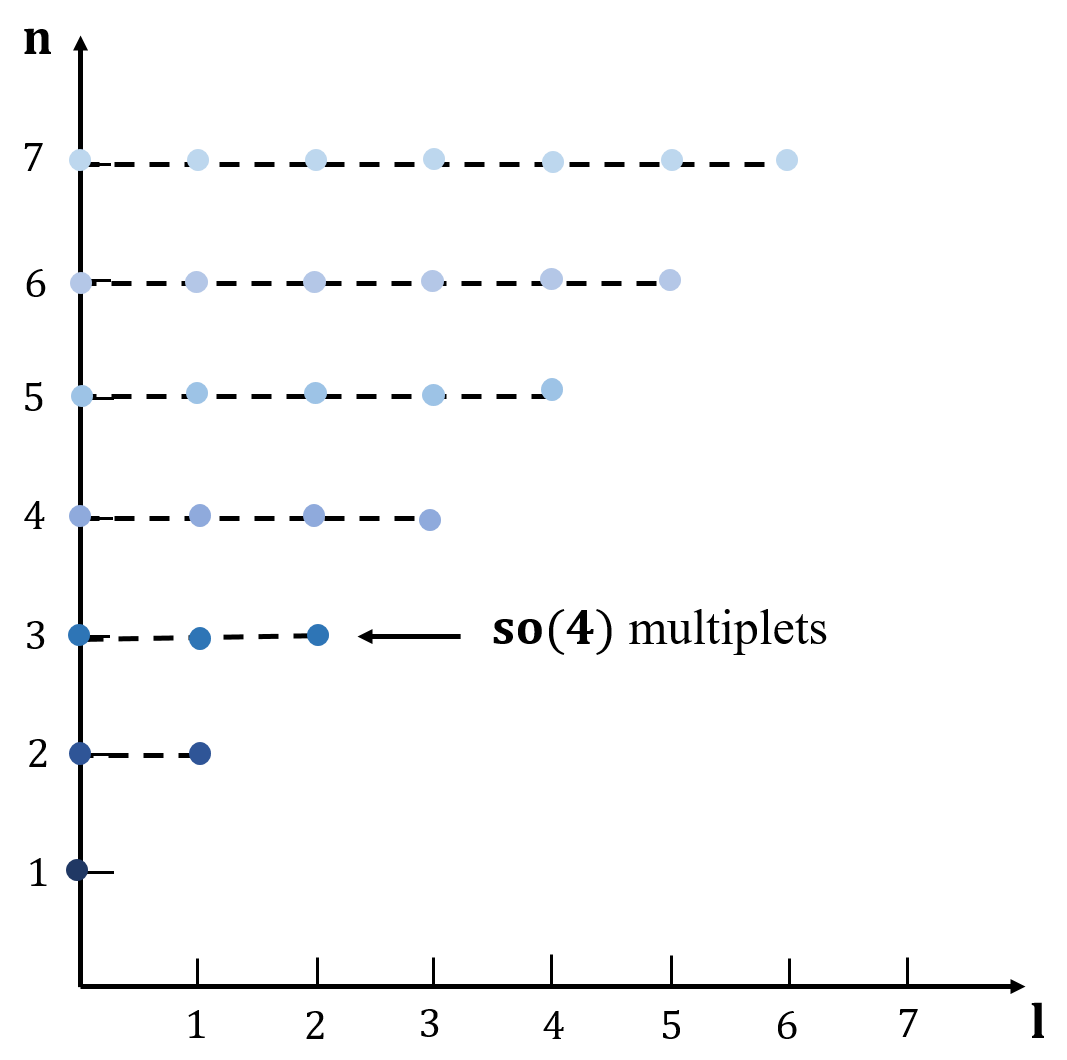
\includegraphics[width=0.7\columnwidth]{tower_3.png}
\caption{The states of the hydrogen atom displayed as an infinite $\mathfrak{so}(4,2)$ tower with $\mathfrak{so}(4)$ multiplets as subtowers\cite{wybourne}}
\label{fig:tower_3}
\end{center}
\end{figure}
The raising and lowering operators of $\mathfrak{so}(4,2)$ $B+,\beta_+$ and $L_-$ may be used to obtain any state given by $\ket{nlm}$ from the ground state $\ket{100}$. Let us create the following configuration: we call a subtower any triangle array of points representing $\ket{nlm}$ states for a fixed value of $n$, where $l=0,1,...,n-1$ and $m=-l,-l+1,...l-1,l$. Any state from such a subtower may be obtained by applying $B_+$, which would allow the movement from the top state $\ket{n00}$, along the right side of the triangle, until the desired $l$ is reached, and then applying $L_-$ to move from right to left, in this way varying $m$.

\begin{figure}[!hbt]
\begin{center}
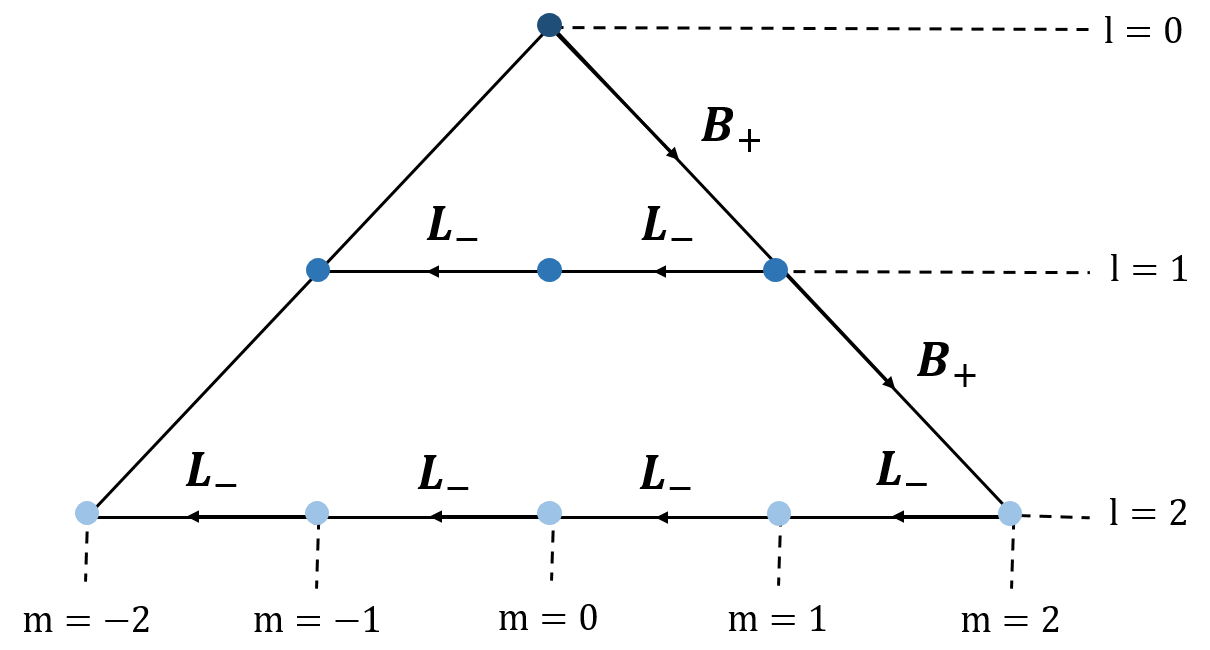
\includegraphics[width=0.9\columnwidth]{tower_2.png}
\caption{An $\mathfrak{so}(4)$ subtower representing scaled hydrogenic states $\ket{3lm}$. Each state may be obtained by successively applying $B_+$ and $L_-$}
\label{fig:tower_2}
\end{center}
\end{figure}

\subsubsection{The effect of $B_+$}
By making the substitution $l=l-1$ and $m=l-1$ in Equation~\ref{eso4scaled.2} for $B_+$, we obtain
\begin{align*}
B_+\ket{n,l-1,l-1}=\underbrace{-\sqrt{\frac{2l(n^2-l^2)}{2l+1}}}_{a^+_{nl}}\ket{nll},
\end{align*}
such that $B_+$ acts as a raising operator which connects states with different $l$ and maximum $m$ values.\\ \indent
By successively applying $B_+$ on the top state, we obtain
\begin{equation}\label{etower1}
\ket{nll}=\frac{1}{\prod_{i=1}^la^+_{ni}}(B_+)^l\ket{n00}.
\end{equation}

\subsubsection{The effect of $L_-$}
Similarly, by replacing $m=m+1$ in Equation~\ref{eso4scaled.2} for $L_-$, we get
\begin{align*}
L_-\ket{nl,m+1}&=\underbrace{\sqrt{(l+m+1)(l-m)}}_{b^-_{lm}}\ket{nlm},
\end{align*}
which, after iterative applications, leads to
\begin{equation}\label{etower2}
\ket{nlm}=\frac{1}{\prod_{i=m}^{l-1}b^-_{li}}(L_-)^{l-m}\ket{nll}.
\end{equation}
By combining Equations~\ref{etower1} and~\ref{etower2}, any state belonging to a subtower defined by a given $n$ may be obtained from the top state as
\begin{equation}\label{etower3}
\ket{nlm}=\frac{1}{\prod_{i=1}^la^+_{ni}\prod_{i=m}^{l-1}b^-_{li}}(L_-)^{l-m}(B_+)^l\ket{n00}.
\end{equation}

\subsubsection{The effect of $\beta_+$}
By replacing $n=n-1$ in Equation~\ref{eso21.3}, we get
\begin{align*}
\beta_+\ket{n-1,lm}=\underbrace{\sqrt{(n-l-1)(n+l)}}_{c^+_{nl},}\ket{nlm}
\end{align*}
which after successive applications leads to
\begin{align*}
\ket{nlm}=\frac{1}{\prod_{i=l+2}^{n}c^+_{il}}(\beta_+)^{n-l-1}\ket{l+1,lm}.
\end{align*}
In order to connect the top of subtowers given by consecutive $n$, we take $l=m=0$ in the previously obtained relation, such that we get
\begin{equation}\label{etower4}
\ket{n00}=\frac{1}{\prod_{i=2}^{n}c^+_{i0}}(\beta_+)^{n-1}\ket{100}.
\end{equation}
Finally, by combining Equations~\ref{etower3} and~\ref{etower4}, we obtain
\begin{align*}
\ket{nlm}=\frac{1}{\prod_{i=1}^la^+_{ni}\prod_{i=m}^{l-1}b^-_{li}\prod_{i=2}^{n}c^+_{i0}}(L_-)^{l-m}(B_+)^l(\beta_+)^{n-1}\ket{100},
\end{align*}
which may be further simplified to
\begin{equation}\label{etower5}
\ket{nlm}=\mathcal{F}_{nlm}(L_-)^{l-m}(B_+)^l(\beta_+)^{n-1}\ket{100},
\end{equation}
where
\begin{align*}
\mathcal{F}_{nlm}=\frac{(-1)^l}{2^ll!(n-1)!}\sqrt{\frac{(2l+1)(n-l-1)!(l+m)!}{(n+l)!(l-m)!}}.
\end{align*}

\begin{figure}[!hbt]
\begin{center}
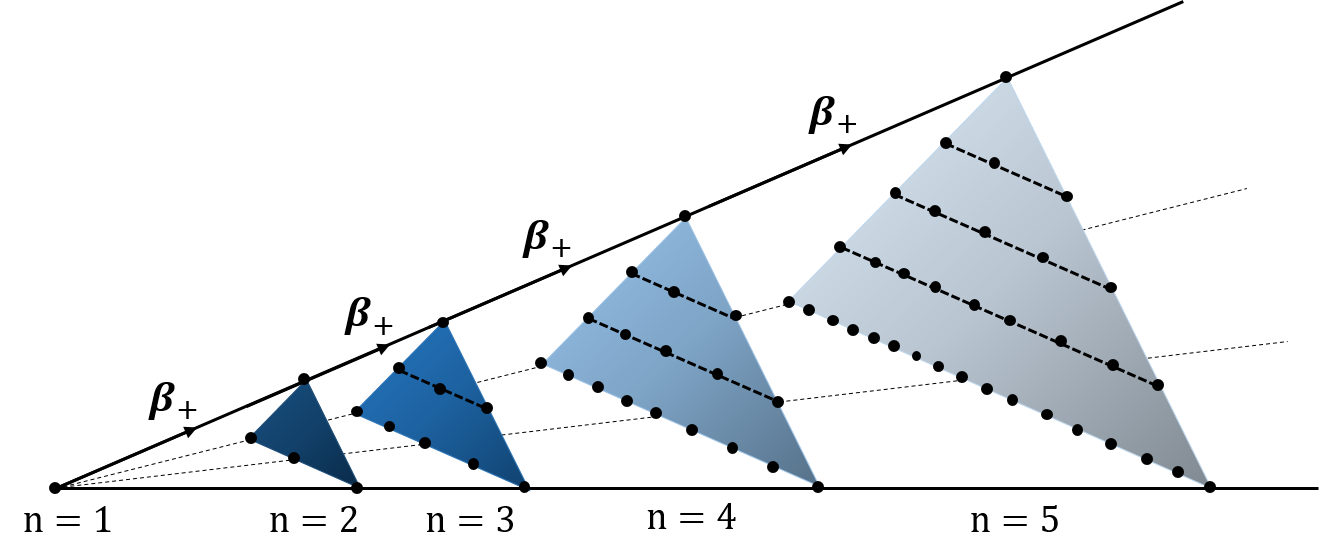
\includegraphics[width=\columnwidth]{tower_4.png}
\caption{Complete $\mathfrak{so}(4,2)$ tower, each $\mathfrak{so}(4)$ subtower being a shaded triangle and the top state in each subtower may be obtained by successive application of $\beta_+$ to the ground state}
\label{fig:tower_4}
\end{center}
\end{figure}

\begin{remark}
Since the generators of $\mathfrak{so}(4,2)$ allow us to move between any hydrogenic states labelled by $\ket{nlm}$ and this hydrogenic realization constitutes an irreducible representation that covers all the states of the hydrogen atom, we may conclude that $\mathcal{SO}(4,2)$ must be a dynamical group for the hydrogen atom.
\end{remark}

\subsubsection{Summary}
\begin{equation*}
\def\arraystretch{1.3}
\begin{array}{@{}ll@{}}
\toprule
 \multicolumn{2}{c@{}}{\text{A scaled hydrogenic }\mathfrak{so}(4,2) \text{ realization}} \\
\cmidrule{1-2}
 \text{Generators} & \begin{aligned}[t]
  \textbf{L}&=\textbf{R}\times\textbf{P}\\
\textbf{B}&=\frac{1}{2}\textbf{R}P^2-\textbf{P}(\textbf{R}\cdot\textbf{P})-\frac{1}{2}\textbf{R}\\
\textbf{C}&=\frac{1}{2}\textbf{R}P^2-\textbf{P}(\textbf{R}\cdot\textbf{P})+\frac{1}{2}\textbf{R}\\
\textbf{F}&=R\textbf{P}\\
\beta_1&=\frac{1}{2}\left(RP_R^2+\frac{L^2}{R}-R\right)=\frac{1}{2}(RP^2-R)\\
  \beta_2&=RP_R=\textbf{R}\cdot\textbf{P}-i\\
  \beta_3&=\frac{1}{2}\left(RP_R^2+\frac{L^2}{R}+R\right)=\frac{1}{2}(RP^2+R)
  \end{aligned}\\
 \text{Casimir operator} & C^{\mathfrak{so}(4,2)}=-3\\
\text{Ladder operators} & L_\pm,B_\pm,C_\pm,F_\pm,\beta_\pm\\
\bottomrule
\end{array}
\end{equation*}

\chapter*{Conclusions}
\addcontentsline{toc}{chapter}{Conclusions}
The Lie algebraic approach provides a powerful tool for solving the hydrogen atom and generating the energy spectrum by means of $\mathcal{SO}(2,1)\sim\mathcal{SU}(1,1)$, then also explaining the additional degeneracy with $\mathcal{SO}(4)$ and finally obtaining any state from the ground one using ladder operators from $\mathcal{SO}(4,2)$. In order to achieve these, vast calculations were performed, ladder operators and associated Casimir invariants were constructed for each algebra and, when required, tilting or scaling transformations were applied. Most importantly, this study placed itself somewhere at the frontier between the physical realm of quantum symmetries and the mathematical abstract domain containing algebraic groups, topological spaces and manifolds, which then lead to the construction of Lie groups, further linearized into Lie algebras and used as particular realizations by physicist. \\ \indent
This thesis also provides a still to be distillated perception of symmetry, together with all of its implications, such as conservation laws and degeneracies, which may occur in classical or quantum systems. In an attempt to synthesise all the types of symmetry groups currently used in physics, symmetry, dynamical, degeneracy or spectrum generating groups were briefly presented and then particularized in the case of the hydrogen atom. Let us finalize this study with Hermann Weyl's view on symmetry \cite{weyl}:
\begin{displayquote}
\textit{Symmetry, as wide or as narrow as you may define its meaning, is one idea by which man through the ages has tried to comprehend and create order, beauty and perfection.}
\end{displayquote}

\begin{appendices}

\chapter{Levi-Civita symbol}\label{levicivita}

\begin{definition}
The Levi-Civita pseudotensor denoted by $\epsilon_{ijk}$ is antisymmetric in all three indices and defined as
\begin{align*}
\epsilon_{ijk}=\left\{
\begin{array}{ll}
1,\text{if } (i,j,k)\text{ is an even permutation of } (1,2,3),\\
-1,\text{if } (i,j,k)\text{ is an odd permutation of } (1,2,3),\\
0,\text{otherwise},
\end{array}
\right.
\end{align*}
which, in an orthogonal coordinate system ${\textbf{e}_1,\textbf{e}_2,\textbf{e}_3}$, where $|\textbf{e}_i|=1$ and $\textbf{e}_i\cdot\textbf{e}_j=\delta_{ij}$, can be equivalently written  as
\begin{align*}
\epsilon_{ijk}=\textbf{e}_i\cdot\left(\textbf{e}_j\times\textbf{e}_k\right).
\end{align*}
\end{definition}
It proves itself to be extremely useful for the manipulation of various commutation relations and for expressing them in a more compact form, arising naturally in the context of vector products in the three-dimensional vector space $\mathbb{R}^3$.

\begin{property}\label{plc1}
The Levi-Civita pseudotensor of three distinct indices contracts as
\begin{align*}
\epsilon_{ijk}\epsilon_{lmn}=\begin{vmatrix} 
\delta_{il} & \delta_{im} & \delta_{in}\\
\delta_{jl} & \delta_{jm} & \delta_{jn}\\
\delta_{kl} & \delta_{km} & \delta_{kn}
\end{vmatrix}.
\end{align*}
\end{property}
\begin{proof}
In order to prove Property~\ref{plc1}, the determinants product of two square matrices $\textbf{A}$ and $\textbf{B}$ needs to be expressed as
\begin{align*}
det(\textbf{A})det(\textbf{B})=det(\textbf{A}\textbf{B})=det(\textbf{A})det(\textbf{B}^T)=det(\textbf{A}\textbf{B}^T).
\end{align*}
From the first and last term of the equality above, we obtain
\begin{align*}
\begin{vmatrix} 
a_1 & a_2 & a_3\\
b_1 & b_2 & b_3\\
c_1 & c_2 & c_3
\end{vmatrix}
\begin{vmatrix} 
u_1 & u_2 & u_3\\
v_1 & v_2 & v_3\\
w_1 & w_2 & w_3
\end{vmatrix}
=\begin{vmatrix} 
a_iu_i & a_iv_i & a_iw_i\\
b_iu_i & b_iv_i & b_iw_i\\
c_iu_i & c_iv_i & c_iw_i
\end{vmatrix},
\end{align*}
where Einstein's summation convention is used. This can be equivalently written as
\begin{align*}
\textbf{a}\cdot(\textbf{b}\times\textbf{c})\textbf{u}\cdot(\textbf{v}\times\textbf{w})=
\begin{vmatrix} 
\textbf{a}\cdot\textbf{u} & \textbf{a}\cdot\textbf{v} & \textbf{a}\cdot\textbf{w}\\
\textbf{b}\cdot\textbf{u} & \textbf{b}\cdot\textbf{v} & \textbf{b}\cdot\textbf{w}\\
\textbf{c}\cdot\textbf{u} & \textbf{c}\cdot\textbf{v} & \textbf{c}\cdot\textbf{w}
\end{vmatrix}.
\end{align*}
Thus, the product of two Levi-Civita symbols of different indices may be expressed as,
\begin{align*}
\epsilon_{ijk}\epsilon_{lmn} &= \textbf{e}_i\cdot\left(\textbf{e}_j\times\textbf{e}_k\right)\textbf{e}_l\cdot\left(\textbf{e}_m\times\textbf{e}_n\right) \\
&= \begin{vmatrix} 
e_{i1} & e_{i2} & e_{i3}\\
e_{j1} & e_{j2} & e_{j3}\\
e_{k1} & e_{k2} & e_{k3}
\end{vmatrix}
\begin{vmatrix} 
e_{l1} & e_{l2} & e_{l3}\\
e_{m1} & e_{m2} & e_{m3}\\
e_{n1} & e_{n2} & e_{n3}
\end{vmatrix} \\
&= \begin{vmatrix} 
\textbf{e}_i\cdot\textbf{e}_l & \textbf{e}_i\cdot\textbf{e}_m & \textbf{e}_i\cdot\textbf{e}_n\\
\textbf{e}_j\cdot\textbf{e}_l & \textbf{e}_j\cdot\textbf{e}_m & \textbf{e}_j\cdot\textbf{e}_n\\
\textbf{e}_k\cdot\textbf{e}_l & \textbf{e}_k\cdot\textbf{e}_m & \textbf{e}_k\cdot\textbf{e}_n
\end{vmatrix}
= \begin{vmatrix} 
\delta_{il} & \delta_{im} & \delta_{in}\\
\delta_{jl} & \delta_{jm} & \delta_{jn}\\
\delta_{kl} & \delta_{km} & \delta_{kn}
\end{vmatrix}.
\end{align*}
\end{proof}

\begin{property}\label{plc2}
The Levi-Civita pseudotensor of two distinct indices contracts as
\begin{align*}
\epsilon_{ijk}\epsilon_{ilm}=\delta_{jl}\delta_{km}-\delta_{jm}\delta_{kl}.
\end{align*}
\end{property}
\begin{proof}
By using Property~\ref{plc1} and temporary dropping the Einstein convention, we get
\begin{align*}
\epsilon_{ijk}\epsilon_{ilm} &=\begin{vmatrix} 
\delta_{ii} & \delta_{il} & \delta_{im}\\
\delta_{ji} & \delta_{jl} & \delta_{jm}\\
\delta_{ki} & \delta_{kl} & \delta_{km}
\end{vmatrix} \\
&=\sum_{i}\left(\delta_{ii}\delta_{jl}\delta_{km}+\delta_{il}\delta_{jm}\delta_{kl}+\delta_{ji}\delta_{kl}\delta_{im}-\delta_{im}\delta_{jl}\delta_{kl}-\delta_{jm}\delta_{kl}\delta_{ii}-\delta_{il}\delta_{ji}\delta_{km}\right) \\
&= 3(\delta_{jl}\delta_{km}-\delta_{jm}\delta_{kl})+\delta_{jm}\delta_{kl}+\delta_{jm}\delta_{kl}-\delta_{jl}\delta_{km}-\delta_{jl}\delta_{km} \\
&= \delta_{jl}\delta_{km}-\delta_{jm}\delta_{kl}.
\end{align*}
\end{proof}

\begin{property}\label{plc3}
The Levi-Civita pseudotensor with one distinct index contracts as
\begin{align*}
\epsilon_{ijk}\epsilon_{ijm}=2\delta_{km}.
\end{align*}
\end{property}
\begin{proof}
We use Property~\ref{plc2} to get
\begin{align*}
\epsilon_{ijk}\epsilon_{ijm}=\delta_{jj}\delta_{km}-\delta_{jm}\delta_{kj}=3\delta_{km}-\delta_{km}=2\delta_{km}.
\end{align*}
\end{proof}

\begin{property}\label{plc4}
The Levi-Civita pseudotensor with no distinct indices contracts as
\begin{align*}
\epsilon_{ijk}\epsilon_{ijk}=6.
\end{align*}
\end{property}
\begin{proof}
By replacing $m$ with $k$ in Property~\ref{plc3}, we obtain
\begin{align*}
\epsilon_{ijk}\epsilon_{ijk}=2\delta_{kk}=6.
\end{align*}
\end{proof}

\begin{property}\label{plc5}
If $A=\sum_{ij}\epsilon_{ijk}s_{ij}$ is such that $s_{ij}$ is symmetric in $i$ and $j$, then $A=0$.
\end{property}
\begin{proof}
Since $s_{ij}=s_{ji}$ and $\epsilon_{ijk}=-\epsilon_{jik}$, we have
\begin{align*}
A &= \sum_{jk}\epsilon_{ijk}s_{ij}=\frac{1}{2}\sum_{i<j}\epsilon_{ijk}s_{ij}+\frac{1}{2}\sum_{i>j}\epsilon_{ijk}s_{ij} \\
&= \frac{1}{2}\sum_{i<j}\epsilon_{ijk}s_{ij}+\frac{1}{2}\sum_{i<j}\epsilon_{jik}s_{ji} \\
&= \frac{1}{2}\sum_{i<j}\epsilon_{ijk}s_{ij}-\frac{1}{2}\sum_{i<j}\epsilon_{ijk}s_{ij} =0.
\end{align*}
\end{proof}

\chapter{Commutator gymnastics}
In order to verify that certain generators belong to a given Lie algebra, various commutators need to be computed. Their derivations turn out to be, if not tedious, at least not trivial but most of the notations can usually be compressed via the Levi-Civita symbol, with its associated simplifying properties and by using different algebraic tricks. 


\section{General commutator identities}

\begin{definition}\label{dcom1}
The commutator of two operators $A$ and $B$, denoted by $[A,B]$, is defined as
\begin{equation}
[A,B]=AB-BA.
\end{equation}
\end{definition}
By using this commutation relation, the following two useful identities can be established:
\begin{property}\label{pcom1}
The commutator defined in Definition~\ref{dcom1} is distributive
\begin{noindlist}
\item $[A,BC]=[A,B]C+B[A,C]$,
\item $[AB,C]=A[B,C]+[A,C]B$.
\end{noindlist}
\end{property}
\begin{proof}
By calculating the right hand side of each equation, we get
\begin{noindlist}
\item $[A,B]C+B[A,C]=(AB-BA)C+B(AC-CA)=ABC-BAC+BAC-BCA=A(BC)-(BC)A=[A,BC]$,
\item $A[B,C]+[A,C]B=A(BC-CB)+(AC-CA)B=ABC-ACB+ACB-CAB=(AB)C-C(AB)=[AB,C]$.
\end{noindlist}
\end{proof}
The following two rules are often useful for moving functions of an operator inside and outside of a commutator:
\begin{property}\label{pcom2}
\begin{equation} 
\begin{aligned}
f(A)[g(A),B]&=[g(A),f(A)B], \\
[A,g(B)]f(B)&=[Af(B),g(B)]. 
\end{aligned}
\end{equation}
\end{property}

\begin{lemma}\label{lcom}
(Baker-Campbell-Hausdorf) The hermitian operators $\Gamma$ and $\mathfrak{X}$ acting on the Hilbert space $\mathfrak{H}$ satisfy the identity \cite{sakurai}
\begin{align*}
e^{i\Gamma\theta}\mathfrak{X}e^{-i\Gamma\theta}=\mathfrak{X}+i\theta[\Gamma,\mathfrak{X}]+\frac{(i\theta)^2}{2!}[\Gamma,[\Gamma,\mathfrak{X}]]+...+\frac{(i\theta)^n}{n!}\underbrace{[\Gamma,[\Gamma,...[\Gamma,\mathfrak{X}]]...]}_{n\text{ times}}+...
\end{align*}
where $\theta$ denotes a real parameter and [ , ] represents the Lie bracket.
\end{lemma}

\section{Commutators involving $\mathbf{v}$}
Let $\mathbf{v}$ be an $\mathfrak{so}(3)$ vector operator defined in Equation~\ref{eso3.10}. Some useful identities containing $\mathbf{v}$ are
\begin{enumerate}[i.]
\item $\mathfrak{j}\times\mathbf{v}+\mathbf{v}\times\mathfrak{j}=2i\mathbf{v}$,\eqnum\label{ev1}
\item $\mathfrak{j}\cdot\mathbf{v}=\mathbf{v}\cdot\mathfrak{j}$.\eqnum\label{ev2}
\end{enumerate}
\begin{proof}
\begin{enumerate}[i.]
\item We evaluate the components $(\mathfrak{j}\times\mathbf{v})_i+(\mathbf{v}\times\mathfrak{j})_i$:
\begin{align*}
(\mathfrak{j}\times\mathbf{v})_i+(\mathbf{v}\times\mathfrak{j})_i&=\epsilon_{ijk}\mathfrak{j}_jv_k+\epsilon_{ijk}v_j\mathfrak{j}_k\\
&=\epsilon_{ijk}\mathfrak{j}_jv_k+\epsilon_{ijk}(j_kv_j+[v_j,j_k])\\
&=\epsilon_{ikj}\mathfrak{j}_kv_j+\epsilon_{ijk}\mathfrak{j}_kv_j+\epsilon_{ijk}(i\epsilon_{jkl}v_l) \\
&\phantom{=}\text{ (interchange of indices }j\rightarrow k \text{ and Equation~\ref{eso3.10})}\\
&=-\epsilon_{ijk}\mathfrak{j}_kv_j+\epsilon_{ijk}\mathfrak{j}_kv_j+i\epsilon_{jki}\epsilon_{jkl}v_l\\
&=2i\delta_{il}v_l=2iv_i \text{ (Property~\ref{plc3})}.
\end{align*}
\item Let us notice that
\begin{align*}
\mathfrak{j}\cdot\mathbf{v}&=\mathfrak{j}_iv_i\text{ (summator over i)}\\
&=v_i\mathfrak{j}_i+[\mathfrak{j},v_i]=v_i\mathfrak{j}_i=\mathbf{v}\cdot\mathfrak{j}. \text{ (Equation~\ref{eso3.10})}
\end{align*}
\end{enumerate}
\end{proof}

\begin{commutator}\label{cv1}$[\mathfrak{j}\cdot\mathbf{v},\mathfrak{j}]=0$
\end{commutator}
\begin{derivation}We evaluate the components $[\mathfrak{j}\cdot\mathbf{v},\mathfrak{j}_i]$:
\begin{align*}
[\mathfrak{j}\cdot\mathbf{v},\mathfrak{j}_i]&=\mathfrak{j}_jv_j\mathfrak{j}_i-\mathfrak{j}_i\mathfrak{j}_jv_j=\mathfrak{j}_jv_j\mathfrak{j}_i-(\mathfrak{j}_j\mathfrak{j}_i+[\mathfrak{j}_i,\mathfrak{j}_j])v_j\\
&=\mathfrak{j}_jv_j\mathfrak{j}_i-(\mathfrak{j}_j\mathfrak{j}_i+i\epsilon_{ijk}j_k)v_j \text{ (Equation~\ref{eso3.1})}\\
&=\mathfrak{j}_jv_j\mathfrak{j}_i-i\epsilon_{ijk}j_kv_j-\mathfrak{j}_j(v_j\mathfrak{j}_i+[\mathfrak{j}_i,v_j])\\
&=\mathfrak{j}_jv_j\mathfrak{j}_i-i\epsilon_{ijk}j_kv_j-\mathfrak{j}_j(v_j\mathfrak{j}_i+i\epsilon_{ijk}v_k) \text{ (Equation~\ref{eso3.10})}\\
&=-i\epsilon_{ikj}\mathfrak{j}_jv_k-i\epsilon_{ijk}\mathfrak{j}_jv_k=0. \text{ (interchange of indices }j\rightarrow k)
\end{align*}
\end{derivation}

\begin{commutator}\label{cv2}$[\mathfrak{j}^2,\textbf{v}]=i(\mathbf{v}\times\mathfrak{j}-\mathfrak{j}\times\mathbf{v})$
\end{commutator}
\begin{derivation}We evaluate the components $[\mathfrak{j}^2,v_i]$:
\begin{align*}
[\mathfrak{j}^2,v_i]&=[\mathfrak{j}_j\mathfrak{j}_j,v_i] \text{ (summation over }j)\\
&=\mathfrak{j}_j[\mathfrak{j}_j,v_i]+[\mathfrak{j}_j,v_i]\mathfrak{j}_j=\mathfrak{j}_j(i\epsilon_{jil}v_l)+(i\epsilon_{jil}v_l)\mathfrak{j}_j \text{ (Equation~\ref{eso3.10})}\\
&=i(\epsilon_{ilj}v_j\mathfrak{j}_j-\epsilon_{ilj}\mathfrak{j}_jv_l)=i(\mathbf{v}\times\mathfrak{j}-\mathfrak{j}\times\mathbf{v})_i.
\end{align*}
\end{derivation}

\begin{commutator}\label{cv3}$[\mathfrak{j}^2,\mathfrak{j}\times\textbf{v}]=2i(\mathfrak{j}^2\textbf{v}-(\mathfrak{j}\cdot\textbf{v})\mathfrak{j})$
\end{commutator}
\begin{derivation}We evaluate the components $[\mathfrak{j}^2,(\mathfrak{j}\times\textbf{v})_i]$:
\begin{align*}
[\mathfrak{j}^2,(\mathfrak{j}\times\textbf{v})_i]&=\epsilon_{ijk}[\mathfrak{j}^2,\mathfrak{j}_jv_k]=\epsilon_{ijk}([\mathfrak{j}^2,\mathfrak{j}_j]v_k+\mathfrak{j}_j[\mathfrak{j}^2,v_k])\\
&=i\epsilon_{ijk}\mathfrak{j}_j(\mathbf{v}\times\mathfrak{j}-\mathfrak{j}\times\mathbf{v})_k \text{ (Commutator~\ref{cv2})}\\
&=2i\epsilon_{ijk}\mathfrak{j}_j(i\textbf{v}-\mathfrak{j}\times\textbf{v})_k \text{ (Equation~\ref{ev1})}\\
&=-2\epsilon_{ijk}\mathfrak{j}_jv_k-2i\epsilon_{ijk}\epsilon_{klm}\mathfrak{j}_j\mathfrak{j}_lv_m\\
&=-2\epsilon_{ijk}\mathfrak{j}_jv_k-2i(\delta_{il}\delta_{jm}-\delta_{im}\delta_{jl})\mathfrak{j}_j\mathfrak{j}_lv_m \text{ (Property~\ref{plc2})}\\
&=-2\epsilon_{ijk}\mathfrak{j}_jv_k-2i(\mathfrak{j}_j\mathfrak{j}_iv_j-\mathfrak{j}_j\mathfrak{j}_jv_i)\\
&=2i\mathfrak{j}^2v_i-2\epsilon_{ijk}\mathfrak{j}_jv_k-2i\mathfrak{j}_j(v_j\mathfrak{j}_i+[\mathfrak{j}_i,v_j])\\
&=2i\mathfrak{j}^2v_i-2\epsilon_{ijk}\mathfrak{j}_jv_k-2i\mathfrak{j}_j(v_j\mathfrak{j}_i+i\epsilon_{ijk}v_k)\\
&=2i(\mathfrak{j}^2v_i-(\mathfrak{j}\cdot\textbf{v})\mathfrak{j}_i).
\end{align*}
\end{derivation}

\begin{commutator}\label{cv4}$[\mathfrak{j}^2,[\mathfrak{j}^2,\textbf{v}]]=2(\mathfrak{j}^2\textbf{v}-2(\mathfrak{j}\cdot\textbf{v})\mathfrak{j}+\mathbf{v}\mathfrak{j}^2$
\end{commutator}
\begin{derivation}
\begin{align*}
[\mathfrak{j}^2,[\mathfrak{j}^2,\textbf{v}]]&=[\mathfrak{j}^2,i(\mathbf{v}\times\mathfrak{j}-\mathfrak{j}\times\mathbf{v})] \text{ (Commutator~\ref{cv2})}\\
&=[\mathfrak{j}^2,-2\textbf{v}-2i\mathfrak{j}\times\mathbf{v}] \text{ (Equation~\ref{ev1})}\\
&=-2[\mathfrak{j}^2,\textbf{v}]-2i[\mathfrak{j}^2,\mathfrak{j}\times\mathbf{v}]\\
&=-2(i(\mathbf{v}\times\mathfrak{j}-\mathfrak{j}\times\mathbf{v}))-2i(2i(\mathfrak{j}^2\textbf{v}-(\mathfrak{j}\cdot\textbf{v})\mathfrak{j}))\\
&\phantom{=} \text{ (Commutators~\ref{cv2} and~\ref{cv3})}\\
&=2(\mathfrak{j}^2\textbf{v}-2(\mathfrak{j}\cdot\textbf{v})\mathfrak{j}+\mathbf{v}\mathfrak{j}^2
\end{align*}
\end{derivation}


\section{Commutators involving $\mathbf{r}$ and $\mathbf{p}$}
The basic commutation relations involving position and momentum, which can be viewed as the quantum analogue of their corresponding classical Poisson brackets having in front an experimentally required proportionality constant, are
\begin{equation}\label{erp1}
[x_i,p_j]=i\delta_{ij}.
\end{equation}
By setting $i=j$ and summing over $i$ in Definition~\ref{dcom1}, the following identity is obtained:
\begin{equation}\label{erp2}
[\textbf{r},\textbf{p}]=\textbf{r}\cdot\textbf{p}-\textbf{p}\cdot\textbf{r}=x_ip_i-p_ix_i=3i.
\end{equation}
All the other commutators and identities involving $\textbf{x}$ and $\textbf{p}$ can be obtained using these basic commutation relations, combined with general rules such as the distributivity of the commutator explicitly written in Property~\ref{pcom1}.
Without entering into detail and simply based on group properties, the linear momentum is the generator of spatial translations and, in coordinate representation, it takes the form of a differential operator $\textbf{p}=(p_1,p_2,p_3)=-i\nabla$, such that all commutators involving $\textbf{p}$ will contain differential operators:
\begin{commutator}\label{crp1}
$[p_i,f(r)]=-i x_i r^{-1} f'(r)$ 
\end{commutator}
\begin{derivation} 
\begin{align*}
[p_i,f(r)]g &= -i\left[\frac{\partial}{\partial x_i},f(r)\right]g= -i\left(\frac{\partial}{\partial x_i}(f(r)g)+f(r)\frac{\partial g}{\partial x_i}\right) \\
&= -i\left(f(r)\frac{\partial g}{\partial x_i}+\frac{\partial f(r)}{\partial x_i}g-f(r)\frac{\partial g}{\partial x_i}\right) \\
&= -i\frac{\partial f(r)}{\partial x_i}g= -i f'(r)\frac{\partial r(x_i)}{x_i}= -i f'(r) x_i r^{-1}
\end{align*}
\end{derivation}

\begin{commutator}\label{crp2}
$[p_i,r^{-n}]=i nx_ir^{-n-2}$ 
\end{commutator}
\begin{derivation}
This is a special case of Commutator~\ref{crp1} with $f(r)=r^{-n}$, therefore we have
\begin{align*}
[p_i,r^{-n}]=-i x_ir^{-1}(-nr^{-n-1})=i nx_jr^{-n-2}.
\end{align*}
\end{derivation}
\begin{remark}These commutators can also be expressed in vector form as
\begin{align*}
[\textbf{p},f(r)]=-i\nabla f, \\
[\textbf{p},r^{-n}]=i nr^{-n-2}\textbf{r}.
\end{align*}
\end{remark}

\begin{commutator}\label{crp3}
$[\textbf{r},p^2]=2i\textbf{p}$
\end{commutator}
\begin{derivation}
We evaluate the components $[x_i,p^2]$:
\begin{align*}
[x_i,p^2] &= [x_i,p_jp_j] \text{ (summation over j)} \\
&= p_j[x_i,p_j]+[x_i,p_j]p_j \text{ (Property~\ref{pcom1})} \\
&= 2i \delta_{ij} p_j=2i p_i.  \text{ (Definition~\ref{dcom1})}
\end{align*}
\end{derivation}

\begin{commutator}\label{crp4}
$[f(r),p^2]=2i r^{-1}f'(r)(\textbf{r}\cdot\textbf{p}-i)+f''(r)$
\end{commutator}
\begin{derivation}
\begin{align*}
[f(r),p^2] &= [f(r),p_ip_i] \text{ (summation over i)}\\
&= p_i[f(r),p_i]+[f(r),p_i]p_i \text{ (Property~\ref{pcom1})} \\
&= p_i\left( i x_ir^{-1}f'(r)\right) + \left( i x_ir^{-1}f'(r)\right)p_i \text{ (Commutator~\ref{crp1})} \\
&= i\left(p_ix_ir^{-1}f'(r)+r^{-1}f'(r)x_ip_i\right) \\
&= i\left(p_ir^{-1}f'(r)x_i+r^{-1}f'(r)x_ip_i\right) \\
&= i\left(\left(r^{-1}f'(r)p_i+[p_i,r^{-1}f'(r)]\right)x_i+r^{-1}f'(r)x_ip_i\right) \\
&= i\left(\left(r^{-1}f'(r)p_i-i x_ir^{-1}\frac{d}{dr}\left(r^{-1}f'(r)\right)\right)x_i+r^{-1}f'(r)x_ip_i\right) \\
&\phantom{=} \text{ (Commutator~\ref{crp1})} \\
&= i r^{-1}f'(r)p_ix_i +r\left(r^{-1}f''(r)-r^{-2}f'(r)\right)+i r^{-1}f'(r)\textbf{r}\cdot\textbf{p} \\
&= i r^{-1}f'(r)(\textbf{r}\cdot\textbf{p}-3i) +r\left(r^{-1}f''(r)-r^{-2}f'(r)\right)+i r^{-1}f'(r)\textbf{r}\cdot\textbf{p} \\
&\phantom{=} \text{ (Definition~\ref{dcom1})} \\
&= 2i r^{-1}f'(r)\textbf{r}\cdot\textbf{p}+2r^{-1}f'(r)+f''(r) \\
&= 2i r^{-1}f'(r)(\textbf{r}\cdot\textbf{p}-i)+f''(r)
\end{align*}
\end{derivation}

\begin{commutator}\label{crp5}
$[\textbf{r}\cdot\textbf{p},p^2]=2i p^2$
\end{commutator}
\begin{derivation}
\abovedisplayskip=-\baselineskip
\belowdisplayskip=0pt
\abovedisplayshortskip=-\baselineskip
\belowdisplayshortskip=0pt
\begin{align*}
[\textbf{r}\cdot\textbf{p},p^2] &= [x_ip_i,p_jp_j] \text{ (summation over i and j)} \\
&= [x_i,p_jp_j]p_i \text{ (Property~\ref{pcom2})}\\
&= \left(p_j[x_i,p_j]+[x_i,p_j]p_j\right)p_i \text{ (Property~\ref{pcom1})} \\
&= i\delta_{ij}(p_jp_i+p_ip_j) = 2i p^2 \text{ (Definition~\ref{dcom1})}
\end{align*}
\end{derivation}

\begin{commutator}\label{crp6}
$[\textbf{r},\textbf{r}\cdot\textbf{p}]=i \textbf{r}$
\end{commutator}
\begin{derivation}
We evaluate the components $[x_i,\textbf{r}\cdot\textbf{p}]$:
\begin{align*}
[x_i,\textbf{r}\cdot\textbf{p}] &= [x_i,x_jp_j] \text{ (summation over j)} \\
&= x_j[x_i,p_j]=x_j(i\delta_{ij})=i x_i.
\end{align*}
\end{derivation}

\begin{commutator}\label{crp7}
$[\textbf{p},\textbf{r}\cdot\textbf{p}]=-i \textbf{p}$
\end{commutator}
\begin{derivation}
We evaluate the components $[p_i,\textbf{r}\cdot\textbf{p}]$:
\begin{align*}
[p_i,\textbf{r}\cdot\textbf{p}] &= [p_i,x_jp_j] \text{ (summation over j)} \\
&= [p_i,x_j]p_j=-i\delta_{ij}p_j=-i p_i.
\end{align*}
\end{derivation}

\begin{commutator}\label{crp8}
$[f(r),\textbf{r}\cdot\textbf{p}]=i rf'(r)$
\end{commutator}
\begin{derivation}
\abovedisplayskip=-\baselineskip
\belowdisplayskip=0pt
\abovedisplayshortskip=-\baselineskip
\belowdisplayshortskip=0pt
\begin{align*}
[f(r),\textbf{r}\cdot\textbf{p}] &= [f(r),x_jp_j] \text{ (summation over j)} \\
&= x_i[f(r),p_i] \\
&= i x_ix_ir^{-1}f'(r) \text{ (Commutator~\ref{crp1})} \\
&= i rf'(r)
\end{align*}
\end{derivation}

\begin{commutator}\label{crp9}
$[x_ip^2,x_jp^2]=2i(x_jp_i-x_ip_j)p^2$
\end{commutator}
\begin{derivation}
\begin{align*}
[x_ip^2,x_jp^2] &= x_i[p^2,x_jp^2]+[x_i,x_jp^2]p^2 \text{ (Property~\ref{pcom1})} \\
&= x_i[p^2,x_j]p^2+x_j[x_i,p^2]p^2 \\
&= 2i(x_jp_i-x_ip_j)p^2
\end{align*}
\end{derivation}

\begin{commutator}\label{crp10}
$[p_i(\textbf{r}\cdot\textbf{p}),p_j(\textbf{r}\cdot\textbf{p})]=0$
\end{commutator}
\begin{derivation}
\begin{align*}
[p_i(\textbf{r}\cdot\textbf{p}),p_j(\textbf{r}\cdot\textbf{p})] &= p_i[\textbf{r}\cdot\textbf{p},p_j](\textbf{r}\cdot\textbf{p})+p_j[p_i,\textbf{r}\cdot\textbf{p}](\textbf{r}\cdot\textbf{p}) \\
&= p_i(i p_j)(\textbf{r}\cdot\textbf{p})+p_j(-i p_i)(\textbf{r}\cdot\textbf{p}) \text{ (Commutator~\ref{crp7}) }\\
&=0
\end{align*}
\end{derivation}

\begin{commutator}\label{crp11}
$[x_ip^2,p_j(\textbf{r}\cdot\textbf{p})]=-i x_ip_jp^2+\delta_{ij}(i\textbf{r}\cdot\textbf{p})p^2$
\end{commutator}
\begin{derivation}
\begin{align*}
[x_ip^2,p_j(\textbf{r}\cdot\textbf{p})] &= x_i[p^2,p_j(\textbf{r}\cdot\textbf{p})]+[x_i,p_j(\textbf{r}\cdot\textbf{p})]p^2 \text{ (Property~\ref{pcom1})} \\
&= x_ip_j[p^2,\textbf{r}\cdot\textbf{p}]+p_j[x_i,\textbf{r}\cdot\textbf{p}]p^2+[x_i,p_j](\textbf{r}\cdot\textbf{p})p^2 \\
&\phantom{=}\text{ (Property~\ref{pcom1})} \\
&= x_ip_j(-2i p^2)+p_j(i x_i)p^2+(i\delta_{ij})(\textbf{r}\cdot\textbf{p})p^2 \\
&\phantom{=}\text{ (Commutators~\ref{crp5},~\ref{crp6} and Equation~\ref{erp1})} \\
&= -2i x_ip_jp^2+i(x_ip_j+[p_j,x_i])p^2+i\delta_{ij}(\textbf{r}\cdot\textbf{p})p^2 \\
&= -2i x_ip_jp^2+i(x_ip_j-i\delta_{ij})p^2+i\delta_{ij}(\textbf{r}\cdot\textbf{p})p^2 \\
&\phantom{=}\text{ (Equation~\ref{erp1})} \\
&= -i x_ip_jp^2+\delta_{ij}(i\textbf{r}\cdot\textbf{p})p^2
\end{align*}
\end{derivation}

\begin{commutator}\label{crp12}
$[\textbf{r}p^2,rp^2]=-2ir^{-1}\textbf{r}(\textbf{r}\cdot\textbf{p})p^2-2r^{-1}\textbf{r}p^2+2ir\textbf{p}p^2$
\end{commutator}
\begin{derivation}
\begin{align*}
[\textbf{r}p^2,rp^2]&=\textbf{r}[p^2,r]p^2+r[\textbf{r},p^2]p^2\\
&=\textbf{r}(-2ir^{-1}(\textbf{r}\cdot\textbf{p}-i))p^2+r(2i\textbf{p})p^2\\
&\phantom{=} \text{ (Commutators~\ref{crp4} with }f(r)=r\text{ and~\ref{crp3})}\\
&=-2ir^{-1}\textbf{r}(\textbf{r}\cdot\textbf{p})p^2-2r^{-1}\textbf{r}p^2+2ir\textbf{p}p^2
\end{align*}
\end{derivation}

\begin{commutator}\label{crp13}
$[\textbf{r}p^2,r]=-2ir^{-1}\textbf{r}(\textbf{r}\cdot\textbf{p})-2r^{-1}\textbf{r}$
\end{commutator}
\begin{derivation}
\abovedisplayskip=-\baselineskip
\belowdisplayskip=0pt
\abovedisplayshortskip=-\baselineskip
\belowdisplayshortskip=0pt
\begin{align*}
[\textbf{r}p^2,r]&=\textbf{r}[p^2,r]\\
&=\textbf{r}(-2ir^{-1}(\textbf{r}\cdot\textbf{p}-i))\\
&\phantom{=}\text{ (Commutator~\ref{crp4} with }f(r)=r)\\
&=-2ir^{-1}\textbf{r}(\textbf{r}\cdot\textbf{p})-2r^{-1}\textbf{r}
\end{align*}
\end{derivation}

\begin{commutator}\label{crp14}
$[\textbf{p}(\textbf{r}\cdot\textbf{p}),r]=-ir\textbf{p}-r^{-1}\textbf{r}-ir^{-1}\textbf{r}(\textbf{r}\cdot\textbf{p})$
\end{commutator}
\begin{derivation}
\begin{align*}
[\textbf{p}(\textbf{r}\cdot\textbf{p}),r]&=\textbf{p}[\textbf{r}\cdot\textbf{p},r]+[\textbf{p},r]\textbf{r}\cdot\textbf{p}\\
&=\textbf{p}(-ir)+(-ir^{-1}\textbf{r})(\textbf{r}\cdot\textbf{p})\\
&\phantom{=}\text{ (Commutators~\ref{crp8} and~\ref{crp1} with }f(r)=r)\\
&=-i(r\textbf{p}+[\textbf{p},r])-ir^{-1}\textbf{r}(\textbf{r}\cdot\textbf{p})\\
&=-i(r\textbf{p}+(-ir^{-1}\textbf{r}))-ir^{-1}\textbf{r}(\textbf{r}\cdot\textbf{p})\\
&\phantom{=}\text{ (Commutator~\ref{crp1} with }f(r)=r)\\
&=-ir\textbf{p}-r^{-1}\textbf{r}-ir^{-1}\textbf{r}(\textbf{r}\cdot\textbf{p})
\end{align*}
\end{derivation}

\begin{commutator}\label{crp15}
$[\textbf{p}(\textbf{r}\cdot\textbf{p}),rp^2]=ir\textbf{p}p^2-r^{-1}\textbf{r}p^2-ir^{-1}\textbf{r}(\textbf{r}\cdot\textbf{p})p^2$
\end{commutator}
\begin{derivation}
\begin{align*}
[\textbf{p}(\textbf{r}\cdot\textbf{p}),rp^2]&=r\textbf{p}[\textbf{r}\cdot\textbf{p},p^2]+[\textbf{p}(\textbf{r}\cdot\textbf{p}),r]p^2\\
&=r\textbf{p}(2ip^2)+(-ir\textbf{p}-r^{-1}\textbf{r}-ir^{-1}\textbf{r}(\textbf{r}\cdot\textbf{p}))p^2\\
&\phantom{=}\text{ (Commutators~\ref{crp5} and~\ref{crp14})}\\
&=ir\textbf{p}p^2-r^{-1}\textbf{r}p^2-ir^{-1}\textbf{r}(\textbf{r}\cdot\textbf{p})p^2
\end{align*}
\end{derivation}

\section{Commutators involving $\mathbf{l}$}
The basic commutation relations between the components of the angular momentum, embedded in its intrinsic quality of being the generator of rotations in $\mathbb{R}^3$, are expressed as
\begin{equation}\label{el1}
[l_i,l_j]=i\epsilon_{ijk}.
\end{equation}
\begin{proof}
\begin{align*}
[l_i,l_j] &= [\epsilon_{ilm}x_lp_m,\epsilon_{jkn}q_kp_n] \\
&= \epsilon_{ilm}\epsilon_{jkn}(x_l[p_m,x_kp_n]+[x_l,x_kp_n]p_m) \text{ (Property~\ref{pcom1})} \\
&= \epsilon_{ilm}\epsilon_{jkn}(x_lx_k[p_m,p_n]+x_l[p_m,x_k]p_n+x_k[x_l,p_n]p_m+[x_l,x_k]p_np_m) \\
&= i\epsilon_{ilm}\epsilon_{jkn}(x_kp_m\delta_{nl}-x_lp_n\delta_{mk}) \\
&= -i\epsilon_{iml}\epsilon_{jkl}x_kp_m+i\epsilon_{ilm}\epsilon_{jnm}x_lp_n \text{ (permutation of indices)} \\
&= -i(\delta_{ij}\delta_{mk}-\delta_{ik}\delta_{mj})x_kp_m+i(\delta_{ij}\delta_{nl}-\delta_{in}\delta_{ln})x_lp_n \text{ (Property~\ref{plc2})} \\
&= i(\delta_{ik}\delta_{mj}x_kp_m-\delta_{in}\delta_{lj}x_lp_n) \\
&= i(\delta_{ik}\delta_{mj}-\delta_{im}\delta_{kj})x_kp_m \\
&= i\epsilon_{ijl}\epsilon_{klm} \text{ (Property~\ref{plc2})} \\
&= i\epsilon_{ijk}l_k
\end{align*}
\end{proof}

Other relevant commutation relations involving angular momentum can be obtained from its definition $\textbf{l}=\textbf{r}\times\textbf{p}$ and the properties of the Levi-Civita symbol, proven in Appendix~\ref{levicivita}.

\begin{commutator}\label{cl1}
$[l_i,x_j]=i\epsilon_{ijk}x_k$
\end{commutator} 
\begin{derivation}
\abovedisplayskip=-\baselineskip
\belowdisplayskip=0pt
\abovedisplayshortskip=-\baselineskip
\belowdisplayshortskip=0pt
\begin{align*}
[l_i,x_j] &= [(\textbf{r}\times\textbf{p})_i,x_j] \\
&= [\epsilon_{ikm}x_kp_m,x_j] \text{ (summation over k and m)} \\
&= \epsilon_{ikm}x_k[p_m,x_j] = \epsilon_{ikm}x_k(-i\delta_{jm}) \\
&= -i\epsilon_{ikj}x_k = i\epsilon_{ijk}x_k
\end{align*}
\end{derivation}

\begin{commutator}\label{cl2}
$[l_i,p_j]=i\epsilon_{ijk}p_k$
\end{commutator} 
\begin{derivation}
\abovedisplayskip=-\baselineskip
\belowdisplayskip=0pt
\abovedisplayshortskip=-\baselineskip
\belowdisplayshortskip=0pt
\begin{align*}
[l_i,p_j] &= [(\textbf{r}\times\textbf{p})_i,p_j] \\
&= [\epsilon_{ilk}x_lp_k,p_j] \text{ (summation over l and k)} \\
&= \epsilon_{ilk}[x_l,p_j]p_k = \epsilon_{ilk}(i\delta_{lj}) \\
&= i\epsilon_{ilk}p_k
\end{align*}
\end{derivation}

\begin{commutator}\label{cl3}
$[l_i,f(r)]=0$
\end{commutator} 
\begin{derivation}
\abovedisplayskip=-\baselineskip
\belowdisplayskip=0pt
\abovedisplayshortskip=-\baselineskip
\belowdisplayshortskip=0pt
\begin{align*}
[l_i,f(r)] &= [\epsilon_{ijk}x_jp_k,f(r)] = \epsilon_{ijk}x_j[p_k,f(r)] \\
&= \epsilon_{ijk}x_j(-i x_kr^{-1}f'(r)] \text{ (Commutator~\ref{crp1})} \\
&= -i\epsilon_{ijk}x_jx_kr^{-1}f'(r) = 0 \text{ (Property~\ref{plc4})}
\end{align*}
\end{derivation}

\begin{remark}
Commutator~\ref{cl3} expresses the fact that functions having radial symmetry are invariant
under rotation since the components of angular momentum are infinitesimal generators of the rotation group $\mathcal{SO}(3)$.
\end{remark}

\begin{commutator}\label{cl4}
$[l^2,\textbf{r}]=2i\textbf{r}\times\textbf{l}+2\textbf{r}$
\end{commutator} 
\begin{derivation}
We evaluate the components $[l^2,x_i]$:
\begin{align*}
[l^2,x_i] &= [l_jl_j,x_i] \text{ (summation over j)} \\
&= l_j[l_j,x_i]+[l_j,x_i]l_j \text{ (Property~\ref{pcom1})} \\
&= l_j(i\epsilon_{jil}x_l)+(i\epsilon_{jil}x_l)l_j \text{ (Commutator~\ref{cl1})} \\
&= i\epsilon_{jil}(x_ll_j+l_jx_l) \\
&= i\epsilon_{jil}(x_ll_j+(x_ll_j+i\epsilon_{jlm}x_m)) \text{ (Commutator~\ref{cl1})} \\
&= 2i\epsilon_{jil}x_ll_j-\epsilon_{jil}\epsilon_{jlm}x_m \\
&= 2i\epsilon_{jil}x_ll_j+\epsilon_{jli}\epsilon_{jlm}x_m \text{ (antisymmetry of }\epsilon_{jil}) \\
&= 2i\epsilon_{jil}x_ll_j+\delta_{im}x_m \text{ (Property~\ref{plc2})} \\
&= 2i(\textbf{r}\times\textbf{l})_i+x_i.
\end{align*}
\end{derivation}

\begin{commutator}\label{cl5}
$[l^2,\textbf{p}]=2i\textbf{p}\times\textbf{l}+2\textbf{p}$
\end{commutator} 
\begin{derivation}
We evaluate the components $[l^2,p_i]$:
\begin{align*}
[l^2,p_i] &= [l_jl_j,p_i] \text{ (summation over j)} \\
&= l_j[l_j,p_i]+[l_j,p_i]l_j \text{ (Property~\ref{pcom1})} \\
&= l_j(i\epsilon_{jil}p_l)+(i\epsilon_{jil}p_l)l_j \text{ (Commutator~\ref{cl2})} \\
&= i\epsilon_{jil}(p_ll_j+l_jp_l) \\
&= i\epsilon_{jil}(p_ll_j+(p_ll_j+i\epsilon_{jlm}p_m)) \text{ (Commutator~\ref{cl2})} \\
&= 2i\epsilon_{jil}p_ll_j-\epsilon_{jil}\epsilon_{jlm}p_m \\
&= 2i\epsilon_{jil}p_ll_j+\epsilon_{jli}\epsilon_{jlm}p_m \text{ (antisymmetry of }\epsilon_{jil}) \\
&= 2i\epsilon_{jil}p_ll_j+\delta_{im}p_m \text{ (Property~\ref{plc2})} \\
&= 2i(\textbf{p}\times\textbf{l})_i+p_i.
\end{align*}
\end{derivation}

\begin{commutator}\label{cl6}
$[\textbf{l},p^2]=0$
\end{commutator} 
\begin{derivation}
We evaluate the components $[l_i,p^2]$:
\begin{align*}
[l_i,p^2] &= [l_i,p_jp_j] \text{ (summation over j)} \\
&= p_j[l_i,p_j]+[l_i,p_j]p_j \text{ (Property~\ref{pcom1})} \\
&= p_j(i\epsilon_{ijk}p_k)+(i\epsilon_{ijk}p_k)p_j \text{ (Commutator~\ref{cl2})} \\
&= i\epsilon_{ijk}(p_jp_k+p_kp_j) = 0. \text{ (Property~\ref{plc4})} \\
\end{align*}
\end{derivation}

\begin{commutator}\label{cl7}
$[l_i,(\textbf{p}\times\textbf{l})_j]=i\epsilon_{ijk}(\textbf{p}\times\textbf{l})_k$
\end{commutator} 
\begin{derivation}
\begin{align*}
[l_i,(\textbf{p}\times\textbf{l})_j] &= \epsilon_{jkm}[l_i,p_kl_m] \\
&= \epsilon_{jkm}(p_k[l_i,l_m]+[l_i,p_k]l_m) \text{ (Property~\ref{pcom1})} \\
&= \epsilon_{jkm}(p_k(i\epsilon_{imn}l_n)+(i\epsilon_{ikn}p_n)l_m) \\
&\phantom{=} \text{ (Equation~\ref{el1} and Commutator~\ref{cl2})} \\
&= i(\epsilon_{jkm}\epsilon_{imn}p_kl_n+\epsilon_{jkm}\epsilon_{ikn}p_nl_m) \\
&= i(\epsilon_{jkm}\epsilon_{imn}p_kl_n+\epsilon_{jmn}\epsilon_{imk}p_kl_n) \\
&\phantom{=} \text{ (interchange of indices }n\rightarrow k \text{ and }m\rightarrow n \text{ in the }2^{nd} \text{ term)} \\
&= i(\epsilon_{mjk}\epsilon_{mni}+\epsilon_{mnj}\epsilon_{mki})p_kl_n \\
&= i(\delta_{jn}\delta_{ik}-\delta_{ji}\delta_{kn}+\delta_{nk}\delta_{ij}-\delta_{ni}\delta_{jk})p_kl_n \text{ (Property~\ref{plc3})} \\
&= i(\delta_{jn}\delta_{ik}-\delta_{ni}\delta_{jk})p_kl_n \\
&= i\epsilon_{mji}\epsilon_{mnk}p_kl_n \\
&= i(-\epsilon_{ijm})(-\epsilon_{knm}p_kl_n) \text{ (permutation of indices)} \\
&=i\epsilon_{ijm}(\textbf{p}\times\textbf{l})_m \text{ (Property~\ref{plc3})}
\end{align*}
\end{derivation}
Further, some useful vector identities containing $\textbf{l}$:

\begin{noindlist}
\item $\textbf{r}\cdot\textbf{l}=\textbf{l}\cdot\textbf{r}=0$, \eqnum\label{el2}
\item $\textbf{p}\cdot\textbf{l}=\textbf{l}\cdot\textbf{p}=0$, \eqnum\label{el3}
\item $\textbf{p}\times\textbf{l}=\textbf{r}p^2-\textbf{p}(\textbf{r}\cdot\textbf{p}-i)$, \eqnum\label{el4}
\item $\textbf{r}\times\textbf{l}=-\textbf{p}r^2+(\textbf{r}\cdot\textbf{p}-i)\textbf{r}$, \eqnum\label{el5}
\item $\textbf{r}\times\textbf{l}+\textbf{l}\times\textbf{r}=2i\textbf{r}$, \eqnum\label{el6}
\item $\textbf{p}\times\textbf{l}+\textbf{l}\times\textbf{p}=2i\textbf{p}$, \eqnum\label{el7}
\item $\textbf{p}\cdot(\textbf{p}\times\textbf{l})=0$, \eqnum\label{el8}
\item $(\textbf{p}\times\textbf{l})\cdot\textbf{p}=2i p^2$, \eqnum\label{el9}
\item $(\textbf{p}\times\textbf{l})\cdot\textbf{r}=l^2+2i\textbf{p}\cdot\textbf{r}$, \eqnum\label{el10}
\item $\textbf{r}\cdot(\textbf{p}\times\textbf{l})=l^2$, \eqnum\label{el11}
\item $(\textbf{p}\times\textbf{l})\cdot(\textbf{p}\times\textbf{l})=p^2l^2$. \eqnum\label{el12}
\end{noindlist}

\begin{proof}\mbox{}
\begin{noindlist}
\item By using summation over $i$ and Property~\ref{plc4}, we get
\begin{align*}
\left\{
\begin{array}{ll}
\textbf{r}\cdot\textbf{l} = x_il_i = \epsilon_{ijk}x_ix_jp_k=0,\\
\textbf{l}\cdot\textbf{r} = l_ix_i = \epsilon_{ijk}x_jx_ip_k=0.
\end{array}
\right.
\end{align*}
\item By using summation over $i$ and Property~\ref{plc4}, we get
\begin{align*}
\left\{
\begin{array}{ll}
\textbf{p}\cdot\textbf{l} = p_il_i = \epsilon_{ijk}p_ix_jp_k=0, \\
\textbf{l}\cdot\textbf{p} = l_ip_i = \epsilon_{ijk}x_jp_kp_i=0.
\end{array}
\right.
\end{align*}
\item We evaluate the components $(\textbf{p}\times\textbf{l})_i$:
\begin{align*}
(\textbf{p}\times\textbf{l})_i &= \epsilon_{ijk}p_jl_k=\epsilon_{ijk}p_j(\epsilon_{klm}x_lp_m) \\
&= \epsilon_{ijk}\epsilon_{klm}p_jx_lp_m = \epsilon_{kij}\epsilon_{klm}p_jx_lp_m\\
&= (\delta_{il}\delta_{jm}-\delta_{im}\delta_{jl})p_jx_lp_m \text{ (Property~\ref{plc2})} \\
&= p_jx_ip_j-p_jx_jp_i= (x_ip_j+[p_j,x_i])p_i-(\textbf{p}\cdot\textbf{r})p_i \\
&= (x_ip_j-i\delta_{ij})p_i-(\textbf{p}\cdot\textbf{x})p_i \\
&= x_ip^2-i p_i-(\textbf{r}\cdot\textbf{p}-3i)p_i \text{ (Equation~\ref{erp2})} \\
&= x_ip^2-((\textbf{r}\cdot\textbf{p})p_i)+2i p_i = x_ip^2-(p_i(\textbf{r}\cdot\textbf{p})+[\textbf{r}\cdot\textbf{p},p_i])+2i p_i \\
&= x_ip^2-(p_i(\textbf{r}\cdot\textbf{p})+i p_i)+2i p_i \text{ (Commutator~\ref{crp7})} \\
&= x_ip^2-p_i(\textbf{r}\cdot\textbf{p}-i).
\end{align*}
\item We evaluate the components $(\textbf{r}\times\textbf{l})_i$:
\begin{align*}
(\textbf{r}\times\textbf{l})_i &= \epsilon_{ijk}x_jl_k=\epsilon_{ijk}x_j(\epsilon_{klm}x_lp_m) \\
&= \epsilon_{ijk}\epsilon_{klm}x_jx_lp_m = \epsilon_{kij}\epsilon_{klm}x_jx_lp_m\\
&= (\delta_{il}\delta_{jm}-\delta_{im}\delta_{jl})x_jx_lp_m \text{ (Property~\ref{plc2})} \\
&= x_jx_ip_j-x_jx_jp_i= x_j(p_jx_i+[x_i,p_j])-r^2p_i \\
&= (\textbf{r}\cdot\textbf{p})x_i+i x_i-r^2p_i \\
&= (\textbf{r}\cdot\textbf{p})x_i+i x_i-(p_ir^2+2i x_i) \text{ (Commutator~\ref{crp2} with n=-2)} \\
&= (\textbf{r}\cdot\textbf{p})x_i-i x_i-p_ir^2 \\
&= (\textbf{r}\cdot\textbf{p}-i)x_i-p_ir^2.
\end{align*}
\item We evaluate the components $(\textbf{r}\times\textbf{l})_i+(\textbf{l}\times\textbf{r})_i$:
\begin{align*}
(\textbf{r}\times\textbf{l})_i+(\textbf{l}\times\textbf{r})_i &= \epsilon_{ijk}x_jl_k+\epsilon_{ijk}l_jx_k \\
&= \epsilon_{ijk}x_jl_k+\epsilon_{ijk}(x_kl_j+[l_j,x_k]) \\
&= \epsilon_{ijk}x_jl_k+\epsilon_{ijk}(x_kl_j+i\epsilon_{jkl}x_l) \text{ (Commutator~\ref{cl1})} \\
&= \epsilon_{ijk}(x_jl_k+x_kl_j)+i\epsilon_{jki}\epsilon_{jkl}x_l \\
&= 2i\delta_{il}x_l \text{ (Property~\ref{plc2} and ~\ref{plc4})} \\
&= 2i x_i.
\end{align*}
\item We evaluate the components $(\textbf{p}\times\textbf{l})_i+(\textbf{l}\times\textbf{p})_i$:
\begin{align*}
(\textbf{p}\times\textbf{l})_i+(\textbf{l}\times\textbf{p})_i &= \epsilon_{ijk}p_jl_k+\epsilon_{ijk}l_jp_k \\
&= \epsilon_{ijk}p_jl_k+\epsilon_{ijk}(p_kl_j+[l_j,p_k]) \\
&= \epsilon_{ijk}p_jl_k+\epsilon_{ijk}(p_kl_j+i\epsilon_{jkl}p_l) \text{ (Commutator~\ref{cl2})} \\
&= \epsilon_{ijk}(p_jl_k+p_kl_j)+i\epsilon_{jki}\epsilon_{jkl}p_l \text{ (permutation of indices)}\\
&= 2i\delta_{il}p_l \text{ (Property~\ref{plc2} and~\ref{plc4})} \\
&= 2i p_i.
\end{align*}
\item 
\abovedisplayskip=-\baselineskip
\belowdisplayskip=0pt
\abovedisplayshortskip=-\baselineskip
\belowdisplayshortskip=0pt
\begin{align*}
\textbf{p}\cdot(\textbf{p}\times\textbf{l}) &= p_i(\textbf{p}\times\textbf{l})_i \text{ (summation over i)} \\
&= \epsilon_{ijk}p_ip_jl_k=(\textbf{p}\times\textbf{p})\cdot\textbf{l}=0
\end{align*}
\item
\begin{align*}
(\textbf{p}\times\textbf{l})\cdot\textbf{p} &= (\textbf{p}\times\textbf{l})_ip_i \text{ (summation over i)} \\
&= \epsilon_{ijk}p_il_jp_k \\
&= \epsilon_{ijk}p_i(p_kl_j+[l_j,p_k]) \\
&= \epsilon_{ijk}p_i(p_kl_j+i\epsilon_{jkm}p_m) \text{ (Commutator~\ref{cl2})} \\
&= \epsilon_{ijk}p_ip_kl_j+i\epsilon_{jkm}\epsilon_{jki}p_ip_m) \text{ (permutation of indices)} \\
&= (\textbf{p}\times\textbf{p})\cdot\textbf{l}+2i\delta_{im}p_ip_m \text{ (Property~\ref{plc3})} \\
&= 2i p^2
\end{align*}
\item 
\begin{align*}
(\textbf{p}\times\textbf{l})\cdot\textbf{r} &= (\textbf{p}\times\textbf{l})_ix_i \text{ (summation over i)} \\
&= \epsilon_{ijk}p_il_jx_k = \epsilon_{ijk}p_i(x_kl_j+[l_j,x_k]) \\
&= \epsilon_{ijk}p_i(x_kl_j+i\epsilon_{jkm}x_m) \text{ (Commutator~\ref{cl1})} \\
&= \epsilon_{ijk}p_ix_kl_j+i\epsilon_{jkm}\epsilon_{jki}p_ix_m \text{ (permutation of indices)} \\
&=\epsilon_{ijk}(x_kp_i+[p_i,x_k])l_j+i\epsilon_{jkm}\epsilon_{ijk}p_ix_m \\
&=\epsilon_{ijk}(x_kp_i-i\delta_{ik})l_j+i(2\delta_{im})p_ix_m \text{ (Property~\ref{plc3})}\\
&= l_jl_j+2i p_ix_i=l^2+2i\textbf{p}\cdot\textbf{r}
\end{align*}
\item
\begin{align*}
\textbf{r}\cdot(\textbf{p}\times\textbf{l}) &= x_i(\textbf{p}\times\textbf{l})_i \text{ (summation over i)} \\
&= \epsilon_{ijk}x_ip_jl_k=l_kl_k=l^2
\end{align*}
\item 
\begin{align*}
(\textbf{p}\times\textbf{l})_i\cdot(\textbf{p}\times\textbf{l})_i &= (\epsilon_{ijk}p_jl_k)(\epsilon_{ilm}p_ll_m) \text{ (summation over i)} \\
&= \epsilon_{ijk}\epsilon_{ilm}p_jl_kp_ll_m \\
&= (\delta_{jl}\delta_{km}-\delta_{jm}\delta_{kl})p_jl_kp_ll_m \text{ (Property~\ref{plc2})} \\
&= p_jl_kp_jl_k-p_jl_kp_kl_j = p_jl_kp_jl_k-p_j(\textbf{l}\cdot\textbf{p})l_j \\
&= p_jl_kp_jl_k \text{ (Equation~\ref{el3})} \\
&= p_j(p_jl_k+[l_k,p_j])l_k \\
&= p_j(p_jl_k+i\epsilon_{kjs}p_s)l_k \text{ (Commutator~\ref{cl2})} \\
&= p_jp_jl_kl_k+i\epsilon_{kjs}p_jp_sl_k \\
&= p^2l^2+i (\textbf{p}\times\textbf{p})\cdot\textbf{l} = p^2l^2
\end{align*}
\end{noindlist}
\end{proof}

\section{Commutators involving $\mathbf{h}$}
\begin{commutator}\label{ch1}
$[x_ih,x_jh]=i(x_jp_i-x_ip_j)h$
\end{commutator}
\begin{derivation}
\abovedisplayskip=-\baselineskip
\belowdisplayskip=0pt
\abovedisplayshortskip=-\baselineskip
\belowdisplayshortskip=0pt
\begin{align*}
[x_ih,x_jh] &= x_i[h,x_k]h+x_j[x_i,h]h \text{ (Property~\ref{pcom1})} \\
&= \frac{1}{2}x_i[p^2,x_j]h+\frac{1}{2}x_j[x_i,p^2]h \text{ (Equation~\ref{eh1})} \\
&=i(x_jp_i-x_ip_j)h
\end{align*}
\end{derivation}

\begin{commutator}\label{ch2}
$[p_i,h]=-ki x_i\frac{1}{r^3}$
\end{commutator}
\begin{derivation}
\abovedisplayskip=-\baselineskip
\belowdisplayskip=0pt
\abovedisplayshortskip=-\baselineskip
\belowdisplayshortskip=0pt
\begin{align*}
[p_i,h] &= \left[p_i,\frac{1}{2}p^2-\mathcal{Z}\frac{1}{r}\right] \text{ (Equation~\ref{eh1})} \\
&= -\mathcal{Z}\left[p_i,\frac{1}{r}\right] = -\mathcal{Z}\left(i x_i\frac{1}{r^2}\right)\\
&\phantom{=} \text{ (Commutator~\ref{crp1})}\\
&= -\mathcal{Z}i x_i\frac{1}{r^3}
\end{align*}
\end{derivation}

\begin{commutator}\label{ch3}
$[p^2,h]=-2\mathcal{Z}\left(i\frac{1}{r^3}(\textbf{r}\cdot\textbf{p}-i)+^2\frac{1}{r^3}\right)$
\end{commutator}
\begin{derivation}
\abovedisplayskip=-\baselineskip
\belowdisplayskip=0pt
\abovedisplayshortskip=-\baselineskip
\belowdisplayshortskip=0pt
\begin{align*}
[p^2,h] &= \left[p^2,\frac{1}{2}p^2-\mathcal{Z}\frac{1}{r}\right] \text{ (Equation~\ref{eh1})} \\
&= -\mathcal{Z}\left[p^2,\frac{1}{r}\right] = -\mathcal{Z}\left(2i\frac{1}{r^3}(\textbf{r}\cdot\textbf{p}-i)+\frac{1}{r^3}\right) \\
&\phantom{=}\text{ (Commutator~\ref{crp4} with }f(r)=r^{-1}) \\
&= -2\mathcal{Z}\left(i\frac{1}{r^3}(\textbf{r}\cdot\textbf{p}-i)+\frac{1}{r^3}\right)
\end{align*}
\end{derivation}

\begin{commutator}\label{ch4}
$[x_i,h]=ip_i$
\end{commutator}
\begin{derivation}
\abovedisplayskip=-\baselineskip
\belowdisplayskip=0pt
\abovedisplayshortskip=-\baselineskip
\belowdisplayshortskip=0pt
\begin{align*}
[x_i,h] &= \left[x_i,\frac{1}{2}p^2-\mathcal{Z}\frac{1}{r}\right] \text{ (Equation~\ref{eh1})} \\
&= \frac{1}{2}[x_i,p^2] =\frac{1}{2}(2i p_i) \text{ (Commutator~\ref{crp3})} \\
&= ip_i
\end{align*}
\end{derivation}

\begin{commutator}\label{ch5}
$[x_ip^2,x_jh]=-2\mathcal{Z}x_ix_j\left(i\frac{1}{r^3}(\textbf{r}\cdot\textbf{p}-i)+\frac{1}{r^3}\right)-2i x_ip_jh-x_jp_ip^2$
\end{commutator}
\begin{derivation}
\begin{align*}
[x_ip^2,x_jh] &= [x_i,p^2,x_jh]+[x_i,x_jh]p^2 \text{ (Property~\ref{pcom1})}\\
&= x_ix_j[p^2,h]+x_i[p^2,x_j]h+x_j[x_i,h]p^2 \text{ (Property~\ref{pcom1})}\\
&= x_ix_j\left(-2\mathcal{Z}\left(i\frac{1}{r^3}(\textbf{r}\cdot\textbf{p}-i)+\frac{1}{r^3}\right)\right)+ \\
&\phantom{=} +x_i(-2i p_j)h+x_j\left(p_i\right)p^2 \\
&\phantom{=}\text{ (Commutators~\ref{ch2},~\ref{crp3} and~\ref{ch3})} \\
&=-2\mathcal{Z}x_ix_j\left(i\frac{1}{r^3}(\textbf{r}\cdot\textbf{p}-i)+\frac{1}{r^3}\right)-2i x_ip_jh-x_jp_ip^2
\end{align*}
\end{derivation}

\begin{commutator}\label{ch6}
$[\textbf{r}\cdot\textbf{p},h]=\frac{i}{2}p^2+i h$
\end{commutator}
\begin{derivation}
\begin{align*}
[\textbf{r}\cdot\textbf{p},h] &= \left[\textbf{r}\cdot\textbf{p},\frac{1}{2}p^2-\mathcal{Z}\frac{1}{r}\right] \text{ (Equation~\ref{eh1})} \\
&= \frac{1}{2}[\textbf{r}\cdot\textbf{p},p^2]-\mathcal{Z}\left[\textbf{r}\cdot\textbf{p},\frac{1}{r}\right] \\
&= \frac{1}{2}(2i p^2)-\mathcal{Z}\left(-i\frac{1}{r}\right) \text{ (Commutators~\ref{crp5} and~\ref{crp8})} \\
&= ip^2+\mathcal{Z}i\frac{1}{r} = \frac{i}{2}p^2+i\left(\frac{1}{2}p^2+\mathcal{Z}\frac{1}{r}\right) \\
&= \frac{i}{2}p^2+i h \text{ (Equation~\ref{eh1})}
\end{align*}
\end{derivation}

\begin{commutator}\label{ch7}
$[p_i(\textbf{r}\cdot\textbf{p}),x_jh]=\frac{i}{2}p_ix_jp^2-i \left(\mathcal{Z}x_jx_i\frac{1}{r^3}+\delta_{ij}h\right)(\textbf{r}\cdot\textbf{p})$
\end{commutator}
\begin{derivation}
\begin{align*}
[p_i(\textbf{r}\cdot\textbf{p}),x_jh] &= p_i[\textbf{r}\cdot\textbf{p},x_jh]+[p_i,x_jh](\textbf{r}\cdot\textbf{p}) \text{ (Property~\ref{pcom1})} \\
&= p_ix_j[\textbf{r}\cdot\textbf{p},h]+p_i[\textbf{r}\cdot\textbf{p},x_j]+x_j[p_i,h](\textbf{r}\cdot\textbf{p})+[p_i,x_j]h(\textbf{r}\cdot\textbf{p}) \\
&\phantom{=}\text{ (Property~\ref{pcom1})} \\
&= p_ix_j\left(\frac{i}{2}p^2+i h\right)+p_i(-i x_j)+x_j\left(-\mathcal{Z}i x_i\frac{1}{r^3}\right)(\textbf{r}\cdot\textbf{p}) \\
&\phantom{=}+(-i\delta_{ij})h(\textbf{r}\cdot\textbf{p}) \text{ (Commutators~\ref{ch6},~\ref{crp6} and~\ref{ch2})} \\
&= \frac{i}{2}p_ix_jp^2-i \left(\mathcal{Z}x_jx_i\frac{1}{r^3}+\delta_{ij}h\right)(\textbf{r}\cdot\textbf{p}) \\
\end{align*}
\end{derivation}

\begin{commutator}\label{ch8}
$[l_i,h]=0$
\end{commutator}
\begin{derivation}
\begin{align*}
[l_i,h] &= \left[\epsilon_{ijk}x_jp_k,\frac{1}{2}p^2-\mathcal{Z}\frac{1}{r}\right] \text{ (Equation~\ref{eh1})}\\
&= \epsilon_{ijk}\left(\frac{1}{2}[x_j,p^2]p_k-\mathcal{Z}x_j\left[p_k,\frac{1}{r}\right]\right) \\
&= \epsilon_{ijk}\left(\frac{1}{2}(2i p_j)p_k-\mathcal{Z}x_j\left(i x_k\frac{1}{r^3}\right)\right) \\
&\phantom{=} \text{ (Commutatos~\ref{crp3} and~\ref{crp1} with }f(r)=r^{-1}) \\
&= \epsilon_{ijk}\left(ip_jp_k-\mathcal{Z}i x_jx_k\frac{1}{r^3}\right) \\
&= 0 \text{ (Property~\ref{plc5})}
\end{align*}
\end{derivation}

\section{Commutators involving QLRL operators}
\begin{commutator}\label{ca1}
$[l_i,a_j]=i\epsilon_{ijk}a_k$
\end{commutator}
\begin{derivation}
\begin{align*}
[l_i,a_j] &= [l_i,(\textbf{p}\times\textbf{l})_j]-[l_i,p_j]-\mathcal{Z}\left[l_i,\frac{x_j}{r}\right] \text{ (Equation~\ref{eqlrl4})}\\
&= (i\epsilon_{ijk}(\textbf{p}\times\textbf{l})_k)-i(i\epsilon_{ijk}p_k)-\mathcal{Z}\frac{1}{r}[l_i,x_j] \\
&\phantom{=} \text{ (Commutators~\ref{cl7},~\ref{cl2} and~\ref{cl3})} \\
&= i\epsilon_{ijk}(\textbf{p}\times\textbf{l})_k+\epsilon_{ijk}p_k-\mathcal{Z}\frac{1}{r}(i\epsilon_{ijk}x_k) \text{ (Commutator~\ref{cl1})} \\
&= i\epsilon_{ijk}\left(\left((\textbf{p}\times\textbf{l})_k-i p_k\right)-\mathcal{Z}\frac{1}{r}\right) \\
&= i\epsilon_{ijk}a_k \text{ (Equation~\ref{eqlrl4})}
\end{align*}
\end{derivation}

\begin{commutator}\label{ca2}
$[a_i,a_j]=\left(-2h\right)i\epsilon_{ijk}l_k$
\end{commutator}
\begin{derivation}
Using the QLRL vector as written in Equation~\ref{eqlrl2}, we get
\begin{align*}
[a_i,a_j] &= \frac{1}{4^2}[x_ip^2,x_jp^2]+[p_i(\textbf{r}\cdot\textbf{p}),p_j(\textbf{r}\cdot\textbf{p})]+[x_ih,x_jh]- \\ 
&\phantom{=} -\frac{1}{2^2}([x_ip^2,p_j(\textbf{r}\cdot\textbf{p})]-[x_jp^2,p_i(\textbf{r}\cdot\textbf{p})])-\\ 
&\phantom{=}-([p_i(\textbf{r}\cdot\textbf{p}),x_jh]-[p_j(\textbf{r}\cdot\textbf{p}),x_ih])+ \\
&\phantom{=}+\frac{1}{2}([x_ip^2,x_jh]-[x_jp^2,x_ih]).
\end{align*}

We begin by evaluating the following quantities: \\

\abovedisplayskip=-\baselineskip
\belowdisplayskip=10pt
\abovedisplayshortskip=-\baselineskip
\belowdisplayshortskip=0pt

\begin{align*}
[x_ip^2,p_j(\textbf{r}\cdot\textbf{p})]-[x_jp^2,p_i(\textbf{r}\cdot\textbf{p})] &= (-i x_ip_jp^2+\delta_{ij}(+i\textbf{r}\cdot\textbf{p})p^2) - \\
&\phantom{=}-(-i x_jp_ip^2+\delta_{ji}(+i\textbf{r}\cdot\textbf{p})p^2)\\
&\phantom{=} \text{ (Commutator~\ref{crp11})} \\
&= i(x_jp_i-x_ip_j)p^2,
\end{align*}

\begin{align*}
[x_ip^2,x_jh]-[x_jp^2,x_ih] &= \left(-2kx_ix_j\left(i\frac{1}{r^3}(\textbf{r}\cdot\textbf{p}-i)+\frac{1}{r^3}\right)\right.- \notag\\
&\phantom{=} \left.-2i x_ip_jh-ix_jp_ip^2\right)- \notag\\
&- \left(-2kx_jx_i\left(i\frac{1}{r^3}(\textbf{r}\cdot\textbf{p}-i)+\frac{1}{r^3}\right)\right.- \notag\\
&\phantom{=} \left.-2i x_jp_ih-ix_ip_jp^2\right) \notag\\ 
&\phantom{=} \text{ (Commutator~\ref{ch5})} \\
&=2i(x_jp_i-x_ip_j)h-i(x_ip_j-x_jp_i)p^2 \\
&= i(x_jp_i-x_ip_j)\left(2h+p^2\right),
\end{align*}

\begin{align*}
[p_i(\textbf{r}\cdot\textbf{p}),x_jh]-[p_j(\textbf{r}\cdot\textbf{p}),x_ih] &= \left( \frac{i}{2}p_ix_jp^2-i \left(kx_jx_i\frac{1}{r^3}+\delta_{ij}h\right)(\textbf{r}\cdot\textbf{p})\right)- \\
&\phantom{=} - \left( \frac{i}{2}p_jx_ip^2-i \left(kx_ix_j\frac{1}{r^3}+\delta_{ji}h\right)(\textbf{r}\cdot\textbf{p})\right) \\
&\phantom{=} \text{ (Commutator~\ref{ch7})} \\
&= \frac{i}{2}(p_ix_j-p_jx_i)p^2 \\
&= \frac{i}{2}((x_jp_i+[p_i,x_j])-(x_ip_j+[p_j,x_i]))p^2 \\
&=\frac{i}{2}((x_jp_i-i\delta_{ij})-(x_ip_j-i\delta_{ij}))p^2 \\
&= \frac{i}{2}(x_jp_i-x_ip_j)p^2.
\end{align*}
Therefore, we obtain \\
\begin{align*}
[a_i,a_j] &= (2i(x_jp_i-x_ip_j)p^2)+\cdot 0+\left(i(x_jp_i-x_ip_j)h\right)- \\
&\phantom{=}- (i(x_jp_i-x_ip_j)p^2)-\left(\frac{i}{2}(x_jp_i-x_ip_j)p^2\right)+\\
&\phantom{=}+\left(i(x_jp_i-x_ip_j)\left(2h+p^2\right)\right)\\
&\phantom{=}\text{ (Commutators~\ref{crp9},~\ref{crp10},~\ref{ch1})} \\
&= 2i(x_jp_i-x_ip_j)h = 2i(-(\delta_{im}\delta_{jn}-\delta_{jm}\delta_{in})x_mp_n)h \\
&= -2i(\epsilon_{kij}\epsilon_{kmn})x_mp_nh \text{ (Property~\ref{plc3})} \\
&= -2i\epsilon_{ijk}(\epsilon_{kmn}x_mp_n)h \text{ (permutation of indices)} \\
&= -2i\epsilon_{ijk}l_kh = \left(-2h\right)i\epsilon_{ijk}l_k. \text{ (Commutator~\ref{ch8})}
\end{align*}
\end{derivation}

\begin{commutator}\label{cb1}
$[l_i,b_j]=i\epsilon_{ijk}b_k$
\end{commutator}
\begin{derivation}
\begin{align*}
[l_i,b_j] &= \left[l_i,\sqrt{-2\mathfrak{e}}a_j\right] \text{ (Equation~\ref{eso4.1})} \\
&= \sqrt{-2\mathfrak{e}}[l_i,a_j]=\sqrt{\frac{1}{-2\mathfrak{e}}}(i\epsilon_{ijk}a_k) \text{ (Commutator~\ref{ca1})} \\
&= i\epsilon_{ijk}\left(\sqrt{\frac{1}{-2\mathfrak{e}}}a_k\right) = i\epsilon_{ijk}b_k \text{ (Equation~\ref{eso4.1})}
\end{align*}
\end{derivation}

\begin{commutator}\label{cb2}
$[b_i,b_j]=i\epsilon_{ijk}l_k$
\end{commutator}
\begin{derivation}
\begin{align*}
[b_i,b_j] &= \left[\sqrt{\frac{1}{-2\mathfrak{e}}}a_i,\sqrt{-2\mathfrak{e}}a_j\right] \text{ (Equation~\ref{eso4.1})} \\
&= \left(\sqrt{\frac{1}{-2\mathfrak{e}}}\right)^2[a_i,a_j]=\frac{1}{-2\mathfrak{e}}\left(-2\mathfrak{e}i\epsilon_{ijk}l_k\right) \text{ (Commutator~\ref{ca2})} \\
&= i\epsilon_{ijk}l_k
\end{align*}
\end{derivation}

\begin{commutator}\label{cb+-1}
$[b_i^{\pm},b_j^{\pm}]=i\epsilon_{ijk}b_k^{\pm}$
\end{commutator}
\begin{derivation}
\begin{align*}
[b_i^{\pm},b_j^{\pm}] &= \left[\frac{1}{2}(l_i\pm b_i),\frac{1}{2}(l_j\pm b_j)\right] \text{ (Equation~\ref{eso4.4})} \\
&= \frac{1}{4}([l_i,l_j]\pm[l_i,b_j]\pm[b_i,l_j]+[b_i,b_j]) \\
&= \frac{1}{4}(i\epsilon_{ijk}l_k\pm i\epsilon_{ijk}b_k\pm i\epsilon_{ijk}b_k+i\epsilon_{ijk}l_k) \\
&\phantom{=} \text{ (Equation~\ref{el1}, Commutators~\ref{cb1} and~\ref{cb2})} \\
&= i\epsilon_{ijk}\left(\frac{1}{2}(l_k\pm +b_k)\right) \\
&= i\epsilon_{ijk}b_k^{\pm} \text{ (Equation~\ref{eso4.4})}
\end{align*}
\end{derivation}

\begin{commutator}\label{cb+-2}
$[b_i^+,b_j^-]=0$
\end{commutator}
\begin{derivation}
\begin{align*}
[b_i^+,b_j^-] &= \left[\frac{1}{2}(l_i+b_i),\frac{1}{2}(l_j-b_j)\right] \text{ (Equation~\ref{eso4.4})} \\
&= \frac{1}{4}([l_i,l_j]-[l_i,b_j]+[b_i,l_j]-[b_i,b_j]) \\
&= \frac{1}{4}(i\epsilon_{ijk}l_k-i\epsilon_{ijk}b_k+i\epsilon_{ijk}b_k-i\epsilon_{ijk}l_k) \\
&\phantom{=} \text{ (Equation~\ref{el1}, Commutators~\ref{cb1} and~\ref{cb2})} \\
&=0
\end{align*}
\end{derivation}

\section{Commutators involving scaled operators}
\begin{commutator}\label{cbeta2.1} $[\beta_2,\textbf{L}]=0$
\end{commutator}
\begin{derivation} We evaluate the components $[\beta_2,L_i]$:
\begin{align*}
[\beta_2,L_i]&=[\textbf{R}\cdot\textbf{P}-i,L_i]=[X_jP_j,L_i]\text{ (summation over j)}\\
&=X_j[P_j,L_i]+[X_j,L_i]P_j\\
&=X_j(-i\epsilon_{ijk}P_k)+(-i\epsilon_{ijk}X_k)P_j \text{ (Commutators~\ref{cl2} and~\ref{cl3})}\\
&=-i\epsilon_{ijk}(X_jP_k+X_kP_j)=0.
\end{align*}
\end{derivation}
\begin{commutator}\label{cbeta2.2} $[\beta_2,\textbf{B}]=i\textbf{C}$
\end{commutator}
\begin{derivation}
\begin{align*}
[\beta_2,\textbf{B}]&=\frac{1}{2}[\textbf{R}\cdot\textbf{P},\textbf{R}P^2]-[\textbf{R}\cdot\textbf{P},\textbf{P}(\textbf{R}\cdot\textbf{P})]-\frac{1}{2}[\textbf{R}\cdot\textbf{P},\textbf{R}] \\
&= \frac{1}{2}\textbf{R}[\textbf{R}\cdot\textbf{P},P^2]+\frac{1}{2}[\textbf{R}\cdot\textbf{P},\textbf{R}]P^2+[\textbf{R}\cdot\textbf{P},\textbf{P}](\textbf{R}\cdot\textbf{P})-\frac{1}{2}(-i\textbf{R}) \\
&\phantom{=}\text{ (Commutator~\ref{crp6})}\\
&=\frac{1}{2}\textbf{R}(2iP^2)+\frac{1}{2}(-i\textbf{R})P^2+(i\textbf{P})(\textbf{R}\cdot\textbf{P})+\frac{i}{2}\textbf{R} \\
&\phantom{=}\text{ (Commutators~\ref{crp5},~\ref{crp6} and~\ref{crp7})}\\
&=i\left(\frac{1}{2}\textbf{R}P^2-\textbf{P}(\textbf{R}\cdot\textbf{P})+\frac{1}{2}\textbf{R}\right)
\end{align*}
\end{derivation}
\begin{commutator}\label{cc1}
$[L_i,C_j]=i\epsilon_{ijk}C_k$
\end{commutator}
\begin{derivation} By noticing that $\textbf{C}=\textbf{R}+\textbf{B}$, we get
\begin{align*}
[L_i,C_j]&=[L_i,X_j]+[L_i,B_j]\\
&=i\epsilon_{ijk}X_k+i\epsilon_{ijk}B_k \text{ (Commutator~\ref{cl2} and Equation~\ref{eso41.1})}\\
&=i\epsilon_{ijk}(X_k+B_k)=i\epsilon_{ijk}C_k.
\end{align*}
\end{derivation}
\begin{commutator}\label{cb1}
$[X_i,B_j]=-i\epsilon_{ijk}L_k-i\delta_{ij}\beta_2$
\end{commutator}
\begin{derivation} 
\begin{align*}
[X_i,B_j]&=\frac{1}{2}[X_i,X_jP^2]-[X_i,(\textbf{R}\cdot\textbf{P})P_j]\\
&= \frac{1}{2}X_j[X_i,P^2]-P_j[X_i,\textbf{R}\cdot\textbf{P}]-[X_i,p_j](\textbf{R}\cdot\textbf{P})\\
&=\frac{1}{2}X_j(2iP_i)-P_j(iX_i)-i\delta_{ij}\textbf{R}\cdot\textbf{P} \text{ (Commutators~\ref{crp3} and~\ref{crp6})}\\
&=iX_jP_i-i(X_iP_j+[P_j,X_i])-i\delta_{ij}\textbf{R}\cdot\textbf{P} \\
&=-i(X_iP_j-X_jP_i)-i\delta_{ij}(\textbf{R}\cdot\textbf{P}-i)\\
&=-i\epsilon_{ijk}L_k-i\delta_{ij}\beta_2
\end{align*}
\end{derivation}
\begin{commutator}\label{cc2}
$[C_i,C_j]=-i\epsilon_{ijk}L_k$
\end{commutator}
\begin{derivation} 
\begin{align*}
[C_i,C_j]&=[X_i+B_i,X_j+B_j]=[X_i,B_j]+[B_i,X_j]+[B_i,B_j]\\
&=-i\epsilon_{ijk}L_k-i\delta_{ij}\beta_2-i\epsilon_{jik}L_k+i\delta_{ji}\beta_2+i\epsilon_{ijk}L_k \\
&\phantom{=}\text{ (Commutator~\ref{cb1} and Equation~\ref{eso41.1})}\\
&=-i\epsilon_{ijk}L_k+i\epsilon_{ijk}L_k+i\epsilon_{ijk}L_k\text{ (permutation of indices)}\\
&=-i\epsilon_{ijk}L_k
\end{align*}
\end{derivation}

\begin{commutator}\label{cc3}
$[B_i,C_j]=i\delta_{ij}\beta_2$
\end{commutator}
\begin{derivation} 
\abovedisplayskip=-\baselineskip
\belowdisplayskip=0pt
\abovedisplayshortskip=-\baselineskip
\belowdisplayshortskip=0pt
\begin{align*}
[B_i,C_j]&=[B_i,X_j+B_j]=[B_i,X_j]+[B_i,B_j]\\
&=-i\epsilon_{ijk}L_k+i\delta_{ji}\beta_2+i\epsilon_{ijk}L_k \\
&\phantom{=}\text{ (Commutator~\ref{cb1} and Equation~\ref{eso41.1})}\\
&=i\delta_{ij}\beta_2
\end{align*}
\end{derivation}

\begin{commutator}\label{cbeta2.3}
$[\beta_2,C_i]=iB_i$
\end{commutator}
\begin{derivation} 
\abovedisplayskip=-\baselineskip
\belowdisplayskip=0pt
\abovedisplayshortskip=-\baselineskip
\belowdisplayshortskip=0pt
\begin{align*}
[\beta_2,C_i]&=[\beta_2,X_i+B_i]=[\beta_2,X_i]+[\beta_2,B_i]\\
&= [\textbf{R}\cdot\textbf{B},X_i]+iC_i \text{ (Commutator~\ref{cbeta2.2})}\\
&=-iX_i+iC_i \text{ (Commutator~\ref{crp6})}\\
&=i(C_i-X_i)=iB_i
\end{align*}
\end{derivation}

\begin{commutator}\label{cblc1}
$[\textbf{C},\textbf{L}\cdot\textbf{B}]=-i\textbf{D}$
\end{commutator}
\begin{derivation} We evaluate the components $[C_i,\textbf{L}\cdot\textbf{B}]$:
\begin{align*}
[C_i,\textbf{L}\cdot\textbf{B}]&=[C_i,L_jB_j] \text{ (summation over j)}\\
&= L_j[C_i,B_j]+[C_i,L_j]B_j \\
&= L_j(-i\delta_{ij}\beta_2)+(i\epsilon_{ijk}C_k)B_j \text{ (Commutators~\ref{cc3} and~\ref{cc1})}\\
&=-i(\beta_2\textbf{L}-(\textbf{B}\times\textbf{C})_i)=-iD_i.
\end{align*}
\end{derivation}

\begin{commutator}\label{cblc2}
$[\textbf{B},\textbf{L}\cdot\textbf{C}]=i\textbf{D}$
\end{commutator}
\begin{derivation} We evaluate the components $[B_i,\textbf{L}\cdot\textbf{C}]$:
\begin{align*}
[B_i,\textbf{L}\cdot\textbf{C}]&=[B_i,L_jC_j] \text{ (summation over j)}\\
&= L_j[B_i,C_j]+[B_i,L_j]C_j \\
&= L_j(i\delta_{ij}\beta_2)+(i\epsilon_{ijk}B_k)C_j \text{ (Commutator~\ref{cc3} and Equation~\ref{eso41.1})}\\
&=-i(\beta_2\textbf{L}-\epsilon_{ikj}B_kC_j)\text{ (permutation of indices}\\
&=i(\beta_2\textbf{L}-(\textbf{B}\times\textbf{C})_i)=iD_i.
\end{align*}
\end{derivation}

\begin{commutator}\label{cd1}
$[\textbf{D},\textbf{B}]=3i(\textbf{L}\cdot\textbf{C})$
\end{commutator}
\begin{derivation} Let us notice that $[\textbf{D},\textbf{B}]=\textbf{D}\cdot\textbf{B}-\textbf{B}\cdot\textbf{D}=D_iB_i-B_iD_i=[D_i,B_i]$, where summation over the index $i$ had been used. Therefore, we evaluate
\begin{align*}
[D_i,B_i]&=[\beta_2L_i-\epsilon_{ijk}B_jC_k,B_i] \\
&=[L_i,B_i]\beta_2+[\beta_2,B_i]L_i-\epsilon_{ijk}(B_j[C_k,B_i]+[B_j,B_i]C_k) \\
&= (iC_i)L_i-\epsilon_{ijk}(B_j(-i\delta_{ik}\beta_2)+(-i\epsilon_{ijl}L_l)C_k) \\
&\phantom{=}\text{ (Equation~\ref{eso41.1}, Commutators~\ref{cbeta2.2} and~\ref{cc3})}\\
&=i(C_iL_i+\epsilon_{ijk}\epsilon_{ijl}L_lC_k)\\
&=i(C_iL_i+(2\delta_{kl})L_lC_k) \text{ (Property~\ref{plc4})}\\
&=i(C_iL_i+2L_kC_k)=i((-L_iC_i+[C_i,L_i])+2L_kC_k)\\
&=3iL_iC_i \text{ (Commutator~\ref{cc1} with }j=i)\\
&=3i(\textbf{L}\cdot\textbf{C}).
\end{align*}
\end{derivation}

\begin{commutator}\label{cd2}
$[\textbf{D},\textbf{C}]=3i(\textbf{B}\cdot\textbf{L})$
\end{commutator}
\begin{derivation} Let us notice that $[\textbf{D},\textbf{B}]=\textbf{D}\cdot\textbf{B}-\textbf{B}\cdot\textbf{D}=D_iB_i-B_iD_i=[D_i,B_i]$, where summation over the index $i$ had been used. Therefore, we evaluate
\begin{align*}
[D_i,C_i]&=[\beta_2L_i-\epsilon_{ijk}B_jC_k,C_i] \\
&= [C_i,L_i]\beta_2+[\beta_2,C_i]L_i-\epsilon_{ijk}(B_j[C_k,C_i]+[B_j,C_i]C_k) \\
&= (iB_i)L_i-\epsilon_{ijk}(B_j(-i\epsilon_{kil}L_l)+(-i\delta_{ij}\beta_2)C_k) \\
&\phantom{=}\text{ (Commuators~\ref{cc1},~\ref{cbeta2.3},~\ref{cc2} and Equation~\ref{cc3})}\\
&=i(B_iL_i+\epsilon_{kij}\epsilon_{kil}B_jL_l)\\
&=i(B_iL_i+(2\delta_{jl})B_jL_l) \text{ (Property~\ref{plc4})}\\
&=3iB_iL_i=3i(\textbf{B}\cdot\textbf{L}).
\end{align*}
\end{derivation}

\begin{commutator}\label{cbeta1.1}
$[\beta_1,\textbf{L}]=0$
\end{commutator}
\begin{derivation}We evaluate the components $[\beta_1,L_i]$:
\begin{align*}
[\beta_1,L_i]&=[\beta_1,\epsilon_{ijk}X_jP_k]=\epsilon_{ijk}([\beta_1,X_j]P_k+X_j[\beta_1,P_k])\\
&=\frac{1}{2}\epsilon_{ijk}\left([RP^2-R,X_j]P_k+X_j[RP^2-R,P_k]\right)\\
&=\frac{1}{2}\epsilon_{ijk}\left(R[P^2,X_j]P_k+X_j([R,P_k]P^2-[R,P_k])\right)\\
&=\frac{1}{2}\epsilon_{ijk}\left(R(-2iP_j)P_k+X_j(iX_kR^{-1})(P^2-1)\right)\\
&\phantom{=}\text{ (Commutator~\ref{crp3} and~\ref{crp1} with}f(R)=R)\\
&=-i\epsilon_{ijk}RP_jP_k+\frac{1}{2}\epsilon_{ijk}X_jX_kR^{-1}(P^2-1)\\
&=0. \text{ (Property~\ref{plc5})}
\end{align*}
\end{derivation}

\begin{commutator}\label{cbeta1.2}
$[\textbf{B},\beta_1]=-i\textbf{F}$
\end{commutator}
\begin{derivation}
\begin{align*}
[\textbf{B},\beta_1]&=\frac{1}{4}[\textbf{R}P^2,RP^2]-\frac{1}{4}[\textbf{R}P^2,R]-\frac{1}{2}[\textbf{P}(\textbf{R}\cdot\textbf{P}),RP^2]+\\
&\phantom{=}+\frac{1}{2}[\textbf{P}(\textbf{R}\cdot\textbf{P}),R]-\frac{1}{4}R[\textbf{R},P^2]\\
&=\frac{1}{4}(-2iR^{-1}\textbf{R}(\textbf{R}\cdot\textbf{P})P^2-2R^{-1}\textbf{R}P^2+2iR\textbf{P}P^2)-\frac{1}{4}(-2R^{-1}\textbf{R}-\\
&\phantom{=}-2iR^{-1}\textbf{R}(\textbf{R}\cdot\textbf{P}))-\frac{1}{2}(iR\textbf{P}P^2-R^{-1}\textbf{R}P^2-iR^{-1}\textbf{R}(\textbf{R}\cdot\textbf{P})P^2)+\\
&\phantom{=}+\frac{1}{2}(-iR\textbf{P}-R^{-1}\textbf{R}-iR^{-1}\textbf{R}(\textbf{R}\cdot\textbf{P}))-\frac{1}{4}R(2i\textbf{P})\\
&\phantom{=}\text{ (Commutators~\ref{crp12},~\ref{crp13},~\ref{crp15},~\ref{crp14} and~\ref{crp3})}\\
&=-iR\textbf{P}=-i\textbf{F}
\end{align*}
\end{derivation}

\begin{commutator}\label{cbeta1.3}
$[\textbf{C},\beta_1]=0$
\end{commutator}
\begin{derivation}
\begin{align*}
[\textbf{C},\beta_1]&=\frac{1}{4}[\textbf{R}P^2,RP^2]+\frac{1}{4}[\textbf{R}P^2,R]-\frac{1}{2}[\textbf{P}(\textbf{R}\cdot\textbf{P}),RP^2]-\\
&\phantom{=}-\frac{1}{2}[\textbf{P}(\textbf{R}\cdot\textbf{P}),R]-\frac{1}{4}R[\textbf{R},P^2]\\
&=\frac{1}{4}(-2iR^{-1}\textbf{R}(\textbf{R}\cdot\textbf{P})P^2-2R^{-1}\textbf{R}P^2+2iR\textbf{P}P^2)+\frac{1}{4}(-2R^{-1}\textbf{R}-\\
&\phantom{=}-2iR^{-1}\textbf{R}(\textbf{R}\cdot\textbf{P}))-\frac{1}{2}(iR\textbf{P}P^2-R^{-1}\textbf{R}P^2-iR^{-1}\textbf{R}(\textbf{R}\cdot\textbf{P})P^2)-\\
&\phantom{=}-\frac{1}{2}(-iR\textbf{P}-R^{-1}\textbf{R}-iR^{-1}\textbf{R}(\textbf{R}\cdot\textbf{P}))-\frac{1}{4}R(2i\textbf{P})=0\\
&\phantom{=}\text{ (Commutators~\ref{crp12},~\ref{crp13},~\ref{crp15},~\ref{crp14} and~\ref{crp3})}
\end{align*}
\end{derivation}

\begin{commutator}\label{cbeta3.1}
$[\beta_3,\textbf{L}]=0$
\end{commutator}
\begin{derivation}We evaluate the components $[\beta_3,L_i]$:
\begin{align*}
[\beta_3,L_i]&=[\beta_3,\epsilon_{ijk}X_jP_k]=\epsilon_{ijk}([\beta_3,X_j]P_k+X_j[\beta_3,P_k])\\
&=\frac{1}{2}\epsilon_{ijk}\left([RP^2+R,X_j]P_k+X_j[RP^2+R,P_k]\right)\\
&=\frac{1}{2}\epsilon_{ijk}\left(R[P^2,X_j]P_k+X_j([R,P_k]P^2+[R,P_k])\right)\\
&=\frac{1}{2}\epsilon_{ijk}\left(R(-2iP_j)P_k+X_j(iX_kR^{-1})(1+P^2)\right)\\
&\phantom{=}\text{ (Commutator~\ref{crp3} and~\ref{crp1} with}f(R)=R)\\
&=-i\epsilon_{ijk}RP_jP_k+\frac{1}{2}\epsilon_{ijk}X_jX_kR^{-1}(1+P^2)\\
&=0. \text{ (Property~\ref{plc5})}
\end{align*}
\end{derivation}

\begin{commutator}\label{cbeta3.2}
$[\textbf{B},\beta_3]=0$
\end{commutator}
\begin{derivation}
\begin{align*}
[\textbf{B},\beta_3]&=\frac{1}{4}[\textbf{R}P^2,RP^2]+\frac{1}{4}[\textbf{R}P^2,R]-\frac{1}{2}[\textbf{P}(\textbf{R}\cdot\textbf{P}),RP^2]-\\
&\phantom{=}-\frac{1}{2}[\textbf{P}(\textbf{R}\cdot\textbf{P}),R]-\frac{1}{4}R[\textbf{R},P^2]\\
&=\frac{1}{4}(-2iR^{-1}\textbf{R}(\textbf{R}\cdot\textbf{P})P^2-2R^{-1}\textbf{R}P^2+2iR\textbf{P}P^2)+\frac{1}{4}(-2R^{-1}\textbf{R}-\\
&\phantom{=}-2iR^{-1}\textbf{R}(\textbf{R}\cdot\textbf{P}))-\frac{1}{2}(iR\textbf{P}P^2-R^{-1}\textbf{R}P^2-iR^{-1}\textbf{R}(\textbf{R}\cdot\textbf{P})P^2)-\\
&\phantom{=}-\frac{1}{2}(-iR\textbf{P}-R^{-1}\textbf{R}-iR^{-1}\textbf{R}(\textbf{R}\cdot\textbf{P}))-\frac{1}{4}R(2i\textbf{P})=0\\
&\phantom{=}\text{ (Commutators~\ref{crp12},~\ref{crp13},~\ref{crp15},~\ref{crp14} and~\ref{crp3})}\\
\end{align*}
\end{derivation}

\begin{commutator}\label{cbeta3.3}
$[\textbf{C},\beta_3]=i\textbf{F}$
\end{commutator}
\begin{derivation}
\begin{align*}
[\textbf{C},\beta_3]&=\frac{1}{4}[\textbf{R}P^2,RP^2]+\frac{1}{4}[\textbf{R}P^2,R]-\frac{1}{2}[\textbf{P}(\textbf{R}\cdot\textbf{P}),RP^2]-\\
&\phantom{=}-\frac{1}{2}[\textbf{P}(\textbf{R}\cdot\textbf{P}),R]+\frac{1}{4}R[\textbf{R},P^2]\\
&=\frac{1}{4}(-2iR^{-1}\textbf{R}(\textbf{R}\cdot\textbf{P})P^2-2R^{-1}\textbf{R}P^2+2iR\textbf{P}P^2)+\frac{1}{4}(-2R^{-1}\textbf{R}-\\
&\phantom{=}-2iR^{-1}\textbf{R}(\textbf{R}\cdot\textbf{P}))-\frac{1}{2}(iR\textbf{P}P^2-R^{-1}\textbf{R}P^2-iR^{-1}\textbf{R}(\textbf{R}\cdot\textbf{P})P^2)-\\
&\phantom{=}-\frac{1}{2}(-iR\textbf{P}-R^{-1}\textbf{R}-iR^{-1}\textbf{R}(\textbf{R}\cdot\textbf{P}))+\frac{1}{4}R(2i\textbf{P})\\
&\phantom{=}\text{ (Commutators~\ref{crp12},~\ref{crp13},~\ref{crp15},~\ref{crp14} and~\ref{crp3})}\\
&=iR\textbf{P}=i\textbf{F}
\end{align*}
\end{derivation}

\begin{commutator}\label{cf1}
$[F_i,L_j]=i\epsilon_{ijk}F_k$
\end{commutator}
\begin{derivation}
\begin{align*}
[F_i,L_j]&=\epsilon_{jkl}[RP_i,X_kP_l]=\epsilon_{jkl}(R[P_i,X_k]P_l+X_k[R,P_l]P_i)\\
&=\epsilon_{jkl}(R(-i\delta_{ik})P_l+X_k(iX_lR^{-1})P_i)\\
&\phantom{=} \text{ (Commutator~\ref{crp1} with }f(R)=R)\\
&=-i\epsilon_{jil}RP_l+iR^{-1}(\epsilon_{jkl}X_kX_l)P_i\\
&=i\epsilon_{ijl}RP_l\text{ (Property~\ref{plc5} and permutation of indices)}\\
&=i\epsilon_{ijl}F_l
\end{align*}
\end{derivation}

\begin{commutator}\label{cf2}
$[B_i,F_j]=i\delta_{ij}\beta_1$
\end{commutator}
\begin{derivation}
\begin{align*}
[B_i,F_j]&=\frac{1}{2}[\textbf{R}P^2,RP_i]-[\textbf{P}(\textbf{R}\cdot\textbf{P}),RP_i]-\frac{1}{2}[\textbf{R},RP_i]\\
&=\frac{1}{2}([\textbf{R}P^2,R]P_i+R[\textbf{R},P_i]P^2)-([\textbf{P}(\textbf{R}\cdot\textbf{P}),R]P_i+\\
&\phantom{=}+R\textbf{P}[\textbf{R}\cdot\textbf{P},P_i])-\frac{1}{2}R[\textbf{R},P_i]\\
&=\frac{1}{2}((-2iR^{-1}\textbf{R}(\textbf{R}\cdot\textbf{P})-2R^{-1}\textbf{R})P_i+R(i\delta_{ij})P^2)-((-iR\textbf{P}-\\
&\phantom{=}-R^{-1}\textbf{R}-iR^{-1}\textbf{R}(\textbf{R}\cdot\textbf{P}))P_i+R\textbf{P}(iP_i))-\frac{1}{2}R(i\delta_{ij})\\
&\phantom{=}\text{ (Commutators~\ref{crp13},~\ref{crp14} and~\ref{crp7})}\\
&=i\delta_{ij}\left(\frac{1}{2}(RP^2-R)\right)=i\delta_{ij}\beta_1
\end{align*}
\end{derivation}

\begin{commutator}\label{cf3}
$[C_i,F_j]=i\delta_{ij}\beta_3$
\end{commutator}
\begin{derivation}
\begin{align*}
[C_i,F_j]&=\frac{1}{2}[\textbf{R}P^2,RP_i]-[\textbf{P}(\textbf{R}\cdot\textbf{P}),RP_i]+\frac{1}{2}[\textbf{R},RP_i]\\
&=\frac{1}{2}([\textbf{R}P^2,R]P_i+R[\textbf{R},P_i]P^2)-([\textbf{P}(\textbf{R}\cdot\textbf{P}),R]P_i+\\
&\phantom{=}+R\textbf{P}[\textbf{R}\cdot\textbf{P},P_i])+\frac{1}{2}R[\textbf{R},P_i]\\
&=\frac{1}{2}((-2iR^{-1}\textbf{R}(\textbf{R}\cdot\textbf{P})-2R^{-1}\textbf{R})P_i+R(i\delta_{ij})P^2)-((-iR\textbf{P}-\\
&\phantom{=}-R^{-1}\textbf{R}-iR^{-1}\textbf{R}(\textbf{R}\cdot\textbf{P}))P_i+R\textbf{P}(iP_i))+\frac{1}{2}R(i\delta_{ij})\\
&\phantom{=}\text{ (Commutators~\ref{crp13},~\ref{crp14} and~\ref{crp7})}\\
&=i\delta_{ij}\left(\frac{1}{2}(RP^2+R)\right)=i\delta_{ij}\beta_3
\end{align*}
\end{derivation}

\begin{commutator}\label{cf4}
$[\textbf{F},\beta_1]=-i\textbf{B}$
\end{commutator}
\begin{derivation}
\begin{align*}
[\textbf{F},\beta_1]&=\frac{1}{2}[R\textbf{P},RP^2]+\frac{1}{2}[R\textbf{P},R]=\frac{1}{2}(R[\textbf{P},R]P^2+R[R,P^2]\textbf{P}+R[\textbf{P},R])\\
&=\frac{1}{2}(R(-iR^{-1}\textbf{R})P^2+R(2iR^{-1}(\textbf{R}\cdot\textbf{P}-i)\textbf{P})+R(-iR^{-1}\textbf{R}))\\
&\phantom{=}\text{ (Commutators~\ref{crp1} and~\ref{crp4} with }f(R)=R)\\
&=-\frac{1}{2}i\textbf{R}p^2+i(\textbf{P}(\textbf{R}\cdot\textbf{P})+[\textbf{R}\cdot\textbf{P},\textbf{P}])+\textbf{P}-\frac{1}{2}i\textbf{R}\\
&=-\frac{1}{2}i\textbf{R}p^2+i(\textbf{P}(\textbf{R}\cdot\textbf{P})+(i\textbf{P}))+\textbf{P}-\frac{1}{2}i\textbf{R} \text{ (Commutator~\ref{crp7})}\\
&=-i\left(\frac{1}{2}\textbf{R}P^2-\textbf{P}(\textbf{R}\cdot\textbf{P})+\frac{1}{2}\textbf{R}\right)=-i\textbf{B}
\end{align*}
\end{derivation}

\begin{commutator}\label{cf5}
$[\textbf{F},\beta_2]=0$
\end{commutator}
\begin{derivation}
\begin{align*}
[\textbf{F},\beta_2]&=[R\textbf{P},\textbf{R}\cdot\textbf{P}-i]=R[\textbf{P},\textbf{R}\cdot\textbf{P}]+[R,\textbf{R}\cdot\textbf{P}]\textbf{P}\\
&=R(-i\textbf{P})+(iR)\textbf{P}=0\\
&\phantom{=} \text{ (Commutators~\ref{crp7} and~\ref{crp8} with }f(R)=R)
\end{align*}
\end{derivation}

\begin{commutator}\label{cf6}
$[\textbf{F},\beta_3]=-i\textbf{C}$
\end{commutator}
\begin{derivation}
\begin{align*}
[\textbf{F},\beta_3]&=\frac{1}{2}[R\textbf{P},RP^2]-\frac{1}{2}[R\textbf{P},R]=\frac{1}{2}(R[\textbf{P},R]P^2+R[R,P^2]\textbf{P}-R[\textbf{P},R])\\
&=\frac{1}{2}(R(-iR^{-1}\textbf{R})P^2+R(2iR^{-1}(\textbf{R}\cdot\textbf{P}-i)\textbf{P})-R(-iR^{-1}\textbf{R}))\\
&\phantom{=}\text{ (Commutators~\ref{crp1} and~\ref{crp4} with }f(R)=R)\\
&=-\frac{1}{2}i\textbf{R}p^2+i(\textbf{P}(\textbf{R}\cdot\textbf{P})+[\textbf{R}\cdot\textbf{P},\textbf{P}])+\textbf{P}+\frac{1}{2}i\textbf{R}\\
&=-\frac{1}{2}i\textbf{R}p^2+i(\textbf{P}(\textbf{R}\cdot\textbf{P})+(i\textbf{P}))+\textbf{P}+\frac{1}{2}i\textbf{R} \text{ (Commutator~\ref{crp7})}\\
&=-i\left(\frac{1}{2}\textbf{R}P^2-\textbf{P}(\textbf{R}\cdot\textbf{P})-\frac{1}{2}\textbf{R}\right)=-i\textbf{C}
\end{align*}
\end{derivation}

\begin{commutator}\label{cf7}
$[F_i,F_j]=-i\epsilon_{ijk}L_k$
\end{commutator}
\begin{derivation}
\abovedisplayskip=-\baselineskip
\belowdisplayskip=0pt
\abovedisplayshortskip=-\baselineskip
\belowdisplayshortskip=0pt
\begin{align*}
[F_i,F_j]&=[RP_i,RP_j]=R[P_i,R]P_j+R[R,P_j]P_i\\
&=R(-iR^{-1}X_i)P_j+R(iR^{-1}X_j)P_i\\
&\phantom{=} \text{ (Commutator~\ref{crp1} with }f(R)=R)\\
&=-i(X_iP_j-X_jP_i)=-i\epsilon_{ijk}L_k
\end{align*}
\end{derivation}


Further, some useful identities containing scaled operators:
\begin{noindlist}
\item $\textbf{L}\cdot\textbf{B}=\textbf{B}\cdot\textbf{L}$,\eqnum\label{eso1}
\item $\textbf{L}\cdot\textbf{C}=\textbf{C}\cdot\textbf{L}$,\eqnum\label{eso2}
\item $B^2=\beta_1^2+\beta_2^2-1$,\eqnum\label{eso3}
\item $C^2=\beta_3^2-\beta_2^2+1$,\eqnum\label{eso4}
\item $F^2=\beta_3^2-\beta_1^2+1$.\eqnum\label{iso42.1}
\end{noindlist}
\begin{derivation}\mbox{}
\begin{noindlist}
\item We start from
\begin{align*}
[L_i,B_j]=i\epsilon_{ijk}B_k, \text{ (Equation~\ref{eso41.1})}
\end{align*}
which, after imposing $i=j$, becomes
\begin{align*}
L_iB_i-B_iL_i=0\Rightarrow \textbf{L}\cdot\textbf{B}=\textbf{B}\cdot\textbf{L}.
\end{align*}
\item In a similar manner, we start from
\begin{align*}
[L_i,C_j]=i\epsilon_{ijk}C_k, \text{ (Commutator~\ref{cc1})}
\end{align*}
which, after imposing $i=j$, becomes
\begin{align*}
L_iC_i-C_iL_i=0\Rightarrow \textbf{L}\cdot\textbf{C}=\textbf{C}\cdot\textbf{L}.
\end{align*}
\item We start by calculating the following quantities:
\begin{align*}
q_1&=R^2P^4=R(RP^2)P^2=R(P^2R+[R,P^2])\\
&=R(P^2R+2iR^{-1}(\textbf{R}\cdot\textbf{P}-i))P^2 \text{ (Commutator~\ref{crp4} with }f(R)=R)\\
&=(RP^2)^2+2i(\textbf{R}\cdot\textbf{P})P^2+2P^2,
\end{align*}
\begin{align*}
Q_1&=(\textbf{R}P^2)\cdot(\textbf{R}P^2=\textbf{R}(P^2\textbf{R})P^2=\textbf{R}(\textbf{R}P^2+[P^2,\textbf{R}])P^2\\
&=\textbf{R}(\textbf{R}P^2-2i\textbf{P})P^2 \text{ (Commutator~\ref{crp3})}\\
&=R^2P^4-2i(\textbf{R}\cdot\textbf{P})P^2=q_1-2i(\textbf{R}\cdot\textbf{P})P^2=(RP^2)^2+2P^2,
\end{align*}
\begin{align*}
Q_2&=\textbf{R}P^2\cdot\textbf{P}(\textbf{R}\cdot\textbf{P})=\textbf{R}\cdot\textbf{P}(P^2(\textbf{R}\cdot\textbf{P}))=(\textbf{R}\cdot\textbf{P})((\textbf{R}\cdot\textbf{P})P^2+[\textbf{R}\cdot\textbf{P},P^2])\\
&=(\textbf{R}\cdot\textbf{P})((\textbf{R}\cdot\textbf{P})P^2+2iP^2)\text{ (Commutator~\ref{crp5})}\\
&= (\textbf{R}\cdot\textbf{P})^2-2i(\textbf{R}\cdot\textbf{P})P^2,
\end{align*}
\begin{align*}
Q_3&=\textbf{P}(\textbf{R}\cdot\textbf{P})\cdot\textbf{R}P^2=((\textbf{R}\cdot\textbf{P})\textbf{P}+[\textbf{P},\textbf{R}\cdot\textbf{P}])\cdot\textbf{R}P^2\\
&=((\textbf{R}\cdot\textbf{P})\textbf{P}-i\textbf{P})\cdot\textbf{R}P^2\text{ (Commutator~\ref{crp7})}\\
&=((\textbf{R}\cdot\textbf{P}-i)\textbf{P})\cdot\textbf{R}P^2=(\textbf{R}\cdot\textbf{P}-i)(\textbf{R}\cdot\textbf{P}+[\textbf{P},\textbf{R}])P^2\\
&=(\textbf{R}\cdot\textbf{P}-i)(\textbf{R}\cdot\textbf{P}-3i)P^2\text{ (Equation~\ref{erp2})}\\
&=(\textbf{R}\cdot\textbf{P})^2P^2-4i(\textbf{R}\cdot\textbf{P})P^2-3P^2,
\end{align*}
\begin{align*}
Q_4&=\textbf{P}(\textbf{R}\cdot\textbf{P})\cdot\textbf{P}(\textbf{R}\cdot\textbf{P})=((\textbf{R}\cdot\textbf{P})\textbf{P}+[\textbf{P},\textbf{R}\cdot\textbf{P}])\cdot\textbf{P}\textbf{R}\cdot\textbf{P}\\
&=((\textbf{R}\cdot\textbf{P})\textbf{P}-i\textbf{P})\cdot\textbf{P}\textbf{R}\cdot\textbf{P}\text{ (Commutator~\ref{crp7})}\\
&=(\textbf{R}\cdot\textbf{P})\textbf{P}\cdot\textbf{P}(\textbf{R}\cdot\textbf{P})-iP^2(\textbf{R}\cdot\textbf{P})\\
&=(\textbf{R}\cdot\textbf{P})\textbf{P}\cdot((\textbf{R}\cdot\textbf{P})\textbf{P}+[\textbf{P},\textbf{R}\cdot\textbf{P}])-i((\textbf{R}\cdot\textbf{P})P^2+[P^2,\textbf{R}\cdot\textbf{P}])\\
&=(\textbf{R}\cdot\textbf{P})\textbf{P}\cdot((\textbf{R}\cdot\textbf{P})\textbf{P}-i\textbf{P})-i((\textbf{R}\cdot\textbf{P})P^2-2iP^2)\\
&\phantom{=}\text{ (Commutators~\ref{crp7} and~\ref{crp5})}\\
&=(\textbf{R}\cdot\textbf{P})((\textbf{P}(\textbf{R}\cdot\textbf{P}))-i\textbf{P})\textbf{P}-i(\textbf{R}\cdot\textbf{P})P^2-2P^2\\
&=(\textbf{R}\cdot\textbf{P})((\textbf{R}\cdot\textbf{P})\textbf{P}+[\textbf{P},\textbf{R}\cdot\textbf{P}])\textbf{P}-2i(\textbf{R}\cdot\textbf{P})P^2-2P^2\\
&=(\textbf{R}\cdot\textbf{P})((\textbf{R}\cdot\textbf{P})\textbf{P}+-i\textbf{P})\textbf{P}-2i(\textbf{R}\cdot\textbf{P})P^2-2P^2\text{ (Commutator~\ref{crp7})}\\
&=(\textbf{R}\cdot\textbf{P})^2P^2-3i(\textbf{R}\cdot\textbf{P})P^2-2P^2,
\end{align*}
\begin{align*}
q_2&=R^2P^2=R(RP^2)=R(P^2R+[R,P^2])\\
&=R(P^2R+2iR^{-1}(\textbf{R}\cdot\textbf{P}-i))\text{ (Commutator~\ref{crp4} with }f(R)=R)\\
&=(RP^2)R+2i\textbf{R}\cdot\textbf{P}-2,
\end{align*}
\begin{align*}
Q_5&=\textbf{R}P^2\cdot\textbf{R}=\textbf{R}\cdot(\textbf{R}P^2+[P^2,\textbf{R}])\\
&=\textbf{R}\cdot(\textbf{R}P^2-2i\textbf{P})\text{ (Commutator~\ref{crp3})}\\
&=R^2P^2-2i\textbf{R}\cdot\textbf{P}=q_2-2i\textbf{R}\cdot\textbf{P}=(RP^2)R-2,
\end{align*}
\begin{align*}
Q_6&=\textbf{P}(\textbf{R}\cdot\textbf{P})\cdot\textbf{R}=\textbf{P}\cdot(\textbf{R}(\textbf{R}\cdot\textbf{P})+[\textbf{R}\cdot\textbf{P},\textbf{R}])\\
&=\textbf{P}\cdot(\textbf{R}(\textbf{R}\cdot\textbf{P})-i\textbf{R})\text{ (Commutator~\ref{crp6})}\\
&=(\textbf{P}\cdot\textbf{R})(\textbf{R}\cdot\textbf{P})-i(\textbf{P}\cdot\textbf{R})\\
&=(\textbf{R}\cdot\textbf{P}+[\textbf{P},\textbf{R}])(\textbf{R}\cdot\textbf{P})-i(\textbf{R}\cdot\textbf{P}+[\textbf{P},\textbf{R}])\\
&=(\textbf{R}\cdot\textbf{P}-3i)(\textbf{R}\cdot\textbf{P})-i(\textbf{R}\cdot\textbf{P}-3i)\text{ (Equation~\ref{erp2})}\\
&=(\textbf{R}\cdot\textbf{P})^2-4i(\textbf{R}\cdot\textbf{P})-3.
\end{align*}
Therefore, we have
\begin{align*}
B^2&=\frac{1}{4}(\textbf{R}P^2)\cdot(\textbf{R}P^2)-\frac{1}{2}\textbf{R}P^2\cdot\textbf{P}(\textbf{R}\cdot\textbf{P})-\frac{1}{2}\textbf{P}(\textbf{R}\cdot\textbf{P})\cdot\textbf{R}P^2+\\
&\phantom{=}+\textbf{P}(\textbf{R}\cdot\textbf{P})\cdot\textbf{P}(\textbf{R}\cdot\textbf{P})-\frac{1}{4}\textbf{R}P^2\cdot\textbf{R}+\frac{1}{2}\textbf{P}(\textbf{R}\cdot\textbf{P})\cdot\textbf{R}-\\
&\phantom{=}-\frac{1}{4}R^2P^2+\frac{1}{2}(\textbf{R}\cdot\textbf{P})^2+\frac{1}{4}R^2,
\end{align*}
which can be expressed in terms of the previously calculated quantities
\begin{align*}
B^2&=\frac{1}{4}Q_1-\frac{1}{2}Q_2-\frac{1}{2}Q_3+Q_4-\frac{1}{4}Q_5+\frac{1}{2}Q_6-\frac{1}{4}q_2+\frac{1}{2}(\textbf{R}\cdot\textbf{P})^2+\frac{1}{4}R^2\\
&=\frac{1}{4}(RP^2)^2-\frac{1}{4}(RP^2)R-\frac{1}{4}R(RP^2)+\frac{1}{4}R^2+(\textbf{R}\cdot\textbf{P})^2-2i(\textbf{R}\cdot\textbf{P})-2\\
&=\frac{1}{4}(RP^2-R)^2+(\textbf{R}\cdot\textbf{P})^2-2i(\textbf{R}\cdot\textbf{P})-2.
\end{align*}
Afterwards, $\beta_1^2$ and $\beta_2^2$ are calculated, by replacing the explicit form of the radial momentum in their expressions
\begin{align*}
&\beta_2=RP_R=R\left(\frac{1}{R}(\textbf{R}\cdot\textbf{P}-i)\right)=\textbf{R}\cdot\textbf{P}-i\\
&\Rightarrow \beta_2^2=(\textbf{R}\cdot\textbf{P})^2-2i(\textbf{R}\cdot\textbf{P})-1,
\end{align*}
and then, by using the connecting relation between radial and linear momentum $P_R^2=P^2-\frac{L^2}{R^2}$
\begin{align*}
\beta_1&=\frac{1}{2}\left(RP_R^2-R+\frac{L^2}{R}\right)=\frac{1}{2}\left(RP_R^2-R+\left(P^2-P_R^2\right)R^2\frac{1}{R}\right)\\
&=\frac{1}{2}(RP^2-R)\Rightarrow \beta_1^2=\frac{1}{4}(RP^2-R)^2,
\end{align*}
from which we can conclude that
\begin{align*}
B^2=\beta_1^2+\beta_2^2-1.
\end{align*}
\item In an analogous way, we can write
\begin{align*}
C^2&=\frac{1}{4}(\textbf{R}P^2)\cdot(\textbf{R}P^2)-\frac{1}{2}\textbf{R}P^2\cdot\textbf{P}(\textbf{R}\cdot\textbf{P})-\frac{1}{2}\textbf{P}(\textbf{R}\cdot\textbf{P})\cdot\textbf{R}P^2+\\
&\phantom{=}+\textbf{P}(\textbf{R}\cdot\textbf{P})\cdot\textbf{P}(\textbf{R}\cdot\textbf{P})+\frac{1}{4}\textbf{R}P^2\cdot\textbf{R}-\frac{1}{2}\textbf{P}(\textbf{R}\cdot\textbf{P})\cdot\textbf{R}+\\
&\phantom{=}+\frac{1}{4}R^2P^2-\frac{1}{2}(\textbf{R}\cdot\textbf{P})^2+\frac{1}{4}R^2,
\end{align*}
which can also be expressed in terms of the quantities calculated above, as
\begin{align*}
C^2&=\frac{1}{4}Q_1-\frac{1}{2}Q_2-\frac{1}{2}Q_3+Q_4+\frac{1}{4}Q_5-\frac{1}{2}Q_6+\frac{1}{4}q_2-\frac{1}{2}(\textbf{R}\cdot\textbf{P})^2+\frac{1}{4}R^2\\
&=\frac{1}{4}(RP^2)^2+\frac{1}{4}(RP^2)R+\frac{1}{4}R(RP^2)+\frac{1}{4}R^2-(\textbf{R}\cdot\textbf{P})^2+2i(\textbf{R}\cdot\textbf{P})+2\\
&=\frac{1}{4}(RP^2+R)^2-(\textbf{R}\cdot\textbf{P})^2+2i(\textbf{R}\cdot\textbf{P})+2.
\end{align*}
The operator $\beta_3^2$ may be computed, in a similar way with $\beta_1$, by using the relation $P_R^2=P^2-\frac{L^2}{R^2}$  and then replacing the explicit expression of the radial momentum
\begin{align*}
\beta_3&=\frac{1}{2}\left(RP_R^2+R+\frac{L^2}{R}\right)=\frac{1}{2}\left(RP_R^2+R+\left(P^2-P_R^2\right)R^2\frac{1}{R}\right)\\
&=\frac{1}{2}(RP^2+R)\Rightarrow \beta_3^2=\frac{1}{4}(RP^2+R)^2,
\end{align*}
from which it immediately follows that
\begin{align*}
C^2=\beta_3^2-\beta_2^2+1.
\end{align*}

\abovedisplayskip=-\baselineskip
\belowdisplayskip=0pt
\abovedisplayshortskip=-\baselineskip
\belowdisplayshortskip=0pt
\item 
\begin{align*}
F^2&=(R\textbf{P})\cdot(R\textbf{P})=R(\textbf{P}R)\cdot\textbf{P}=R(R\textbf{P}+[\textbf{P},R])\cdot\textbf{P}\\
&=R(R\textbf{P}+(-iR^{-1}\textbf{R}))\cdot\textbf{P} \text{ (Commutator~\ref{crp1} with }f(R)=R)\\
&=R^2P^2-i\textbf{R}\cdot\textbf{P}=(\beta_3-\beta_1)(\beta_3+\beta_1)-i(\beta_2+i)\\
&=\beta_3^2-\beta_1^2+[\beta_3,\beta_1]-i\beta_2+1=\beta_3^2-\beta_1^2+1
\end{align*}
\end{noindlist}
\end{derivation}

\chapter{The tilting transformation}
\section{General considerations}
The radial Schrödinger equation associated to the hydrogen atom may be expressed in terms of two generators belonging to either $\mathfrak{su}(1,1)$ or $\mathfrak{so}(2,1)$ algebras. In order to decouple these generators and diagonalize only one of them, an operation similar to the Foldy-Wouthuysen-Tani transformation from relativistic quantum mechanics \cite{bjorken} must be performed. Such a transformation must be unitary in order for the involved eigenvalues to remain invariant and it basically consists in a change of the orthonormal basis in which the Hamiltonian is represented, which leads to a modification in its expression.  \\ \indent
When referring to the generators $\alpha_i$ and $\beta_i$ with $i=\overline{1,3}$ of the isomorphic groups associated to the algebras $\mathfrak{su}(1,1)\sim \mathfrak{so}(2,1)$, they will be written in a more compact manner as
\begin{align*}
\gamma_i=\left\{
\begin{array}{ll}
\alpha_i \text{ for } \mathfrak{su}(1,1),\\ \\
\beta_i \text{ for } \mathfrak{so}(2,1).\\
\end{array}
\right.
\end{align*} 

\section{Tilted operators}
In the particular case of the radial hydrogenic equation written as linear combinations of two $\mathfrak{su}(1,1)\sim \mathfrak{so}(2,1)$ generators, such a transformation may consist of a rotation by an arbitrary angle $\theta$, thus a tilting transformation of the involved operators
\begin{equation}\label{etitl1}
\widetilde{\mathfrak{X}}=e^{i\theta\gamma_2}\mathfrak{X}e^{-i\theta\gamma_2},
\end{equation}
where $\widetilde{\mathfrak{X}}$ is the tilted operator $\mathfrak{X}$ and $\gamma_2$ is the generator of the $\mathfrak{su}(1,1)$ or $\mathfrak{so}(2,1)$ algebra which does not appear explicitly in the radial equation of the hydrogenic problem, that is $\gamma_2$.
\begin{property}\label{ptilt1}
After the tilting transformation from Equation~\ref{etitl1} is being applied, the two generators of $\mathfrak{su}(1,1)$ and $\mathfrak{so}(2,1)$ become
\begin{noindlist}
\item $\widetilde{\gamma_3}=\gamma_3\cosh\theta-\gamma_1\sinh\theta$,
\item $\widetilde{\gamma_1}=-\gamma_3\sinh\theta+\gamma_1\cosh\theta$.
\end{noindlist}
\end{property}
\begin{derivation}
By using the definition of the tilted operator from Equation~\ref{etitl1} and the  Baker-Campbell-Hausdorf formula expressed in Lemma~\ref{lcom}, we obtain
\begin{align*}
\widetilde{\gamma_j} &=e^{i\gamma_2\theta}\gamma_j e^{-i\gamma_2\theta} \\
&=\gamma_j+i\theta[\gamma_2,\gamma_j]+\frac{(i\theta)^2}{2!}[\gamma_2,[\gamma_2,\gamma_j]]+...+\frac{(i\theta)^n}{n!}\underbrace{[\gamma_2,[\gamma_2,...[\gamma_2,\gamma_j]]...]}_{n\text{ times}}+...
\end{align*}
with $j=1,3$. For simplicity, the following notation will be introduced:
\begin{align*}
\underbrace{[\gamma_2,[\gamma_2,...[\gamma_2,\gamma_j]]...]}_{n\text{ times}}=[\gamma_j,\gamma_2]^{(n)}
\end{align*}
such that a more condensed form for the tilted operators can be written as 
\begin{align*}
\widetilde{\gamma_j}=\sum_{n=0}^{\infty}\frac{1}{n!}(-i\theta)^n[\gamma_j,\gamma_2]^{(n)}.
\end{align*}
\begin{noindlist}
\item
Starting from the commutators expressed in Equations~\ref{esu11.0}, we obtain
\begin{align*}
\begin{cases}
[\gamma_3,\gamma_2]^{(1)}=[\gamma_3,\gamma_2]=-i\gamma_1, \\
[\gamma_3,\gamma_2]^{(2)}=-i[\gamma_1,\gamma_2]=-\gamma_3,
\end{cases}
\end{align*}
and by induction using the basis $2$, we get
\begin{align*}
\begin{cases}
[\gamma_3,\gamma_2]^{(2n+1)}=(-1)^{n+1}i\gamma_1, \\
[\gamma_3,\gamma_2]^{(2n)}=(-1)^n\gamma_3,
\end{cases}
\end{align*}
which leads to the final expression of the tilted operator $\widetilde{\gamma_3}$
\begin{align*}
\widetilde{\gamma_3} &=\sum_{n=0}^{\infty}\left(\frac{(-i\theta)^{2n}}{(2n)!}(-1)^n\gamma_3+\frac{(-i\theta)^{2n+1}}{(2n+1)!}(-1)^{n+1}i\gamma_1\right) \\
&= \underbrace{(-i)^{2n}(-1)^n}_{1}\sum_{n=0}^{\infty}\frac{\theta^{2n}}{(2n)!}\gamma_3+\underbrace{(-i)^{2n+1}i(-1)^{n+1}}_{-1}\sum_{n=0}^{\infty}\frac{\theta^{2n+1}}{(2n+1)!}\gamma_1\\
&= \gamma_3\cosh\theta-\gamma_1\sinh\theta.
\end{align*}
\item In a similar manner, we have,
\begin{align*}
\begin{cases}
[\gamma_1,\gamma_2]^{(1)}=[\gamma_3,\gamma_2]=-i\gamma_3, \\
[\gamma_1,\gamma_2]^{(2)}=-i[\gamma_3,\gamma_2]=-\gamma_1,
\end{cases}
\end{align*}
and by using again induction in basis $2$
\begin{align*}
\begin{cases}
[\gamma_1,\gamma_2]^{(2n+1)}=(-1)^{n+1}i\gamma_3, \\
[\gamma_1,\gamma_2]^{(2n)}=(-1)^n\gamma_1,
\end{cases}
\end{align*}
from which the tilted operator $\widetilde{\gamma_1}$ can be derived as
\begin{align*}
\widetilde{\gamma_1} &=\sum_{n=0}^{\infty}\left(\frac{(-i\theta)^{2n}}{(2n)!}(-1)^n\gamma_1+\frac{(-i\theta)^{2n+1}}{(2n+1)!}(-1)^{n+1}i\gamma_3\right) \\
&= \underbrace{(-i)^{2n}(-1)^n}_{1}\sum_{n=0}^{\infty}\frac{\theta^{2n}}{(2n)!}\gamma_1+\underbrace{(-i)^{2n+1}i(-1)^{n+1}}_{-1}\sum_{n=0}^{\infty}\frac{\theta^{2n+1}}{(2n+1)!}\gamma_3\\
&= \gamma_1\cosh\theta-\gamma_3\sinh\theta.
\end{align*}
\end{noindlist}
\end{derivation}

\section{Tilted hydrogenic radial equation}
The radial equation which arises after explicitly writing the Schrödinger equation for the hydrogen atom and then performing a separation of variables, can be written in terms of two generators belonging to $\mathfrak{su}(1,1)\sim \mathfrak{so}(2,1)$ in the general form
\begin{align*}
((a+b)\gamma_1+(a-b)\gamma_3+c)\mathfrak{R}(r)=0,
\end{align*}
where the constants $a,b$ and $c$ take the values
\begin{align}\label{etilt6}
(a,b,c)=\left\{
\begin{array}{ll}
\left(\frac{1}{2},64\mathfrak{e},8\mathcal{Z}\right) \text{ for } \mathfrak{su}(1,1),\\ \\
(1,2\mathfrak{e},-2\mathcal{Z}) \text{ for } \mathfrak{so}(2,1).\\
\end{array}
\right.
\end{align}
As mentioned before, in order the decouple $\gamma_1$ from $\gamma_3$ and to express the Hamiltonian in terms of only one of them, a tilting transformation upon the operators, as that expressed in Equation~\ref{etitl1}, can be performed in the following manner:
\begin{align*}
e^{i\theta\gamma_2}((a+b)\gamma_1+(a-b)\gamma_3+c)e^{-i\theta\gamma_2}e^{i\theta\gamma_2}\mathfrak{R}(r)=0,
\end{align*}
such that, after introducing the notation $\widetilde{\mathfrak{R}}=e^{i\theta\gamma_2}\mathfrak{R}$ and using Property~\ref{ptilt1}, we obtain
\begin{equation}\label{etilt2}
\begin{aligned}
((a+b)\cosh\theta&+(a-b)\sinh\theta)\gamma_1+\\
+((a+b)\sinh\theta&+(a-b)\cosh\theta)\gamma_3+c)\widetilde{\mathfrak{R}}=0.
\end{aligned}
\end{equation}
This tilting angle $\theta$ may be chosen to diagonalize either the compact generator $\gamma_3$, which would lead to the discrete energetic spectrum, or  the non-compact generator $\gamma_1$, from which the continuum energy level may be obtained. 

\subsection{Discrete eigenvalue spectrum}\label{tiltingdiscrete}
In this case, the tilting angle $\theta$ is chosen such that
\begin{align*}
\underbrace{((a+b)\cosh\theta+(a-b)\sinh\theta)}_{0}\gamma_1+\\+((a+b)\sinh\theta
+(a-b)\cosh\theta)\gamma_3+c)\widetilde{\mathfrak{R}}=0,
\end{align*}
hence
\begin{align*}
\tanh\theta=-\frac{a+b}{a-b},
\end{align*}
and Equation~\ref{etilt2} becomes
\begin{equation}\label{etilt3}
\gamma_3\widetilde{\mathfrak{R}}=\frac{c}{\sqrt{-2b}}\widetilde{\mathfrak{R}}.
\end{equation}
The operators $\gamma_3$ and $C^{\mathfrak{su}(1,1)\sim\mathfrak{so}(2,1)}\equiv\gamma^2$ must span the infinite-dimensional representation $\mathcal{D}^+(\mathfrak{g}_+)$ in which the eigenvalues of $\gamma_3$ are bounded below, having the lower bound $\mathfrak{g}_+$
\begin{equation}\label{etilt4}
\gamma_3\widetilde{\mathfrak{R}}^+_{\mathfrak{g}_+\mathfrak{n}}=(-\mathfrak{g}_++\mathfrak{n})\widetilde{\mathfrak{R}}^+_{\mathfrak{g}_+\mathfrak{n}} \text{ with }\mathfrak{n}=0,1,2,...
\end{equation}
and the eigenvalues of $\gamma^2$ may be expressed as
\begin{equation}\label{etilt5}
\gamma^2\widetilde{\mathfrak{R}}^+_{\mathfrak{g}_+\mathfrak{n}}=\mathfrak{g}_+(\mathfrak{g}_++1)\widetilde{\mathfrak{R}}^+_{\mathfrak{g}_+\mathfrak{n}} \text{ with }\mathfrak{g}_+ \leq 0.
\end{equation}
By making the corresponding identifications between Equations~\ref{etilt3} and~\ref{etilt4}, we obtain
\begin{align*}
-\mathfrak{g}_++\mathfrak{n}&=\frac{c}{\sqrt{-2b}}, \\
\mathfrak{g}_+(\mathfrak{g}_++1)&=\gamma^2,
\end{align*}
where $\gamma^2$ is the Casimir operator associated to $\mathfrak{su}(1,1)\sim\mathfrak{so}(2,1)$
\begin{align}\label{etilt9}
\gamma^2=\left\{
\begin{array}{ll}
l(l+1) \text{ for } \mathfrak{su}(1,1),\\ \\
l^2 \text{ for } \mathfrak{so}(2,1),\\
\end{array}
\right.
\end{align}
from which we can write
\begin{align*}
\mathfrak{g}_+=-\frac{1+\sqrt{1+4\gamma^2}}{2},
\end{align*}
where the negative root was taken since $\mathfrak{g}\leq 0$ for the discrete case. Thus, we get the result
\begin{align*}
\frac{1+\sqrt{1+4\gamma^2}}{2}+\mathfrak{n}=\frac{c}{\sqrt{-2b}},
\end{align*}
where $b$ is directly dependent on the energy $\mathfrak{e}$. Therefore, by solving the above equation for $b$, the discrete energy spectrum may be obtained. \\
Using the explicitt values of $b$ and $c$ written in Equation~\ref{etilt6} and the Casimir operators detailed in Equation~\ref{etilt9}, we obtain
\begin{subequations}\label{etilt7}
\begin{align}
\frac{1+\sqrt{1+4l(l+1)}}{2}+\mathfrak{n}&=\frac{8\mathcal{Z}}{8\sqrt{-2\mathfrak{e}}} \text{ for }\mathfrak{su}(1,1), \label{etilt7a}\\
\frac{1+\sqrt{1+4l^2}}{2}+\mathfrak{n}&=-\frac{2\mathcal{Z}}{2\sqrt{-\mathfrak{e}}} \text{ for }\mathfrak{so}(2,1). \label{etilt7b}
\end{align}
\end{subequations}

\subsection{Continuous eigenvalue spectrum}\label{tiltingcontinuous}
In a similar manner to the discrete case, the tilting angle $\theta$ is chosen such that
\begin{align*}
\underbrace{((a+b)\sinh\theta
+(a-b)\cosh\theta)}_{0}\gamma_3+\\+((a+b)\cosh\theta+(a-b)\sinh\theta)\gamma_1+c)\widetilde{\mathfrak{R}}=0 ,
\end{align*}
hence
\begin{align*}
\tanh\theta=-\frac{a-b}{a+b},
\end{align*}
and Equation~\ref{etilt2} becomes
\begin{equation}
\gamma_1\widetilde{\mathfrak{R}}=-\frac{c}{\sqrt{-2\mathfrak{e}}}\widetilde{\mathfrak{R}}.
\end{equation}
The operators $\gamma_1$ and $C^{\mathfrak{su}(1,1)\sim\mathfrak{so}(2,1)}\equiv\gamma^2$ must span the infinite-dimensional representation $\mathcal{D}^-(\mathfrak{g}_-)$ in which the eigenvalues of $\gamma_1$ are bounded above, having the upper bound $\mathfrak{g}_-$
\begin{align*}
\gamma_1\widetilde{\mathfrak{R}}^-_{\mathfrak{g}_-}=\mathfrak{g}_-\widetilde{\mathfrak{R}}^-_{\mathfrak{g}_-}
\end{align*}
and a continuous spectrum given by
\begin{align*}
\mathfrak{g}_-=-\frac{c}{\sqrt{-2\mathfrak{e}}}.
\end{align*}

\section{The scaling transformation}\label{scaling}
In the particular representation of $\mathfrak{so}(2,1)$, the tilting transformation defined in Equation~\ref{etitl1} may be equivalently viewed as a scaling transformation which maps the physical operators $\textbf{r}$ and $\textbf{p}$ to the model space operators $\textbf{R}$ and $\textbf{P}$ as
\begin{align*}
\textbf{R}&=\frac{1}{\gamma}\textbf{r},\\
\textbf{P}&=\gamma\textbf{p},
\end{align*}
or expressed as
\begin{align*}
R&=\frac{1}{\gamma}r,\\
P_R&=\gamma p_r .
\end{align*}
An operator is said to be a scaling transformation if it satisfies
\begin{equation}\label{escaling}
\beta_s f(r)=cf(e^{\alpha r}),
\end{equation}
where $\gamma=e^\alpha$ is called the scaling parameter and $c$ the proportionality constant. The explicit form of the scaling operator may be obtained after performing the following substitution:
\begin{property}\label{pscaling}
$f(e^\alpha r)=e^{\alpha r\frac{d}{dr}}f(r)$
\end{property}
\begin{derivation}
The McLaurin series of $f(e^{\alpha r})$ is
\begin{align*}
f(e^{\alpha r})=\sum_{n=0}^{\infty}\frac{1}{n!}\frac{d^n}{d\alpha^n}f(e^{\alpha r}).
\end{align*}
By denoting $y=e^\alpha r$ and making use of the chain rule, we get
\begin{align*}
\frac{d}{d\alpha}=\frac{dy}{d\alpha}\frac{d}{dy}=y\frac{d}{dy}=y\frac{dr}{dy}\frac{d}{dr}=r\frac{d}{dr},
\end{align*}
such that:
\begin{align*}
f(e^\alpha r)=\sum_{n=0}^{\infty}\frac{1}{n!}\left(\alpha r\frac{d}{dr}\right)^n f(r)=e^{\alpha r\frac{d}{dr}}f(r).
\end{align*}
\end{derivation}
After a comparison between Equation~\ref{escaling} and Property~\ref{pscaling}, the scaling operator $\beta_s$ can be chosen as
\begin{align*}
\beta_s=ce^{\alpha r\frac{d}{dr}}.
\end{align*}
This scaling operator can be expressed in terms of $\beta_2$ from the $\mathfrak{so}(2,1)$ hydrogenic realization. The operator $\beta_2$ may be written in differential form by using Equations~\ref{eso21.4} and~\ref{eso21.5}
\begin{align*}
\beta_2=-ir\frac{\partial}{\partial r}-i,
\end{align*}
from which, after making the identification $c=e^{\alpha}$, the operator $\beta_s$ is being derived
\begin{align*}
\beta_s=e^{i\alpha \beta_2},
\end{align*}
Thus, any scaled position dependent function becomes
\begin{align*}
\widetilde{f(r)}=\beta_s f(r)=e^{\alpha}f(e^\alpha r).
\end{align*}
In a similar way in which the tilting transformation of an operator was defined in Equation~\ref{etitl1}, any scaled operator may be written as
\begin{align*}
\widetilde{\mathcal{F}}=e^{i\alpha\beta_2}\mathcal{F}e^{-i\alpha\beta_2}.
\end{align*}
\end{appendices}

\newpage
\addcontentsline{toc}{chapter}{Bibliography}
\bibliography{bibliography}

\end{document}
